\documentclass[a4paper,oneside]{extreport}
\usepackage[utf8]{inputenc}
\usepackage[T2A]{fontenc}
\usepackage[14pt]{extsizes}
\usepackage[english, russian]{babel}
\usepackage{multicol}
\usepackage{listings}
\lstset{
  language=C,
  basicstyle=\footnotesize\ttfamily,
  numbers=left,        % line numbers
  numberstyle=\tiny,
  stepnumber=1,
  numbersep=5pt,
  showstringspaces=false,
  breaklines=true,
  frame=single,
  captionpos=b,
  inputencoding=utf8,        % or cp1251
  extendedchars=true
}
\usepackage{multirow}
\usepackage{setspace}
%\usepackage{pscyr} 
%\renewcommand{\rmdefault}{cmr}
\usepackage[final,hidelinks]{hyperref}
\usepackage[authoryear,square,numbers,sort&compress]{natbib}
%\usepackage{cite}
%\usepackage{times}
\usefont{T2A}{cmr}{m}{sl}
\setlength{\bibsep}{0em}
\PassOptionsToPackage{hyphens}{url}
\fontsize{14pt}{17pt}\selectfont

\usepackage{hyphenat}

\addto\extrasrussian{%
  \def\equationautorefname{формула}%
  \def\figureautorefname{рисунок}%
  \def\listingautorefname{листинг}%
  \def\tableautorefname{таблица}%
}

\addto\captionsrussian{
  \renewcommand\contentsname{\centerline{\bfseries\large{\MakeUppercase{содержание}}}}
  \renewcommand{\bibsection}{\sectioncentered*{Cписок использованных источников}}
  \renewcommand{\listingscaption}{Листинг}
}

\AtEndDocument{
  \addcontentsline{toc}{section}{Cписок использованных источников}%
}
\sloppy

\usepackage[expansion=false]{microtype}
\newlength{\fivecharsapprox}
\setlength{\fivecharsapprox}{6ex}


\usepackage{indentfirst}
\setlength{\parindent}{\fivecharsapprox} 

\usepackage{lscape}
\usepackage[left=3cm,top=2.0cm,right=1.5cm,bottom=2.7cm]{geometry}

\frenchspacing

\usepackage{perpage}
\MakePerPage{footnote}

\makeatletter 
\def\@makefnmark{\hbox{\@textsuperscript{\normalfont\@thefnmark)}}}
\makeatother

\usepackage[bottom]{footmisc}

\makeatletter
\renewcommand{\thesection}{\arabic{section}}
\makeatother

\setcounter{secnumdepth}{3}


% Зачем: Настраивает отступ между таблицей с содержанимем и словом СОДЕРЖАНИЕ
\usepackage{tocloft}
\setlength{\cftbeforetoctitleskip}{-1em}
\setlength{\cftaftertoctitleskip}{1em}


% Зачем: Определяет отступы слева для записей в таблице содержания.
\makeatletter
\renewcommand{\l@section}{\@dottedtocline{1}{0.5em}{1.2em}}
\renewcommand{\l@subsection}{\@dottedtocline{2}{1.7em}{2.0em}}
\renewcommand{\l@subsubsection}{\@dottedtocline{2}{3.7em}{2.5em}}
\makeatother


% Зачем: Работа с колонтитулами
\usepackage{fancyhdr} 
\pagestyle{fancy}


\fancyhf{} 
\fancyfoot[R]{\thepage}
\renewcommand{\footrulewidth}{0pt} 
\renewcommand{\headrulewidth}{0pt}
\fancypagestyle{plain}{ 
    \fancyhf{}
    \rfoot{\thepage}}


% Зачем: Задает стиль заголовков раздела жирным шрифтом, прописными буквами, без точки в конце
\makeatletter
\renewcommand\section{%
  \clearpage\@startsection {section}{1}%
    {\fivecharsapprox}%
    {-1em \@plus -1ex \@minus -.2ex}%
    {1em \@plus .2ex}%
    {\raggedright\hyphenpenalty=10000\normalfont\large\bfseries\MakeUppercase}}
\makeatother


% Зачем: Задает стиль заголовков подразделов

\makeatletter
\renewcommand\subsection{
  \@startsection{subsection}{2}
    {\fivecharsapprox}
    {-1em \@plus -1ex \@minus -.2ex}
    {1em \@plus .2ex}
    {\raggedright\hyphenpenalty=10000\normalfont\normalsize\bfseries}}
\makeatother


% Зачем: Задает стиль заголовков пунктов
\makeatletter
\renewcommand\subsubsection{
  \@startsection{subsubsection}{3}%
    {\fivecharsapprox}%
    {-1em \@plus -1ex \@minus -.2ex}%
    {1em \@plus .2ex}
    {\raggedright\hyphenpenalty=10000\normalfont\normalsize\bfseries}}
\makeatother

% Зачем: для оформления введения и заключения, они должны быть выровнены по центру.
\makeatletter
\newcommand\sectioncentered{%
  \clearpage\@startsection {section}{1}%
    {\z@}%
    {-1em \@plus -1ex \@minus -.2ex}%
    {1em \@plus .2ex}%
    {\centering\hyphenpenalty=10000\normalfont\large\bfseries\MakeUppercase}%
    }
\makeatother

\usepackage[final]{graphicx}
\DeclareGraphicsExtensions{.png,.jpg}

% Зачем: Добавление подписей к рисункам
\usepackage{caption}
\usepackage{subcaption}

% Зачем: поворот ячеек таблиц на 90 градусов
\usepackage{rotating}
\DeclareRobustCommand{\povernut}[1]{\begin{sideways}{#1}\end{sideways}}

\DeclareRobustCommand{\x}[1]{\text{#1}}

% Зачем: Задание подписей, разделителя и нумерации частей рисунков
% сказали что надо без курсива
% \DeclareCaptionLabelFormat{stbfigure}{Рисунок \emph{#2}}
% \DeclareCaptionLabelFormat{stbtable}{Таблица \emph{#2}}
% \DeclareCaptionLabelFormat{stblisting}{Листинг \emph{#2}}
\DeclareCaptionLabelFormat{stbfigure}{Рисунок #2}
\DeclareCaptionLabelFormat{stbtable}{Таблица #2}
\DeclareCaptionLabelFormat{stblisting}{Листинг #2}
\DeclareCaptionLabelSeparator{stb}{~--~}
\captionsetup{labelsep=stb}
\captionsetup[figure]{labelformat=stbfigure, justification=centering, font={small}}
\captionsetup[listing]{labelformat=stblisting,justification=centering, font={small}}
% сказали что надо слева
% \captionsetup[table]{labelformat=stbtable, justification=centering, font={small}}
\captionsetup[table]{labelformat=stbtable, justification=raggedright,singlelinecheck=false, font={small}}
\renewcommand{\thesubfigure}{\asbuk{subfigure}}

% Зачем: Окружения для оформления формул
\usepackage{calc}
\newlength{\lengthWordWhere}
\settowidth{\lengthWordWhere}{где}
\newenvironment{explanation}
    {
    \begin{itemize}[leftmargin=0cm, itemindent=\lengthWordWhere + \labelsep , labelsep=\labelsep]

    \renewcommand\labelitemi{}
    }
    {
    \\[\parsep]
    \end{itemize}
    }


\usepackage{tabularx}

\newenvironment{explanationx}
    {
    \noindent 
    \tabularx{\textwidth}{@{}ll@{ --- } X }
    }
    { 
    \\[\parsep]
    \endtabularx
    }

\usepackage{amsmath}

\usepackage{amsfonts}
\usepackage{amssymb}
\usepackage{amsthm}
\usepackage{calc}
\usepackage{fp}
\usepackage{enumitem}

\makeatletter
 \AddEnumerateCounter{\asbuk}{\@asbuk}{щ)}
\makeatother


\setlist{nolistsep}
\renewcommand{\labelenumi}{\asbuk{enumi})}
\renewcommand{\labelenumii}{\arabic{enumii})}


\setlist[itemize,0]{itemindent=\parindent + 2.2ex,leftmargin=0ex,label=--}
\setlist[enumerate,1]{itemindent=\parindent + 2.7ex,leftmargin=0ex}
\setlist[enumerate,2]{itemindent=\parindent + \parindent - 2.7ex}

% Зачем: Включение номера раздела в номер формулы. Нумерация формул внутри раздела.
\AtBeginDocument{\numberwithin{equation}{section}}

% Зачем: Включение номера раздела в номер таблицы. Нумерация таблиц внутри раздела.
\AtBeginDocument{\numberwithin{table}{section}}

% Зачем: Включение номера раздела в номер рисунка. Нумерация рисунков внутри раздела.
\AtBeginDocument{\numberwithin{figure}{section}}

% Зачем: Включение номера раздела в номер листинга. Нумерация листингов внутри раздела.
\AtBeginDocument{\numberwithin{listing}{section}}


\usepackage{makecell}
\usepackage{multirow}
\usepackage{array}


\usepackage{textcomp}

\usepackage{siunitx}
\sisetup{
  output-decimal-marker = {,},
  per-mode = symbol,
  range-phrase = --,
}
\DeclareSIUnit{\sample}{S}


\newcommand{\ignore}[2]{\hspace{0in}#2}


\usepackage{verbatim}
\usepackage{xcolor}
\usepackage{minted}

\AtBeginDocument{\numberwithin{lstlisting}{section}}

\usepackage[normalem]{ulem}

\renewcommand{\UrlFont}{\small\rmfamily\tt}

% Магия для подсчета разнообразных объектов в документе
\usepackage{lastpage}
\usepackage{totcount}
\regtotcounter{section}

\usepackage{etoolbox}


\newcounter{totfigures}
\newcounter{tottables}
\newcounter{totreferences}
\newcounter{totequation}

\providecommand\totfig{} 
\providecommand\tottab{}
\providecommand\totref{}
\providecommand\toteq{}

\makeatletter
\AtEndDocument{%
  \addtocounter{totfigures}{\value{figure}}%
  \addtocounter{tottables}{\value{table}}%
  \addtocounter{totequation}{\value{equation}}
  \immediate\write\@mainaux{%
    \string\gdef\string\totfig{\number\value{totfigures}}%
    \string\gdef\string\tottab{\number\value{tottables}}%
    \string\gdef\string\totref{\number\value{totreferences}}%
    \string\gdef\string\toteq{\number\value{totequation}}%
  }%
}
\makeatother

\pretocmd{\section}{\addtocounter{totfigures}{\value{figure}}\setcounter{figure}{0}}{}{}
\pretocmd{\section}{\addtocounter{tottables}{\value{table}}\setcounter{table}{0}}{}{}
\pretocmd{\section}{\addtocounter{totequation}{\value{equation}}\setcounter{equation}{0}}{}{}
\pretocmd{\bibitem}{\addtocounter{totreferences}{1}}{}{}



% Для оформления таблиц не влязящих на 1 страницу
\usepackage{longtable}

\usepackage{gensymb}

% Зачем: преобразовывать текст в верхний регистр командой MakeTextUppercase
\usepackage{textcase}

%  Переносы в словах с тире \hyph.

\def\hyph{-\penalty0\hskip0pt\relax}

% Добавляем левый отступ для библиографии

\makeatletter
\renewenvironment{thebibliography}[1]
     {\sectioncentered*{Cписок использованных источников}
      \@mkboth{\MakeUppercase\refname}{\MakeUppercase\refname}%
      \list{\@biblabel{\@arabic\c@enumiv}}%
           {\settowidth\labelwidth{\@biblabel{#1}}%
            \setlength{\itemindent}{\dimexpr\labelwidth+\labelsep+1em}
            \leftmargin\z@
            \@openbib@code
            \usecounter{enumiv}%
            \let\p@enumiv\@empty
            \renewcommand\theenumiv{\@arabic\c@enumiv}}%
      \sloppy
      \clubpenalty4000
      \@clubpenalty \clubpenalty
      \widowpenalty4000%
      \sfcode`\.\@m}
     {\def\@noitemerr
       {\@latex@warning{Empty `thebibliography' environment}}%
      \endlist}
\makeatother

\newcommand{\intro}[3]{
    \stepcounter{section}
        \sectioncentered*{ПРИЛОЖЕНИЕ \MakeUppercase{#1}}
     \begin{center} 
        \bf{(#2)}\\
        \bf{#3}
    \end{center}
    \markboth{\MakeUppercase{#1}}{}
    \addcontentsline{toc}{section}{Приложение \MakeUppercase{#1} (#2) #3}
}

\phantomsection\pagebreak % исправляет нумерацию в документе и исправляет гиперссылки в pdf

\begin{document}

\newcommand{\fio}{Иванов Иван Иванович}
\newcommand{\topicName}{Система передачи данных} %подстановки

\begin{titlepage}
  \begin{center}
    Министерство образования Республики Беларусь\\[1em]
    Учреждение образования\\
    БЕЛОРУССКИЙ ГОСУДАРСТВЕННЫЙ УНИВЕРСИТЕТ \\
    ИНФОРМАТИКИ И РАДИОЭЛЕКТРОНИКИ\\[1em]

    \begin{minipage}{\textwidth}
      \begin{flushleft}
        \begin{tabular}{ l l }
          Факультет & информационных технологий и управления\\
          Кафедра   & интеллектуальных информационных технологий
        \end{tabular}
      \end{flushleft}
    \end{minipage}\\[1em]

    \begin{flushright}
      \begin{minipage}{0.4\textwidth}
        \textit{К защите допустить:}\\[0.8em]
        Заведующий кафедрой ИИТ\\[0.45em]
        \underline{\hspace*{2.8cm}} Д.\,В.~Шункевич
      \end{minipage}\\[2.2em]
    \end{flushright}

    {ПОЯСНИТЕЛЬНАЯ ЗАПИСКА}\\
    {к дипломному проекту}\\
    {на тему:}\\[1em]
    \textbf{\large \MakeUppercase{\topicName}}\\[1em]


    {БГУИР ДП 1-40 03 01 001 ПЗ}\\[2em]
    % последние 3 цифры номер по приказу
    
    \begin{tabular}{ p{0.65\textwidth}p{0.25\textwidth} }
      Студент & Е.\,С.~Самохвал \\
      Руководитель & Ю.\,В.~Крапивин \\
      Консультанты: &\\
      \hspace*{3ex}\emph{от кафедры ИИТ} & П.\,П.~Петров \\
      \hspace*{3ex}\emph{по экономической части} & Т.\,Л.~Слюсарь \\
      Нормоконтролёр & В.\,В.~Захаров\\
      & \\
      Рецензент &
    \end{tabular}
    
    \vfill
    {\normalsize Минск \the\year{}}
  \end{center}

  \newpage
  \thispagestyle{empty}
  \begin{minipage}{\textwidth}
    \vspace{20cm}
    \begin{flushleft}
        \begin{tabular}{@{}l@{}}
            Решением рабочей комиссии\\
            допущен(а) к защите дипломного проекта\\[0.5em]
            Председатель рабочей комиссии
        \end{tabular}\\[0.7em]
%        \underline{\hspace*{13em}} \\ [-0.5em]
%        {\footnotesize(Подпись)\hspace{1.5em}(Инициалы и Фамилия)}\\
        \uline{\hspace{7em}} \uline{Д.~В.~Шункевич\hspace{5em}}\\
        \hspace*{2em}{\footnotesize(Подпись)} \hspace*{1.5em} {\footnotesize(Инициалы и Фамилия)}\\
        \underline{\hspace*{2em}} \underline{\hspace*{6.5em}} \the\year{}~г.
    \end{flushleft}
\end{minipage}\\[1em]
\end{titlepage}


%оборотная сторона титульного листа
% \thispagestyle{empty}
% {
\begin{minipage}{\textwidth}
    \vspace{20cm}
    \begin{flushleft}
        \begin{tabular}{@{}l@{}}
            Решением рабочей комиссии\\
            допущен(а) к защите дипломного проекта\\[0.5em]
            Председатель рабочей комиссии
        \end{tabular}\\[0.7em]
%        \underline{\hspace*{13em}} \\ [-0.5em]
%        {\footnotesize(Подпись)\hspace{1.5em}(Инициалы и Фамилия)}\\
        \uline{\hspace{7em}} \uline{Д.~В.~Шункевич\hspace{5em}}\\
        \hspace*{2em}{\footnotesize(Подпись)} \hspace*{1.5em} {\footnotesize(Инициалы и Фамилия)}\\
        \underline{\hspace*{2em}} \underline{\hspace*{6.5em}} \the\year{}~г.
    \end{flushleft}
\end{minipage}\\[1em]
}

\thispagestyle{empty}
{
  \newgeometry{top=1.5cm,bottom=2cm,right=1.5cm,left=2.7cm,twoside}
  \thispagestyle{empty}
  \setlength{\parindent}{0em}

  \newcommand{\lineunderscore}{\uline{\hspace*{\fill}}}

  \begin{center}
    Учреждение образования\\
    Белорусский государственный университет\\
    информатики и радиоэлектроники\\[0.5em]
  

  \begin{minipage}{\textwidth}
      Кафедра интеллектуальных информационных технологий
  \end{minipage}\\[2em]

  \begin{minipage}{\textwidth}
    \begin{flushright}
      \begin{tabular}{@{}l@{}}
        УТВЕРЖДАЮ\\[0.5em]
        Заведующий кафедрой ИИТ
      \end{tabular}\\[0.7em]
      \underline{\hspace*{5.3em}} Д.~В. Шункевич\\ [0.5em]
      %{\footnotesize(подпись)\hspace{1.5em}(фамилия, инициалы)}\\
      \underline{\hspace*{1.9em}} \underline{\hspace*{7.8em}} \the\year{}~г.
    \end{flushright}
  \end{minipage}\\[2em]

  \textbf{ЗАДАНИЕ} \\
  \textbf{на дипломный проект}\\[1em]

  Обучающемуся \uline{\hspace*{2em}}\uline{Самохвал Евгений Сергеевич}\lineunderscore \\
  {\footnotesize\hspace{9em}(фамилия, собственное имя, отчество (если таковое имеется))}\\
  
  Курс \uline{4\hspace*{2em}} Учебная группа \uline{121703}\lineunderscore\\[0.5em]
  
  Специальность \uline{1-40 03 01 Искусственный интеллект}\lineunderscore\\[0.5em]

  Тема дипломного проекта \uline{Платформа для интерактивного формирования
запросов к языковым и генеративным нейросетям}\lineunderscore \\
  {\footnotesize\hspace{15em}(наименование темы)}\\[-0.5em]
  \lineunderscore\\[0.5em]\lineunderscore\\
  \end{center}

  Утверждена руководителем УВО \uline{БГУИР} \textnumero  \uline{632-с от 25 марта 2024~г.}\lineunderscore\\[-0.5em]
  
  Исходные данные к дипломному проекту: \uline{Язык разработки Python; Язык разработки TypeScript; Фрэймворк Vue; Фрэймворк FastAPI;FusionBrain API;DeepSeek API;база данных PostgreSQL}\lineunderscore\\[0.5em]
  \lineunderscore\\
  
  Перечень подлежащих разработке вопросов или краткое содержание расчетно-пояснительной записки: 
  \lineunderscore\\
  \uline{Введение}\lineunderscore\\
  \uline{1 Анализ подходов и технологий к разработке платформы
для интерактивного формирования запросов к языковым и генеративным
нейросетям}\lineunderscore\\
  \uline{2 Проектирование модели платформы для интерактивного формирования
запросов к языковым и генеративным нейросетям}\lineunderscore\\
  \uline{3 Разработка платформы для интерактивного формирования
запросов к языковым и генеративным нейросетям}\lineunderscore\\
  \uline{4 Технико-экономическое обоснование разработки платформы для интерактивного формирования запросов к языковым и генеративным нейросетям}\lineunderscore\\
  \uline{Заключение}\lineunderscore\\
  \lineunderscore\\
  \clearpage
  \thispagestyle{empty}

  Перечень графического материала (с точным указанием обязательных чертежей и графиков):
  \lineunderscore\\
  \uline{Диаграмма вариантов использования платформы --- формат А1, лист 1. }\lineunderscore\\
  \uline{Алгоритм оценки качества запроса --- формат А1, лист 1. }\lineunderscore\\
  \uline{Интерфейс платформы --- формат А1, лист 1. }\lineunderscore\\
  \uline{Диаграмма базы данных --- формат А1, лист 1. }\lineunderscore\\
  \uline{Диаграмма структуры запроса --- формат А1, лист 1. }\lineunderscore\\
  \uline{Диаграмма структуры платформы --- формат А1, лист 1. }\lineunderscore\\
  \lineunderscore\\

  Консультанты по дипломному проекту (с указанием разделов, по которым они консультируют): \lineunderscore\\
  \uline{Раздел 1--3 --- консультант от кафедры Ю.Б. Крапивин}\lineunderscore\\
  \uline{Раздел 4 --- консультант по экономической части Т.Л. Слюсарь}\lineunderscore\\

  Примерный календарный график выполнения дипломного проекта

    \begin{tabular}{| >{\centering}m{0.05\textwidth} 
                    | >{}m{0.50\textwidth} 
                    | >{\centering}m{0.11\textwidth}
                    | >{\centering\arraybackslash}m{0.24\textwidth}|}
        \hline \textnumero \\ п/п & \centering Наименование этапа дипломного проекта & Объем этапа, \% & Срок выполнения этапа \\
        \hline 1 & Обзор литературных источников по теме, изучение проблемной области & 10 & 25.03 -- 21.04 \\
        \hline 3 & Определение требований к реализации & 10 & 30.03 -- 20.04 \\
        \hline 4 & Проектирование модели подсистемы & 25 & 10.04 -- 30.04 \\
        \hline 5 & Разработка подсистемы & 30 & 21.04 -- 20.05 \\
        \hline 6 & Экономическое обоснование принятого решения, определение экономической эффективности внедрения полученных результатов & 10 & 01.05 -- 20.05 \\
        \hline 7 & Оформление расчетно-пояснительной записки & 10 & 30.03 -- 29.05\\
        \hline 8 & Оформление графического материала & 5 & 01.05 -- 29.05 \\
        \hline  
    \end{tabular}

  \vspace{2em}

  Дата выдачи задания \uline{25 марта \the\year{}~г.}\lineunderscore\\
  Срок сдачи студентом законченного дипломного проекта \uline{30 мая \the\year{}~г.}\lineunderscore\\

  \begin{tabularx}{\textwidth}{@{}c c c}
    Руководитель дипломного проекта & \uline{\hspace*{6em}} & \hspace{1.2em}\uline{Ю.~Б.~Крапивин\hspace{3em}}\\
    & {\footnotesize(подпись)} & {\footnotesize(инициалы, фамилия)}\\
  \end{tabularx}\\

  Подпись обучающегося \uline{\hspace*{10em}}\\[0.5em]
  Дата \underline{\hspace*{2em}} \underline{\hspace*{5.7em}} \the\year{}~г.

  \restoregeometry
}

\sectioncentered*{Реферат}
\thispagestyle{empty}

\MakeUppercase{наименование темы дипломного проекта}: дипломный проект/ И.~О. Фамилия. -- Минск : БГУИР, \the\year{}, -- п.з. -- ~\pageref*{LastPage}~с., чертежей (плакатов) -- 6 л. формата А1.

\vspace{4\parsep}

%Дипломный проект выполнен на 6 листах А1 с пояснительной запиской на на~\pageref*{LastPage} страницах, без приложений справочного или информационного характера. Пояснительная записка включает 4 раздела, 27 рисунков, 3 таблицы, 9 формул, 29 литературных источников.

Целью дипломного проекта является .... 

Предметом исследования является ...

Данный программный модуль позволяет ....

В первом разделе пояснительной записки проведен анализ ....

Во втором разделе ....

В третьем разделе ....

В четвертом разделе приведено технико-экономическое обоснование разрабатываемого программного продукта.

Результатом дипломного проектирования является программа ...

\clearpage

\pagenumbering{arabic}
\setcounter{page}{5}

\renewcommand \contentsname {\centerline{\large{\bfseries{\MakeUppercase{содержание}}}}}
{
\normalsize\selectfont
\tableofcontents
\newpage
}

\sectioncentered*{Перечень условных обозначений} \addcontentsline{toc}{section}{Перечень условных обозначений} \label{sec:reduction}

\par \textbf{ACID} – Atomicity, Consistency, Isolation, Durability (атомарность, согласованность, изоляция, долговечность);
\par \textbf{AI} – Artificial Intelligence (искусственный интеллект);
\par \textbf{APE} – Automatic Prompt Engineer (автоматический инженер запросов);
\par \textbf{API} – Application Programming Interface (программный интерфейс приложений);
\par \textbf{ASGI} – Asynchronous Server Gateway Interface (асинхронный шлюзовый интерфейс сервера);
\par \textbf{AWS} – Amazon Web Services (облачная платформа Amazon);
\par \textbf{CDN} – Content Delivery Network (сеть доставки контента);
\par \textbf{CI} – Continuous Integration (непрерывная интеграция);
 \par \textbf{CI/CD} – Continuous Integration / Continuous Delivery (непрерывная интеграция / непрерывная доставка);
\par \textbf{CPU} – Central Processing Unit (центральный процессор);
\par \textbf{CUDA} – Compute Unified Device Architecture (универсальная архитектура вычислений наGPU отNVIDIA);
\par \textbf{DB} – DataBase (база данных);
\par \textbf{DevOps} – Development \& Operations (комплекс практик для объединения процессов разработки и эксплуатации);
\par \textbf{DoS} – Denial of Service (отказ в обслуживании);
\par \textbf{FaaS} – Functions as a Service (функции как сервис);
\par \textbf{GPT} – Generative Pre-trained Transformer (генеративно-дополнительно обученная модель-трансформер);
\par \textbf{GPU} – Graphics Processing Unit (графический процессор);
\par \textbf{HTML} – HyperText Markup Language (язык гипертекстовой разметки);
\par \textbf{HTTP} – HyperText Transfer Protocol (протокол передачи гипертекста);
\par \textbf{HTTPS} – HyperText Transfer Protocol Secure (защищённый протокол передачи гипертекста);
\par \textbf{IEEE} – Institute of Electrical and Electronics Engineers (Институт инженеров по электротехнике и электронике);
\par \textbf{ISO} – International Organization for Standardization (Международная организация по стандартизации);
\par \textbf{IT} – Information Technology (информационные технологии);
\par \textbf{JWT} – JSON Web Token (JSON-веб-токен);
\par \textbf{LLaMA} – Large Language Model Meta AI (семейство больших языковых моделей от Meta AI);
\par \textbf{LLM} – Large Language Model (большая языковая модель);
\par \textbf{ML} – Machine Learning (машинное обучение);
\par \textbf{NLP} – Natural Language Processing (обработка естественного языка);
\par \textbf{ORM} – Object-Relational Mapping (объектно-реляционное отображение);
\par \textbf{OWASP} – Open Web Application Security Project (проект по веб-безопасности);
\par \textbf{RAM} – Random Access Memory (оперативная память);
\par \textbf{RBAC} – Role-Based Access Control (управление доступом на основе ролей);
\par \textbf{REST} – Representational State Transfer (архитектурный стиль взаимодействия клиент-сервер);
\par \textbf{RL} – Reinforcement Learning (обучение с подкреплением);
\par \textbf{SPA} – Single Page Application (одностраничное веб-приложение);
\par \textbf{SQL} – Structured Query Language (язык структурированных запросов);
\par \textbf{SSH} – Secure Shell (безопасная оболочка удалённого доступа);
\par \textbf{SSL} – Secure Sockets Layer (уровень защищённых сокетов);
\par \textbf{T5} – Text-to-Text Transfer Transformer (модель для преобразования текста);
\par \textbf{UI} – User Interface (пользовательский интерфейс);
\par \textbf{VM} – Virtual Machine (виртуальная машина);
\par \textbf{VRAM} – Video Random Access Memory (видеопамять).

\par \textbf{БД} – база данных;
\par \textbf{ГОСТ} – Государственный стандарт;
\par \textbf{ООО} – Общество с ограниченной ответственностью;
\par \textbf{ОЗУ} – оперативная память;
\par \textbf{ОС} – операционная система;
\par \textbf{ПК} – персональный компьютер;
\par \textbf{СУБД} – система управления базами данных.
\par \textbf{СТБ} – Стандарт Республики Беларусь;
\par \textbf{СУОТ} – система управления охраной труда;
\par \textbf{ЗАО} – Закрытое акционерное общество;
\par \textbf{ТНПА} – технические нормативно-правовые акты.

\sectioncentered*{Введение}
\addcontentsline{toc}{section}{Введение}

Рекомендуется следующее содержание введения (предисловия):
\begin{itemize}
\item краткий анализ достижений в той области, которой посвящена тема дипломного проекта (работы);
\item цель дипломного проектирования;
\item принципы, положенные в основу проектирования, научного исследования, поиска технического решения;
\item краткое изложение содержания разделов пояснительной записки с обязательным указанием задач, решению которых они посвящены.
\end{itemize}

Дипломный проект выполнен самостоятельно, проверен в системе "Антиплагиат". Процент оригинальности соответствует норме, установленной кафедрой ИИТ. Цитирования обозначены ссылками на публикации, указанные в "Списке использованных источников".

\section{Анализ подходов и технологий к разработке платформы
для интерактивного формирования запросов к языковым и генеративным
нейросетям}
\label{sec:analysis}
Платформы для интерактивного формирования запросов к языковым и генеративным нейросетям помогают пользователям составлять эффективные и подробные инструкции для моделей. Крупные языковые модели (Large Language Models, LLM) чувствительны к тому, как сформулирован запрос: четкость, контекст и структура запроса напрямую влияют на качество ответа. Prompt engineering – это практика улучшения запросов для получения более релевантных и точных результатов от нейросетей\cite{lakera:2025}. данном исследовании рассматриваются подходы к улучшению детализации и структуры запросов, анализируются существующие системы для генерации подсказок, обсуждаются архитектурные варианты построения таких платформ и возможные модели (NLP и ML) для автоматического улучшения запросов.
\subsection{Методы улучшения детализации и структуры запросов}
\begin{figure}[htbp]
    \centering
    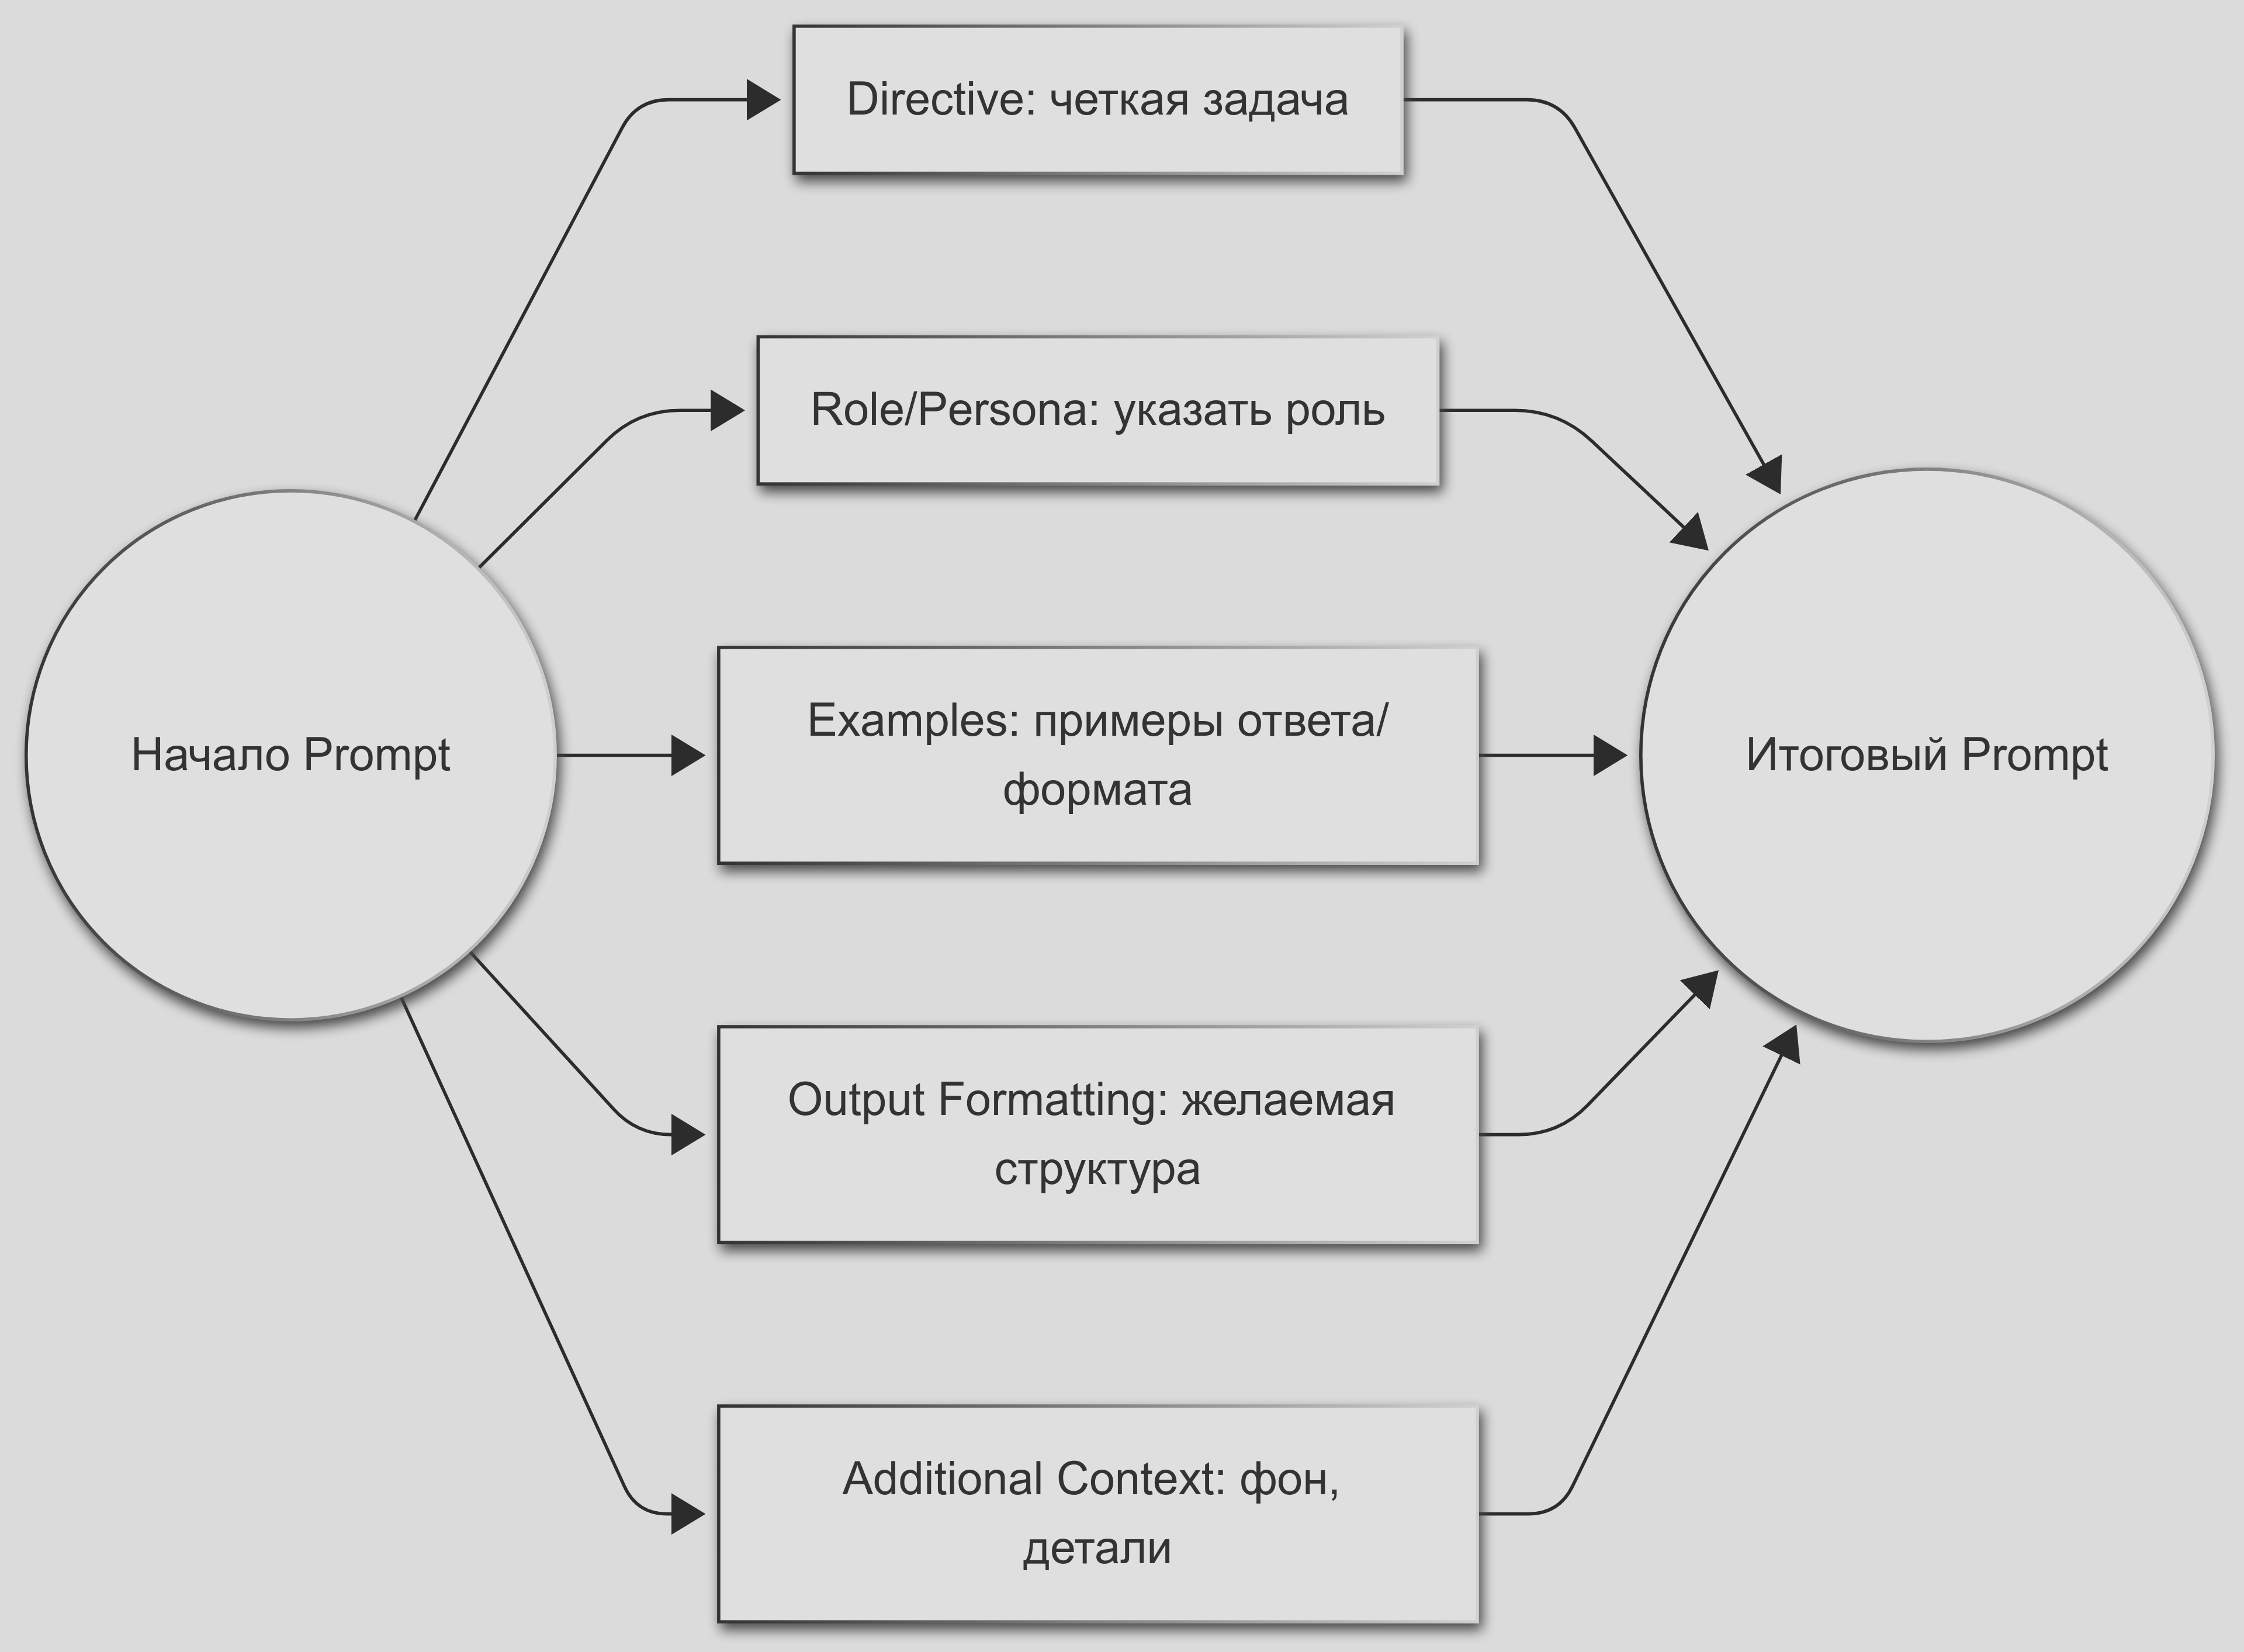
\includegraphics[width=0.8\textwidth]{picture/diploma_prompt_structure.png}
    \caption{Аспекты качественного запроса}
    \label{prompt_quality_props}
\end{figure}
Качественный запрос обычно содержит несколько ключевых элементов, обеспечивающих модели необходимый контекст\cite{learnprompt:promptstructure} они представлены на рисунке \ref{prompt_quality_props}. 
Во-первых, четкая директива (The Directive) – основная инструкция, указывающая модели, что нужно сделать.
Без ясной директивы модель может дать расплывчатый или не относящийся к делу ответ\cite{learnprompt:promptstructure}. Поэтому запрос должен содержать конкретный глагол действия и формулировать задачу напрямую (например, «составь список из пяти книг по теме...», вместо общего «расскажи что-нибудь интересное»).

Во-вторых, полезно приводить примеры (Examples) выполнения задачи, особенно для сложных или специфичных запросов. Пример(ы) в запросах демонстрируют желаемый формат или стиль ответа, помогая модели понять ожидаемый результат \cite{learnprompt:promptstructure}. Например, прежде чем попросить модель переводить предложения, можно показать один-два примера исходного текста и правильного перевода – тогда модель с большей вероятностью продолжит в заданном формате\cite{learnprompt:promptstructure}.

В-третьих, можно задать модели роль или персону (Role/Persona). Указывая, что «Ты – эксперт-историк» или «Представь себя профессиональным переводчиком», мы настраиваем тон и стиль ответа под нужный нам контекст \cite{learnprompt:promptstructure}. Такой явный контекст задаёт модели рамки: например, ответ «от лица врача» будет более формальным и содержательным в медицинской тематике. Чёткое определение роли помогает повысить релевантность и точность ответа в требуемом стиле.

Кроме того, стоит явно указывать желаемый формат вывода (Output Formatting) – например, запросить ответ в виде маркированного списка, таблицы или конкретной структуры. Наконец, полезно добавить дополнительную информацию и контекст (Additional Information): любой фон, ограничения или детали, которые могут помочь модели. Чем более конкретно очерчена задача и условия, тем более целенаправленным будет ответ модели. Интерактивные генераторы подсказок часто предлагают заполнить такие поля, как роль, цель, тон ответа, длина ответа, дополнительные детали, чтобы ничего не упустить при формулировании запроса\cite{copilotworks:promptgen}. 

Оптимизация структуры запроса. Помимо содержания, важно и то, как структурирован prompt. Рекомендуется явно разделять разные части запроса – контекст, сам вопрос, ограничения – либо визуальными разделителями, либо форматированием. Практика показывает, что использование разграничителей (делимитеров), таких как тэги XML, тройные кавычки \( \dots \) или угловые скобки для секций, повышает ясность структуры и понимание модели\cite{lakera:2025}. Например, можно оформить запрос с секциями \texttt{<context>...</context>}, \texttt{<user\_request>...</user\_request>}, \texttt{<constraints>...</constraints>}, что явно разделит вводные данные, собственно вопрос пользователя и особые требования\cite{lakera:2025}.

Хорошо структурированный ввод помогает модели не перепутать различную информацию и соблюдать заданные рамки при генерации ответа. Исследования по prompt engineering отмечают, что чёткие границы между разными типами данных в запросе значительно улучшают понимание и точность ответов модели\cite{lakera:2025}. 

Другой приём для сложных задач – это так называемый \textit{Chain-of-Thought} (цепочка мыслей). В запрос явно закладывается пошаговое рассуждение: мы просим модель сначала размышлять или вывести промежуточные шаги, прежде чем дать итоговый ответ. Такой \textit{Chain-of-Thought prompting} побуждает модель разбить сложную задачу на более простые части и решать их последовательно\cite{lakera:2025}. Исследования показывают, что без структуры модели путаются в многошаговых рассуждениях, тогда как запрос в формате «Шаг 1: \dots; Шаг 2: \dots; Вывод: \dots» даёт более логичные результаты\cite{lakera:2025}. Например, для задачи решения головоломки или математической задачи, можно явно попросить: «Реши задачу пошагово: сначала проанализируй условия, затем вычисли промежуточные значения, и в конце дай ответ». Такая структура заставляет нейросеть имитировать процесс размышления человека и выдавать более обоснованные ответы.

Уточнение и детализация. Один из принципов хорошего промпта – максимальная конкретность. Чем конкретнее и однозначнее сформулирован запрос, тем меньше шансов на размытый ответ. Практические советы включают: задавать конкретные вопросы, избегать жаргона и двусмысленностей, явно прописывать, что именно нужно на выходе\cite{lakera:2025}. Например, вместо расплывчатого «Расскажи про экономику», лучше спросить: «Дай краткий обзор современной экономики США, упомянув ВВП, уровень безработицы и основные вызовы, в \(2\)–\(3\) абзацах». Здесь чётко указана тема, аспекты, которые надо осветить, и даже желаемый объём ответа. Такой подход задаёт модели понятную задачу и формат ответа\cite{copilotworks:promptgen}.

Если требуется определённый стиль или тон, стоит это явно оговорить. Например: «Ответь дружелюбным тоном и простыми словами, понятными ребёнку \(10\) лет». Или: «Предоставь ответ формально, в академическом стиле, с цитированием источников». Эти уточнения направляют модель на нужный стиль изложения. В интерактивных генераторах подсказок подобные параметры часто выносятся как отдельные настройки \((\text{tone/style}, \text{reading level})\), чтобы пользователь не забыл их указать\cite{copilotworks:promptgen}.

Работа с длинными запросами и контекстом. Отдельная задача – как эффективно обрабатывать очень объёмные вводы или контекст. Современные LLM имеют ограничение на размер контекста (количество токенов), поэтому при превышении лимитов приходится искать обходные пути. Один из подходов – разбиение длинного ввода на части. Если у нас длинный документ, который нужно проанализировать, можно разбить его на несколько секций и отправлять модели последовательно, объединяя затем результаты. Разработчики отмечают, что в таком случае полезно между вызовами модели передавать краткие резюме предыдущих частей, чтобы сохранять контекст \cite{openai:longprompts}. Проще говоря, можно организовать итеративное суммирование: сначала модель резюмирует часть текста, затем этот резюме включается при обработке следующей части и так далее.

В ответе OpenAI сообщества отмечено: «Нужно разбить документ на секции и объединить полученные резюме. Если предыдущий контекст важен для последующих секций, попробуйте добавлять сокращённый контекст (например, заголовки или краткие выводы предыдущих секций) в новый запрос» \cite{openai:longprompts}. Такой подход позволяет обойти ограничение по токенам, жертвуя деталями, но сохраняя ключевую информацию.


Когда используется длинный контекст, есть и другой неожиданный трюк. Документация Anthropic (модель Claude) рекомендует размещать объёмные данные в начале prompt’а, а сам вопрос – ближе к концу \cite{willison:longcontext}. В тестах с моделью Claude было показано, что если длинный текст (~20k+ токенов) поместить перед инструкциями и вопросом, качество ответа заметно возрастает (в некоторых случаях на 30\% для сложных мультидокументных запросов) \cite{willison:longcontext}. Иными словами, модель лучше усваивает длинный контекст, если он дан сначала, а уже затем – конкретный запрос пользователя. Этот приём улучшает точность ответа, особенно когда нужно учесть сразу несколько больших фрагментов информации. Помимо порядка, Anthropic предлагает использовать специальные разметки, например, заключать важные цитаты из контекста в теги <quotes> и просить модель опираться именно на эти цитаты при ответе \cite{willison:longcontext}. Такой структурированный подход помогает модели сфокусировать внимание на релевантной информации даже при очень большом объёме данных. Наконец, улучшение промпта – это зачастую итеративный процесс. Рекомендуется протестировать запрос, посмотреть на ответ модели и при необходимости уточнить или переформулировать prompt. 90\% успешного prompt engineering – это эксперименты и доработки, и лишь 10\% – само изначальное написание промпта \cite{reddit:prompteng}. Можно применить рефлексию модели: например, попросить модель сначала проверить свой ответ на соответствие запросу или сгенерировать несколько вариантов ответа и выбрать наиболее консистентный. Такой приём называется self-consistency: модель генерирует несколько решений и затем путем сравнения выбирается наиболее частый или подходящий – это повышает надёжность результата при сложных вопросах. Также модель можно попросить объяснить, почему её ответ правильный, или найти ошибки – это помогает в критических задачах снизить количество фактических ошибок\cite{lakera:2025}. Эти техники относятся уже к продвинутым стратегиям (reflective prompting), где модель используется не только для выдачи ответа, но и для самопроверки или улучшения своего же вывода\cite{restack:advprompt}. Подводя итог, чтобы получить от нейросети детальный и точный ответ, нужно максимально конкретизировать запрос, структурировать его на понятные части (роль, задача, формат ответа, контекст, примеры) и при необходимости разбивать сложные задания на последовательные этапы. Внимательное отношение к формулировке prompt способно значительно повысить качество результатов модели\cite{lakera:2025}.
Ниже рассмотрим, как эти принципы реализованы в существующих инструментах и платформах для генерации и оптимизации запросов.
\subsection{Обзор существующих систем для генерации запросов} С ростом популярности LLM появилось множество инструментов, помогающих пользователям создавать или улучшать запросы. Рассмотрим несколько систем, их возможности, преимущества и ограничения:
\begin{enumerate}[label=\arabic*.]
\item Prompt Generator for ChatGPT (CopilotWorks) – веб-инструмент для быстрого составления продуманных запросов к ChatGPT и аналогичным моделям. Пользователь заполняет готовые поля: выбирает роль (эксперт, учитель, переводчик и т.д.), формулирует цель запроса, задаёт желаемый тон или формат ответа (например, совет, объяснение, краткое резюме), ограничивает объём ответа (количество абзацев или слов) и добавляет детали или контекст\cite{copilotworks:promptgen}.  На основе этих параметров генератор собирает готовый текст prompt’а, который можно скопировать и отправить в ChatGPT\cite{copilotworks:promptgen}. Инструмент фактически реализует лучшие практики создания запросов – например, предлагает указать роль модели и чётко сформулировать цель, добавлять контекст для детализации\cite{copilotworks:promptgen}. Преимущества: простота и скорость – даже неопытный пользователь за несколько кликов получит структурированный запрос. Благодаря выпадающим спискам и подсказкам снижается вероятность забыть важный параметр (тон, формат и проч.). Такой подход обеспечивает четкость и полноту промпта, что повышает качество ответа модели. Недостатки: шаблонность – система опирается на предустановленные категории ролей, тонов и т.д., что может ограничивать гибкость. Если задача нестандартна и выходит за рамки предусмотренных опций, пользователю придётся вручную дорабатывать сгенерированный prompt. Кроме того, генератор сам по себе не гарантирует идеальный результат – он лишь структурирует запрос, но не использует ИИ для его оптимизации. Тем не менее, как отправная точка для prompt engineering этот инструмент очень полезен.

\item AISEO Prompt Enhancer – автоматизированный инструмент улучшения запросов, доступный как плагин для ChatGPT. Он был разработан компанией AISEO (известной по SEO-инструментам) и позволяет автоматически перефразировать и обогащать введённый пользователем prompt. Активируется плагин ключевым словом: если начать запрос со слова “AISEO:”, подключается модуль, который перепишет последующий текст запроса более эффективным образом \cite{restack:advprompt}, \cite{whatplugin:promptenhancer}. По сути, AISEO Prompt Enhancer выступает как надстройка над ChatGPT: пользователь набрасывает черновой запрос, а плагин трансформирует его в оптимизированный, «отполированный» запрос, предназначенный для получения наилучшего ответа от модели. Преимущества: удобство – не нужно вручную вспоминать правила хорошего промпта, достаточно в свободной форме описать, что требуется, а плагин сам отформатирует и уточнит запрос. Это снижает порог входа для новых пользователей, незнакомых с тонкостями составления вопросов к ИИ\cite{whatplugin:promptenhancer}. Улучшенные запросы получаются более подробными и релевантными задаче, за счёт чего повышается качество диалога с ChatGPT. Недостатки: плагин доступен только в платной версии ChatGPT с поддержкой плагинов, что ограничивает его аудиторию. Кроме того, универсальность – плагин не обучен под конкретную доменную область, он улучшает формулировку общим образом, поэтому при очень специализированных запросах результат может быть неидеальным. Также есть ограниченная прозрачность: пользователь видит только финальный изменённый запрос, но не всегда понятно, какие правки внёс инструмент (может затруднить обучение пользователя самостоятельному составлению prompt’ов). Тем не менее, AISEO Prompt Enhancer – эффективный способ «доверить AI улучшение запросов для AI», что особенно полезно для быстрого создания запросов.
\begin{figure}[htbp]
    \centering
    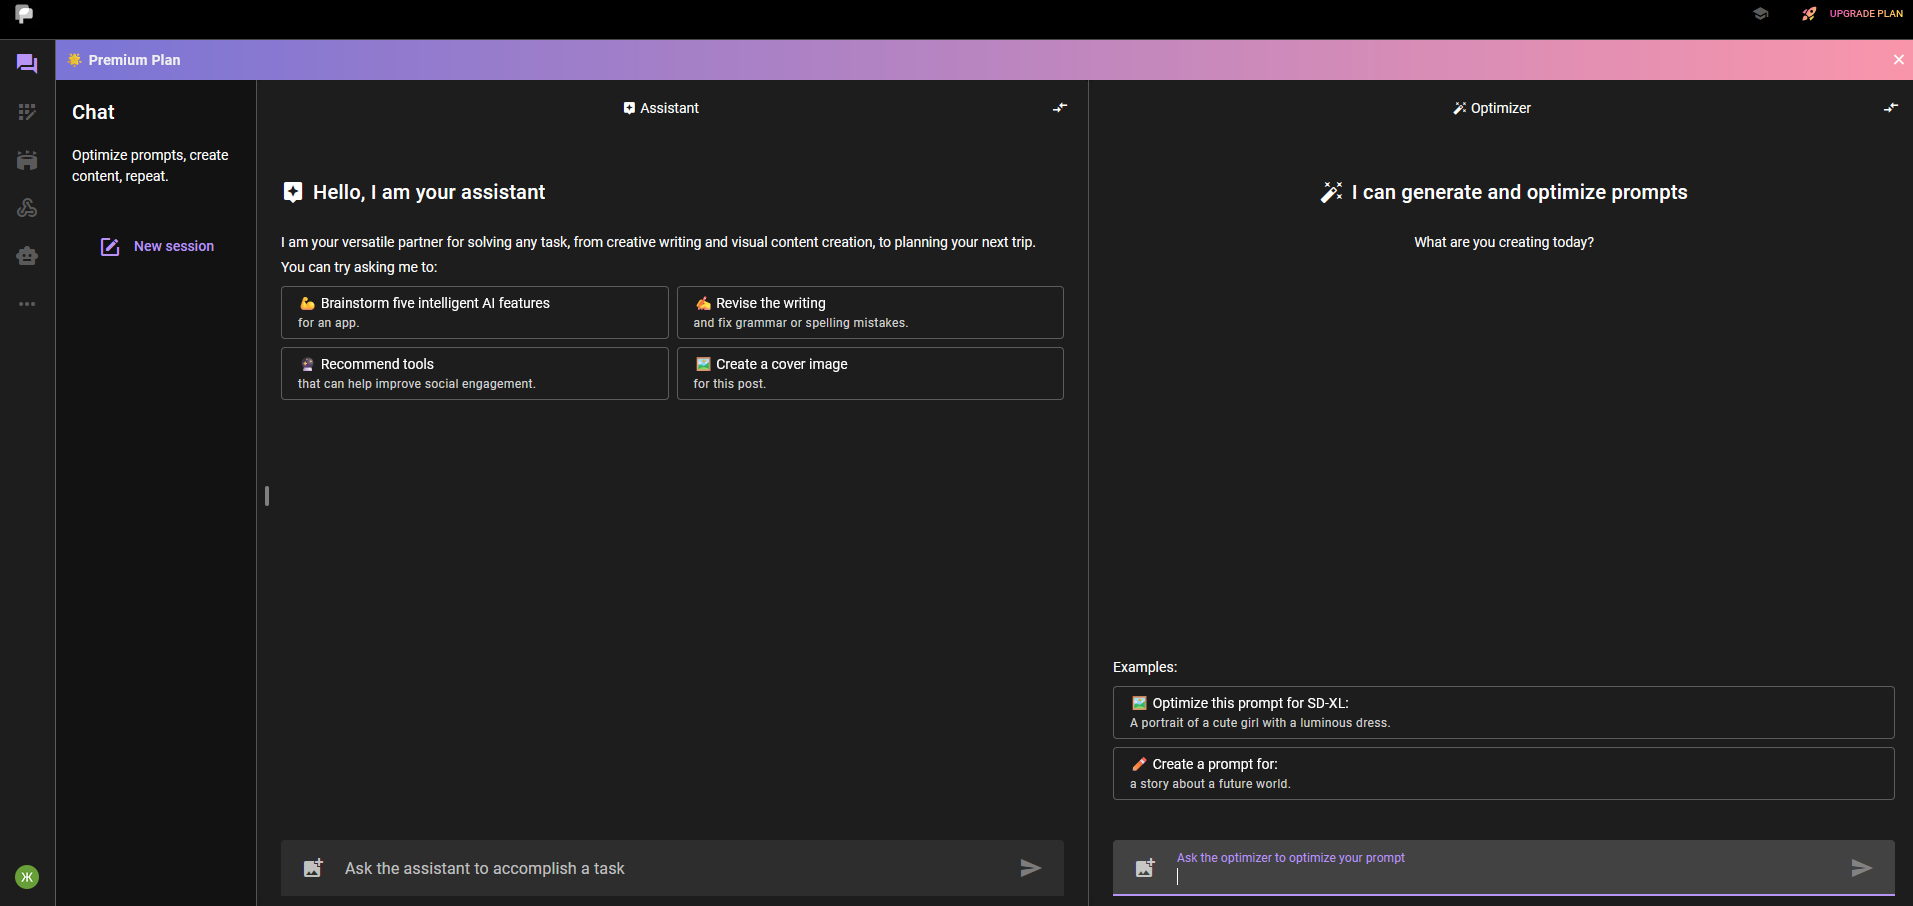
\includegraphics[width=0.8\textwidth]{picture/prompt-perfect.png}
    \caption{Веб интерфейс PromptPerfect}
    \label{prompt_perfect}
\end{figure}
\item  PromptPerfect – мощный AI-инструмент для автоматической оптимизации текстовых и визуальных запросов под различные модели. Он позиционируется как «всё-в-одном» генератор и оптимизатор промптов, поддерживающий популярные LLM (GPT-3.5/4, Claude) и генеративные модели изображений (Midjourney, DALL-E и др.) \cite{dhruvirzala:promptperfect}.Пользователь вводит исходный (сырой) запрос, выбирает целевую модель – а PromptPerfect генерирует улучшенный вариант, часто более подробный и точный. Как отмечается в обзоре, этот сервис «превращает сырые английские предложения в промпты, от которых LLM краснеют», то есть существенно обогащает и уточняет их.  Преимущества: PromptPerfect использует продвинутые техники prompt engineering под капотом. Он может автоматически добавить недостающие детали, уточнить контекст, перевести запрос на другой язык и т.п. \cite{dhruvirzala:promptperfect}. Отличительной чертой является поддержка мультиязычных промптов – инструмент способен принимать запросы на разных языках и выдавать оптимизированный prompt также на любом из поддерживаемых языков. Также сервис предлагает дополнительные функции: few-shot prompting (автоматически подставляет примеры в запрос), reverse prompt engineering для изображений (по загруженной картинке пытается сгенерировать текстовый prompt, который мог бы её описать), а также сравнение результатов разных моделей для одного и того же запроса. Наконец, у PromptPerfect есть веб-интерфейс представленный на рисунке \cite{dhruvirzala:promptperfect}. и API, что позволяет интегрировать его в рабочие процессы. Недостатки: отмечают не самую удобную UI\cite{dhruvirzala:promptperfect}. – освоить все возможности может быть непросто из-за обилия настроек (крутая кривая обучения для новичков). Кроме того, хотя базовый тариф бесплатный, для активного профессионального использования может потребоваться подписка (платный план). Ещё один нюанс – автоматическая оптимизация не всегда попадает точно в потребности пользователя, иногда может «переформулировать слишком сильно», изменив оттенки смысла. Тем не менее, выигрыш в качестве часто ощутим: инструмент действительно «добавляет детализации, повышая качество выходов ИИ»\cite{dhruvirzala:promptperfect}. В тестовом обзоре PromptPerfect получил высокие оценки за функциональность (4.7/5) и производительность (4/5), при общем рейтинге ~3.9/5 – снижают впечатление лишь нюансы интерфейса и поддержки. Это один из самых продвинутых на сегодня оптимизаторов prompt’ов, позволяющий быстро улучшать запросы для разных моделей. 
\begin{figure}[htbp]
    \centering
    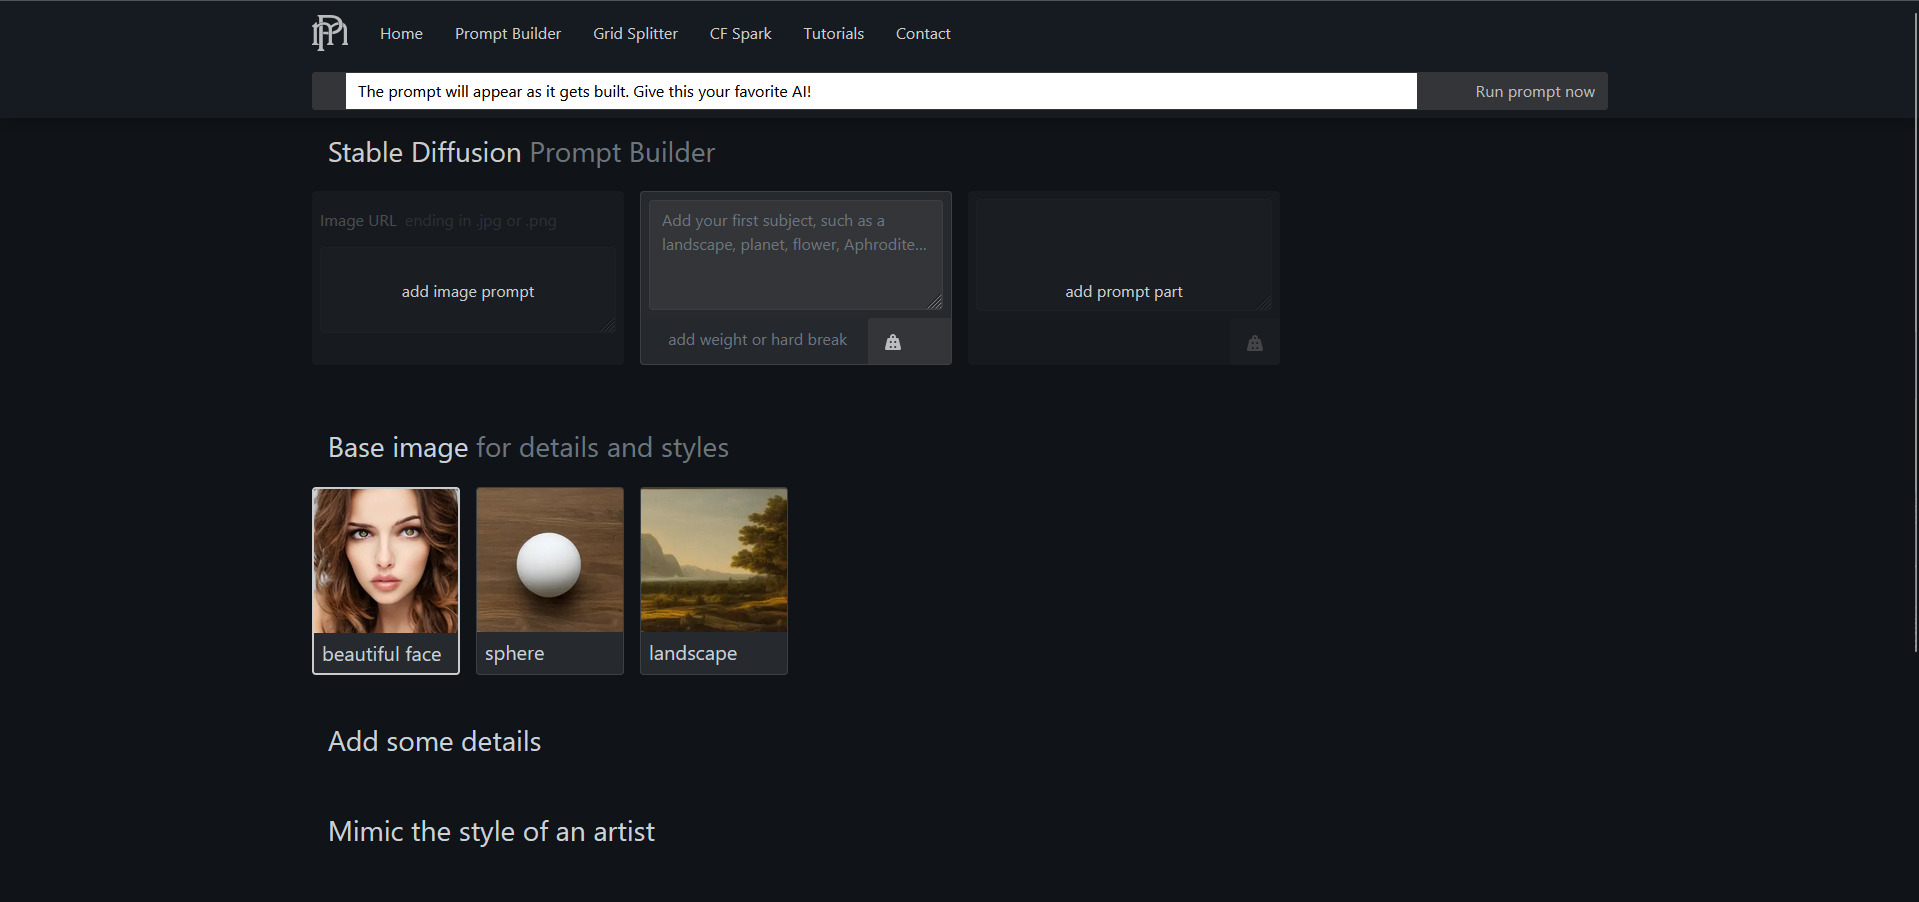
\includegraphics[width=0.8\textwidth]{picture/prompt-mania.png}
    \caption{Веб интерфейс PromptMania}
    \label{prompt_mania}
\end{figure}
\item Midjourney Prompt Generators – отдельная категория инструментов, помогающих генерировать описания для нейросетей, создающих изображения (в частности, Midjourney). Визуальные генеративные модели очень чувствительны к нюансам prompt’а: нужный стиль, детальность описания, перечисление художественных приемов. Сформулировать такой запрос сложно, поэтому появились prompt builders – интерактивные онлайн-формы, где пользователь выбирает настройки, а на выходе получает готовую строку для Midjourney\cite{promptomania:midjourney}. Пример – PromptoMANIA, бесплатный конструктор промптов для Midjourney и Stable Diffusion. . Интерфейс предлагает многочисленные опции представленные на рисунке \ref{prompt_mania}: тип сцены, художественный стиль (живопись маслом, фотореализм, акварель и т.д.), имя художника или референс (например, «в стиле Ван Гога»), параметры съемки (ракурс, объектив), качество и аспекты изображения. Преимущества: такие генераторы позволяют пользователю, не знакомому с терминологией и «секретными словами» Midjourney, легко подобрать эффектные описания. Они обычно имеют списки популярных ключевых слов: стили, жанры, освещение, цветовые схемы – которые можно комбинировать. Это гарантирует, что запрос будет содержать слова, понятные модели, и задействует известные стилистические паттерны. В результате картинки получаются более соответствующими замыслу. Кроме того, многие генераторы (PromptoMANIA, PromptHero и др.) обновляются под новые версии Midjourney\cite{promptomania:midjourney},\cite{howtoleverageai:midjourney}. учитывая лучшие практики для последней модели. Недостатки: основной минус – ограниченная креативность, поскольку пользователь выбирает из предложенных вариантов. Не все задумки может выразить готовый интерфейс, иногда требуется вручную дописать специфические детали. Также перегруженность опциями может сбивать с толку новичков – десятки выпадающих списков с художественными стилями способны запутать. Некоторые инструменты генерируют очень длинные промпты со множеством тегов – это не всегда лучше, иногда лишние теги могут внести шум. Тем не менее, для старта в работе с Midjourney они незаменимы: снижают порог входа и учат, какие слова влияют на результат. Отдельно стоит упомянуть генераторы, которые сами используют ИИ: например, сервис HowToLeverageAI предлагает сгенерировать 10 уникальных стилей одним кликом, комбинируя случайные варианты стиля для вдохновения.  Это помогает, когда хочется экспериментировать с разными художественными направлениями.

\item Stable Diffusion Prompt Generators – аналогично предыдущему, но ориентированы на модели Stable Diffusion. Поскольку SD – открытая модель, экосистема генераторов разнообразна: от простых веб-форм до открытого кода. Например, Neural Frames Stable Diffusion Prompt Generator предоставляет поле ввода для описания идеи и затем автоматически дополняет его, улучшая и уточняя для лучшего результата\cite{neuralframes:sdprompt}.  Заявлено, что он использует NLP-алгоритмы для подбора ключевых слов по введённому описанию  – то есть пользователь пишет простое описание («горный пейзаж на закате»), а система добавляет детали («HDR, 4K, dramatic lighting, by Greg Rutkowski, trending on ArtStation...» и т.п.)\cite{feedough:sdprompt}. Преимущества: экономит время и знания – не нужно самому перебирать сотни тегов, ИИ подскажет, какие ключевые слова усилят изображение. Кроме того, такие генераторы могут обучаться на больших массивах существующих промптов. В частности, открыт репозиторий модели, дообученной на 74 тысячах текстовых описаний для Stable Diffusion\cite{ollama:sdprompt}. Эта модель способна превратить краткий запрос пользователя в развернутый prompt, оптимизированный для SD\cite{ollama:sdprompt}. Такие подходы, подкрепленные данными, зачастую генерируют промпты не хуже экспертов: учитываются популярные стили, корректно расставляются весы важности слов (например, скобками или символом : в SD). Недостатки: автоматические улучшители для SD могут, подобно телефонной игре, искажать исходный замысел. Пользователь рискует получить красивый, но уже не тот кадр, что он хотел, если полностью полагается на генератор. Поэтому часто советуют использовать их как подсказку: сгенерированный prompt – основа, которую можно затем вручную отредактировать. Кроме того, некоторые инструменты (как Neural Frames) работают онлайн, и качество генерации ключевых слов может варьироваться. Однако, даже частичное дополнение запроса правильными стилевыми тегами сильно повышает качество итогового изображения\cite{feedough:sdprompt}. В целом, генераторы промптов для Stable Diffusion демократизируют использование этой сложной модели, позволяя получать красочные результаты без глубокого погружения в сообщество художников AI.

\item OctiAI Prompt Generator – относительно новая платформа (позиционируется как инструмент 2025 года), использующая комбинацию автозаполнения и ИИ для создания «идеальных промптов». OctiAI интересен своим подходом: он интерактивно задает уточняющие вопросы о вашем запросе и может автоматически заполнять ответы на них, опираясь на уже введённые данные\cite{octiai:2025}. Фактически, это полуавтоматический ассистент: пользователь описывает свой wish (желание/идею) в общем виде, далее OctiAI может сам сформулировать наводящие вопросы и сам же на них ответить, уточняя детали проекта. Сообщается, что после нескольких нажатий Enter пользователь получает персонализированный prompt, на «90\% точно отражающий его задумку», сгенерированный буквально за секунды\cite{octiai:2025}. Преимущества: OctiAI реализует принцип диалога при создании запроса – как опытный инженер по запросам, он расспрашивает о подробностях (а при авто-режиме сам логически додумывает их). Это экономит время: по сути, ИИ экстраполирует из начального замысла полный подробный сценарий. В примерах на сайте показано, как из краткой фразы «Хочу создать видео-шаблон для рекламы моего AI-приложения в TikTok» OctiAI генерирует развернутый промпт с учетом всех особенностей платформы (динамичный темп, визуальные hooks, упоминание трендов, призыв к действию и т.д.)\cite{octiai:2025}. То есть он добавляет экспертные знания о домене (TikTok-маркетинг) прямо в запрос. Для пользователя, не обладающего такими сведениями, это огромный плюс: результат – словно консультация специалиста. Недостатки: пока о нем известно не слишком много; очевидно, для такой глубокой работы OctiAI сам опирается на мощные языковые модели (возможно GPT-4), что может означать платный доступ или ограничения. Кроме того, автоматическое «додумывание» деталей за пользователя – палка о двух концах: если предположения ИИ ошибочны, итоговый prompt может увести не туда. Система заявляет 90\% точности, но 10\% расхождения могут быть критичными, особенно в творческих задачах. И, конечно, как и другие коммерческие сервисы, OctiAI – закрытая платформа, где не полностью ясно, как генерируется результат. Тем не менее, подход с автозаполнением и диалоговым уточнением представляет интересное направление: интерактивное соавторство с ИИ при создании промпта.
\end{enumerate}

Помимо перечисленных, существуют и другие решения. Например, популярное расширение AIPRM для браузера предоставляет библиотеку готовых промпт-шаблонов для ChatGPT на все случаи жизни – от маркетинга до программирования. Оно позволяет в один клик подставить сложный многошаговый запрос с переменными, экономя время. Также сообщества вроде FlowGPT обмениваются успешными промптами. Однако эти варианты меньше про автоматическую генерацию, а скорее про шаблоны и обмен опытом. В контексте же интерактивных платформ, перечисленные 5–6 систем демонстрируют разнообразные подходы: от простых форм для структурирования (Prompt Generator), через плагины и оптимизаторы на базе ИИ (AISEO, PromptPerfect), до специализированных визуальных конструкторов (для Midjourney/SD) и гибридных ассистентов (OctiAI). Каждый инструмент имеет свои сильные стороны – либо простоту, либо интеллектуальность, либо узкую заточку под конкретную модель – а пользователю и разработчику платформы важно понимать эти особенности при выборе решения.
\subsection{Архитектурные варианты платформы}
\begin{figure}[htbp]
    \centering
    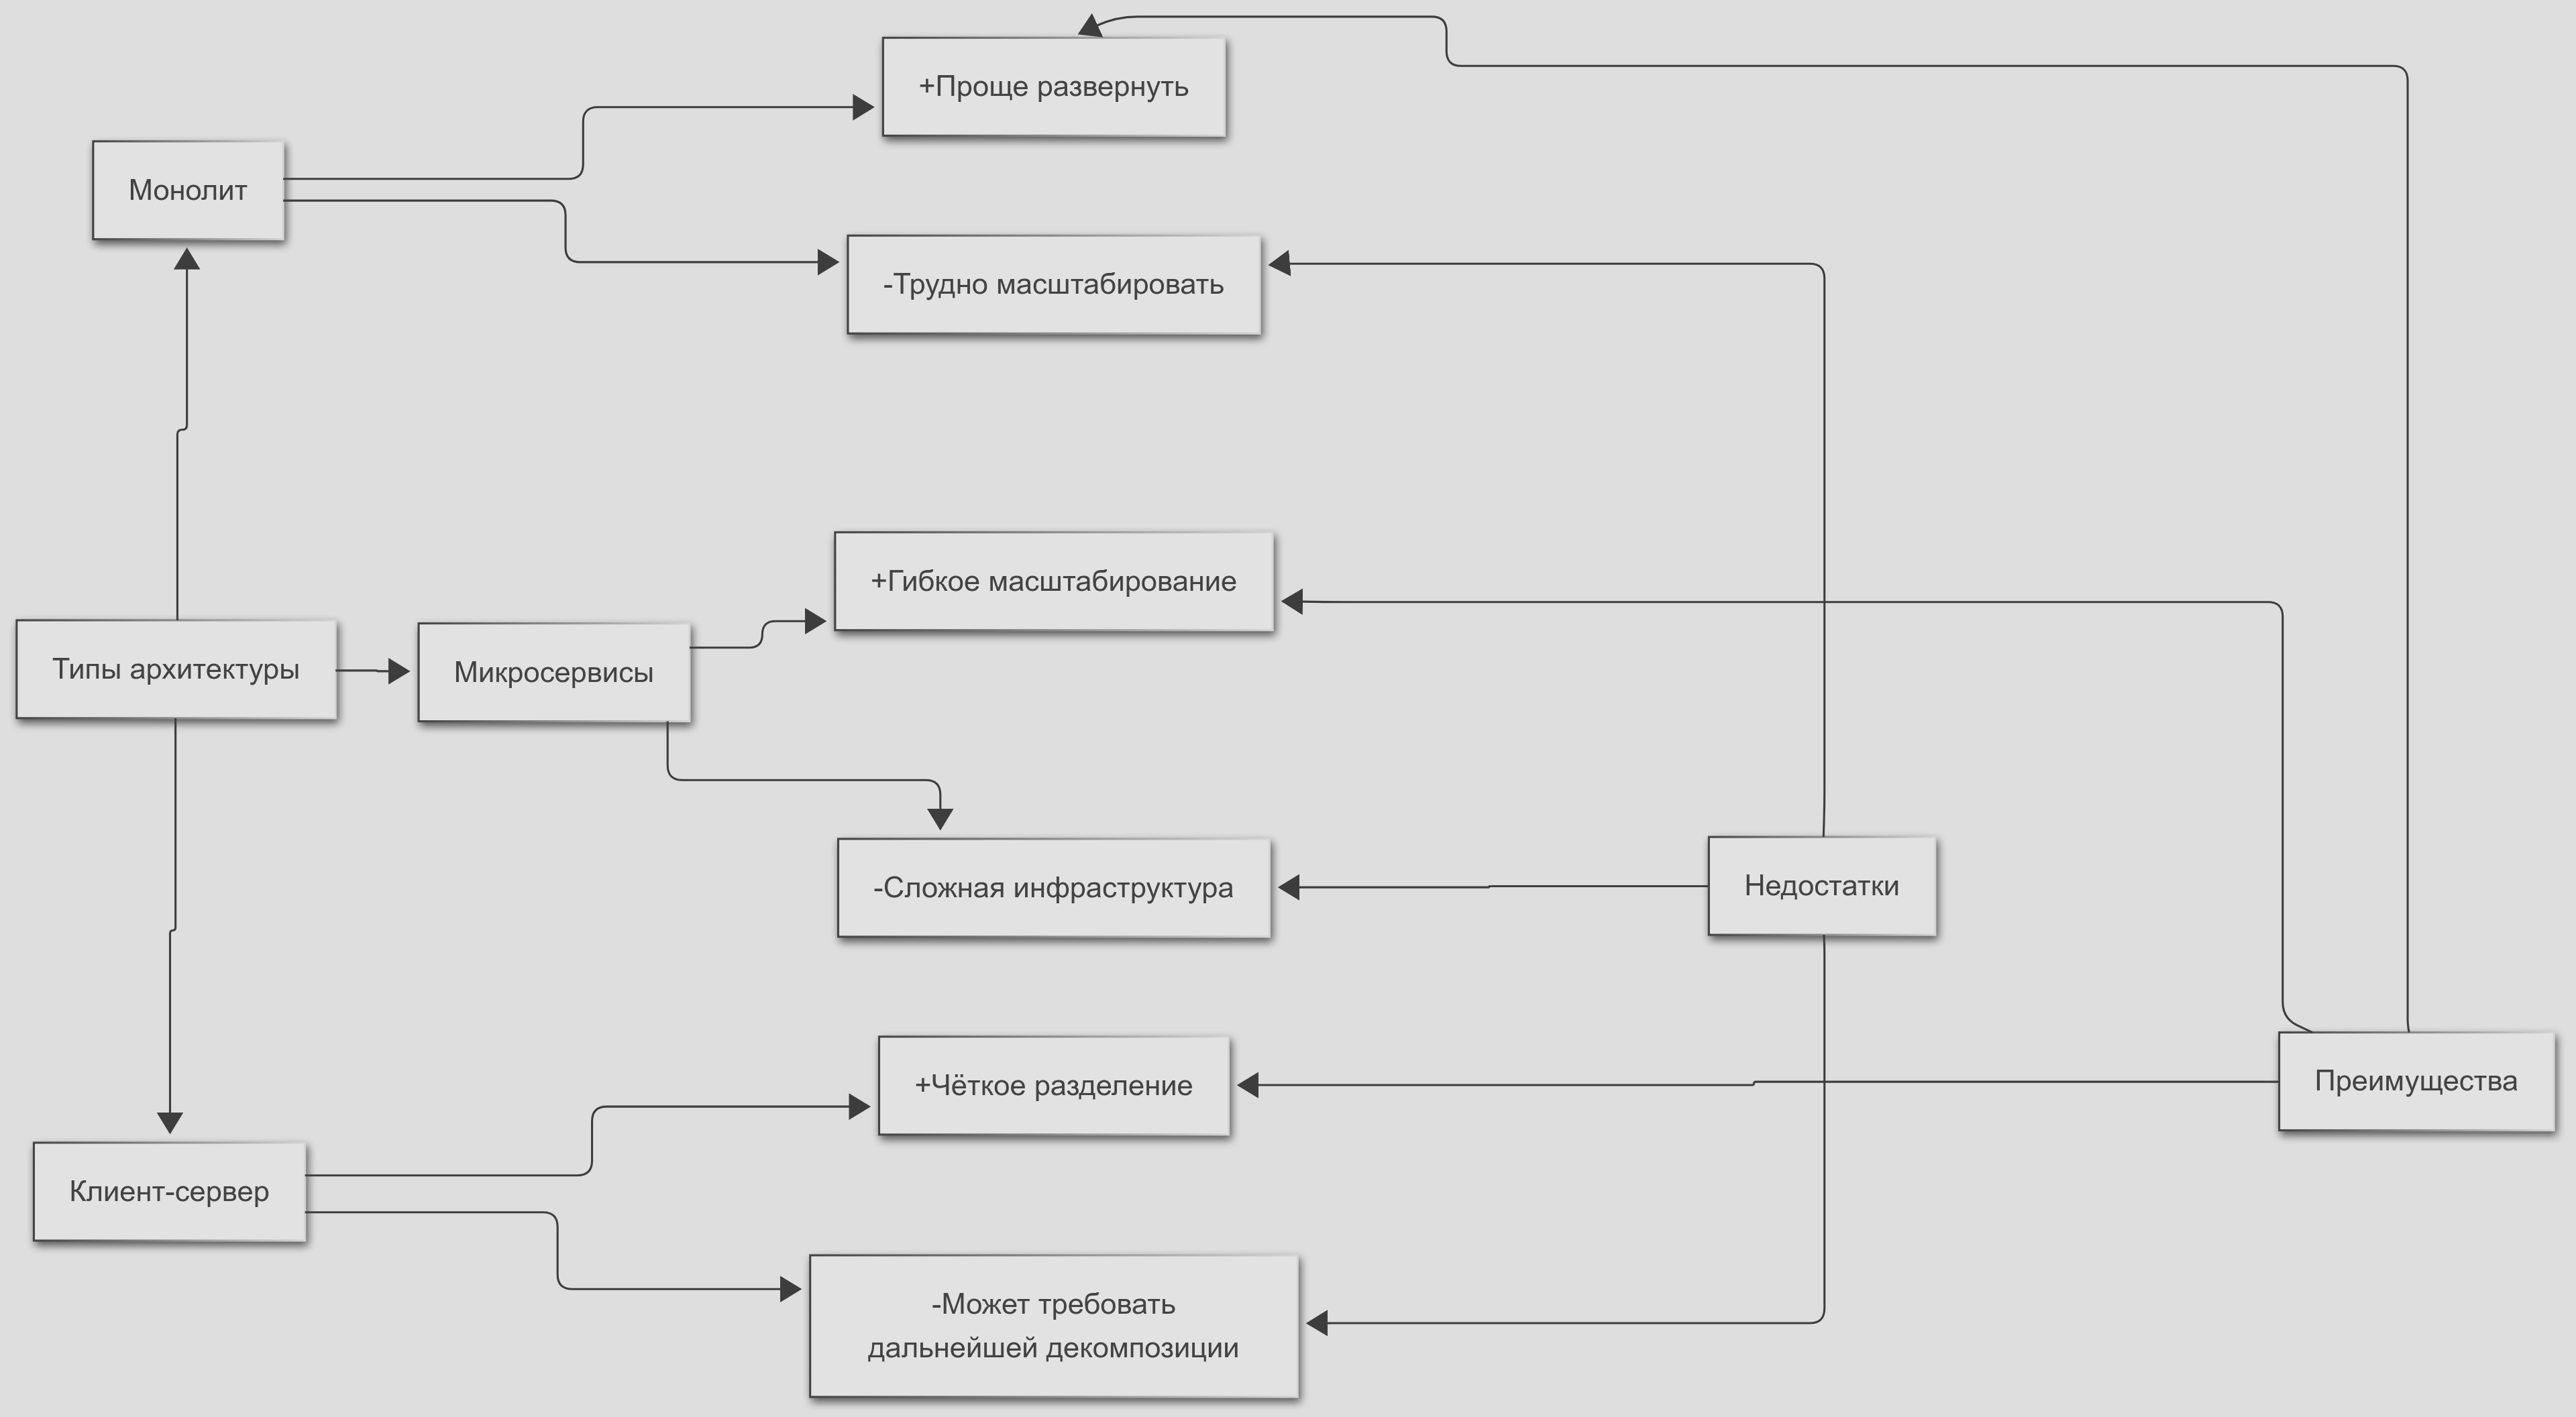
\includegraphics[width=0.9\textwidth]{picture/diploma_architecture_prototypes.png}
    \caption{Типы архитектуры с их основными преимуществами и недостатками}
    \label{architecture_prototypes}
\end{figure}
При разработке платформы для интерактивного формирования запросов важен выбор архитектуры приложения. Рассмотрим основные варианты – монолитная, микросервисная, клиент-серверная – и их плюсы/минусы применительно к нашей задаче описанные на рисунке \ref{architecture_prototypes}.

Монолитная архитектура. Монолитом называют цельное приложение, где все компоненты (интерфейс, логика, обработка данных, модель ИИ) развернуты как единое целое. Такой подход традиционно проще на начальных этапах: вся логика сосредоточена в одном кодовом базе, изменения вносятся централизованно. Преимущества: высокая скорость разработки и простота деплоя – достаточно собрать и развернуть один исполняемый файл или контейнер\cite{atlassian:microservices}. Отладка и тестирование тоже упрощены: легче отследить выполнение запроса от интерфейса до базы, когда всё в одном процессе\cite{atlassian:microservices}.  Производительность зачастую выше, так как компоненты обращаются друг к другу напрямую, без сетевых задержек – одна функция может вызывать другую в памяти. Недостатки: по мере роста проекта монолит может разрастись и стать трудным в поддержке. Малейшее изменение требует пересборки и перезагрузки всего приложения\cite{atlassian:microservices}. Масштабирование осложняется – нельзя увеличить ресурсы только для части системы, например для модуля ИИ, не масштабируя остальное. Ограничена гибкость технологий: если фронтенд, как и бэкенд,  интегрирован в монолит, они жёстко связаны, и переход на другую технологию потребует переписывания значительной части монолита. Также ошибка в одном модуле способна обрушить всё приложение (низкая отказоустойчивость)\cite{atlassian:microservices}. В современных условиях, монолитная архитектура подходит для прототипа или небольшого проекта с ограниченной нагрузкой и командой, когда важны быстрота реализации и простота. Но если платформа будет расширяться (новые модули, большое число пользователей), монолит может стать узким местом.

Микросервисная архитектура. В микросервисном подходе приложение разбивается на ряд независимых сервисов, каждый отвечает за свою функцию (например, отдельный сервис для генерации prompt с помощью ML-модели, отдельный – для управления пользователями и базой данных, отдельный – для фронтенда). Эти сервисы общаются через четко определённые API. Преимущества: гибкость и масштабируемость. Каждый микросервис можно разрабатывать, развёртывать и масштабировать независимо\cite{atlassian:microservices}. Например, если модуль улучшения запросов на основе PyTorch-модели требует много ресурсов, его можно вынести на отдельный сервер(ы) и масштабировать горизонтально при росте нагрузки, не трогая при этом остальные части системы. Обновление одного сервиса не требует останавливать всю платформу – можно выкатить новую версию микросервиса, пока другие работают. Команды разработчиков могут параллельно трудиться над разными сервисами, выбирая оптимальные технологии под задачу (один сервис на Python, другой, скажем, на Node.js, если это оправдано)\cite{atlassian:microservices}. Это ускоряет выпуск новых функций и повышает надёжность: сбой одного микросервиса не обязательно выведет из строя всю систему, остальные будут функционировать. Ключевые плюсы: агильность, независимый деплой, технологическая свобода, высокая отказоустойчивость\cite{atlassian:microservices}. Недостатки: усложняется инфраструктура. Появляется сеть сервисов – нужно настроить их взаимодействие, сервис-дискавери, балансировку, мониторинг каждого компонента\cite{atlassian:microservices}. . Отладка затрудняется: запрос пользователя может пройти через цепочку сервисов, и проследить его путь сложнее (нужна распределённая система логирования). Также микросервисы часто приводят к инфраструктурным оверхедам: каждый сервис требует контейнер, свои ресурсы, настройки CI/CD – число артефактов растёт\cite{atlassian:microservices}. Неконтролируемый рост сервисов (development sprawl) может замедлить разработку, если не вводить стандарты и не управлять зависимостями\cite{atlassian:microservices}. Для небольшой команды микросервисы могут оказаться чрезмерно сложными. Таким образом, имеет смысл переходить к микросервисной архитектуре, когда проект дорастает до масштабов, требующих отдельного масштабирования компонентов или работы больших команд параллельно. 

Клиент-серверная архитектура. Фактически, это классический подход для веб-приложений, предполагающий разделение системы на фронтенд (клиент) и бэкенд (сервер). Клиент и сервер общаются по сети (HTTP/REST или WebSocket). По сути, любое современное веб-приложение уже клиент-серверное, но важно подчеркнуть разделение ролей. Преимущества: разделение ответственности (separation of concerns) – UI и бизнес-логика отделены. Это упрощает поддержку, а также это даёт гибкость разработки: фронтенд-разработчики и бэкенд-разработчики могут работать независимо, используя специализированные инструменты для своих частей. Централизация управления на сервере упрощает обновление логики – код модели и оптимизации prompt хранится на сервере, контроль доступа, безопасность – тоже там, а клиент лишь отображает результаты. Как отмечается в литературе, клиент-сервер обеспечивает лучшую управляемость и безопасность за счёт концентрации ресурсов и данных на сервере\cite{kitrum:clientserver},\cite{enjoyalgorithms:clientserver}.


Дополнительно, можно рассмотреть и другие варианты архитектур. Например, Serverless/FaaS – когда отдельные функции (например, улучшение prompt) развёрнуты как безсерверные функции AWS Lambda или аналогов. Это обеспечивает автомасштабирование и оплату «по факту использования». Однако интеграция долгоживущих моделей в lambdas затруднительна из-за ограничений по времени выполнения и памяти. Многослойная архитектура (трёхуровневая) – где есть ещё слой базы данных, кэширующие прослойки – может применяться при большом числе пользователей и необходимости хранения истории запросов, рейтингов и т.д. Но на концептуальном уровне она схожа с клиент-сервером, просто добавляются инфраструктурные детали.

Резюмируя: для старта платформы интерактивной генерации промптов достаточно архитектуры «клиент сервер». Это разделит front/back, обеспечит удобную разработку и деплой. По мере роста нагрузки или функциональности можно выделять микросервисы – например, вынести генерацию улучшенных запросов в отдельный сервис, который можно масштабировать независимо (например, несколько инстансов с моделью на PyTorch за балансировщиком). Монолитный же вариант уместен только для простейшего прототипа или офлайн-приложения. В современном веб-окружении разделение на фронтенд и бэкенд – де-факто стандарт, обеспечивающий и модульность, и централизованное управление данными\cite{enjoyalgorithms:clientserver}. Модели и подходы для генерации улучшенных запросов

Последний аспект – как именно реализовать автоматическое улучшение промптов средствами NLP/ML в рамках выбранного технологического стека. Существуют разные подходы один из которых представлен на рисунке \ref{prompt_enchancement}: от простых правил и шаблонов до обучения нейросетей, которые переписывают запросы пользователя в оптимизированной форме. Рассмотрим несколько вариантов:

\begin{figure}[htbp]
    \centering
    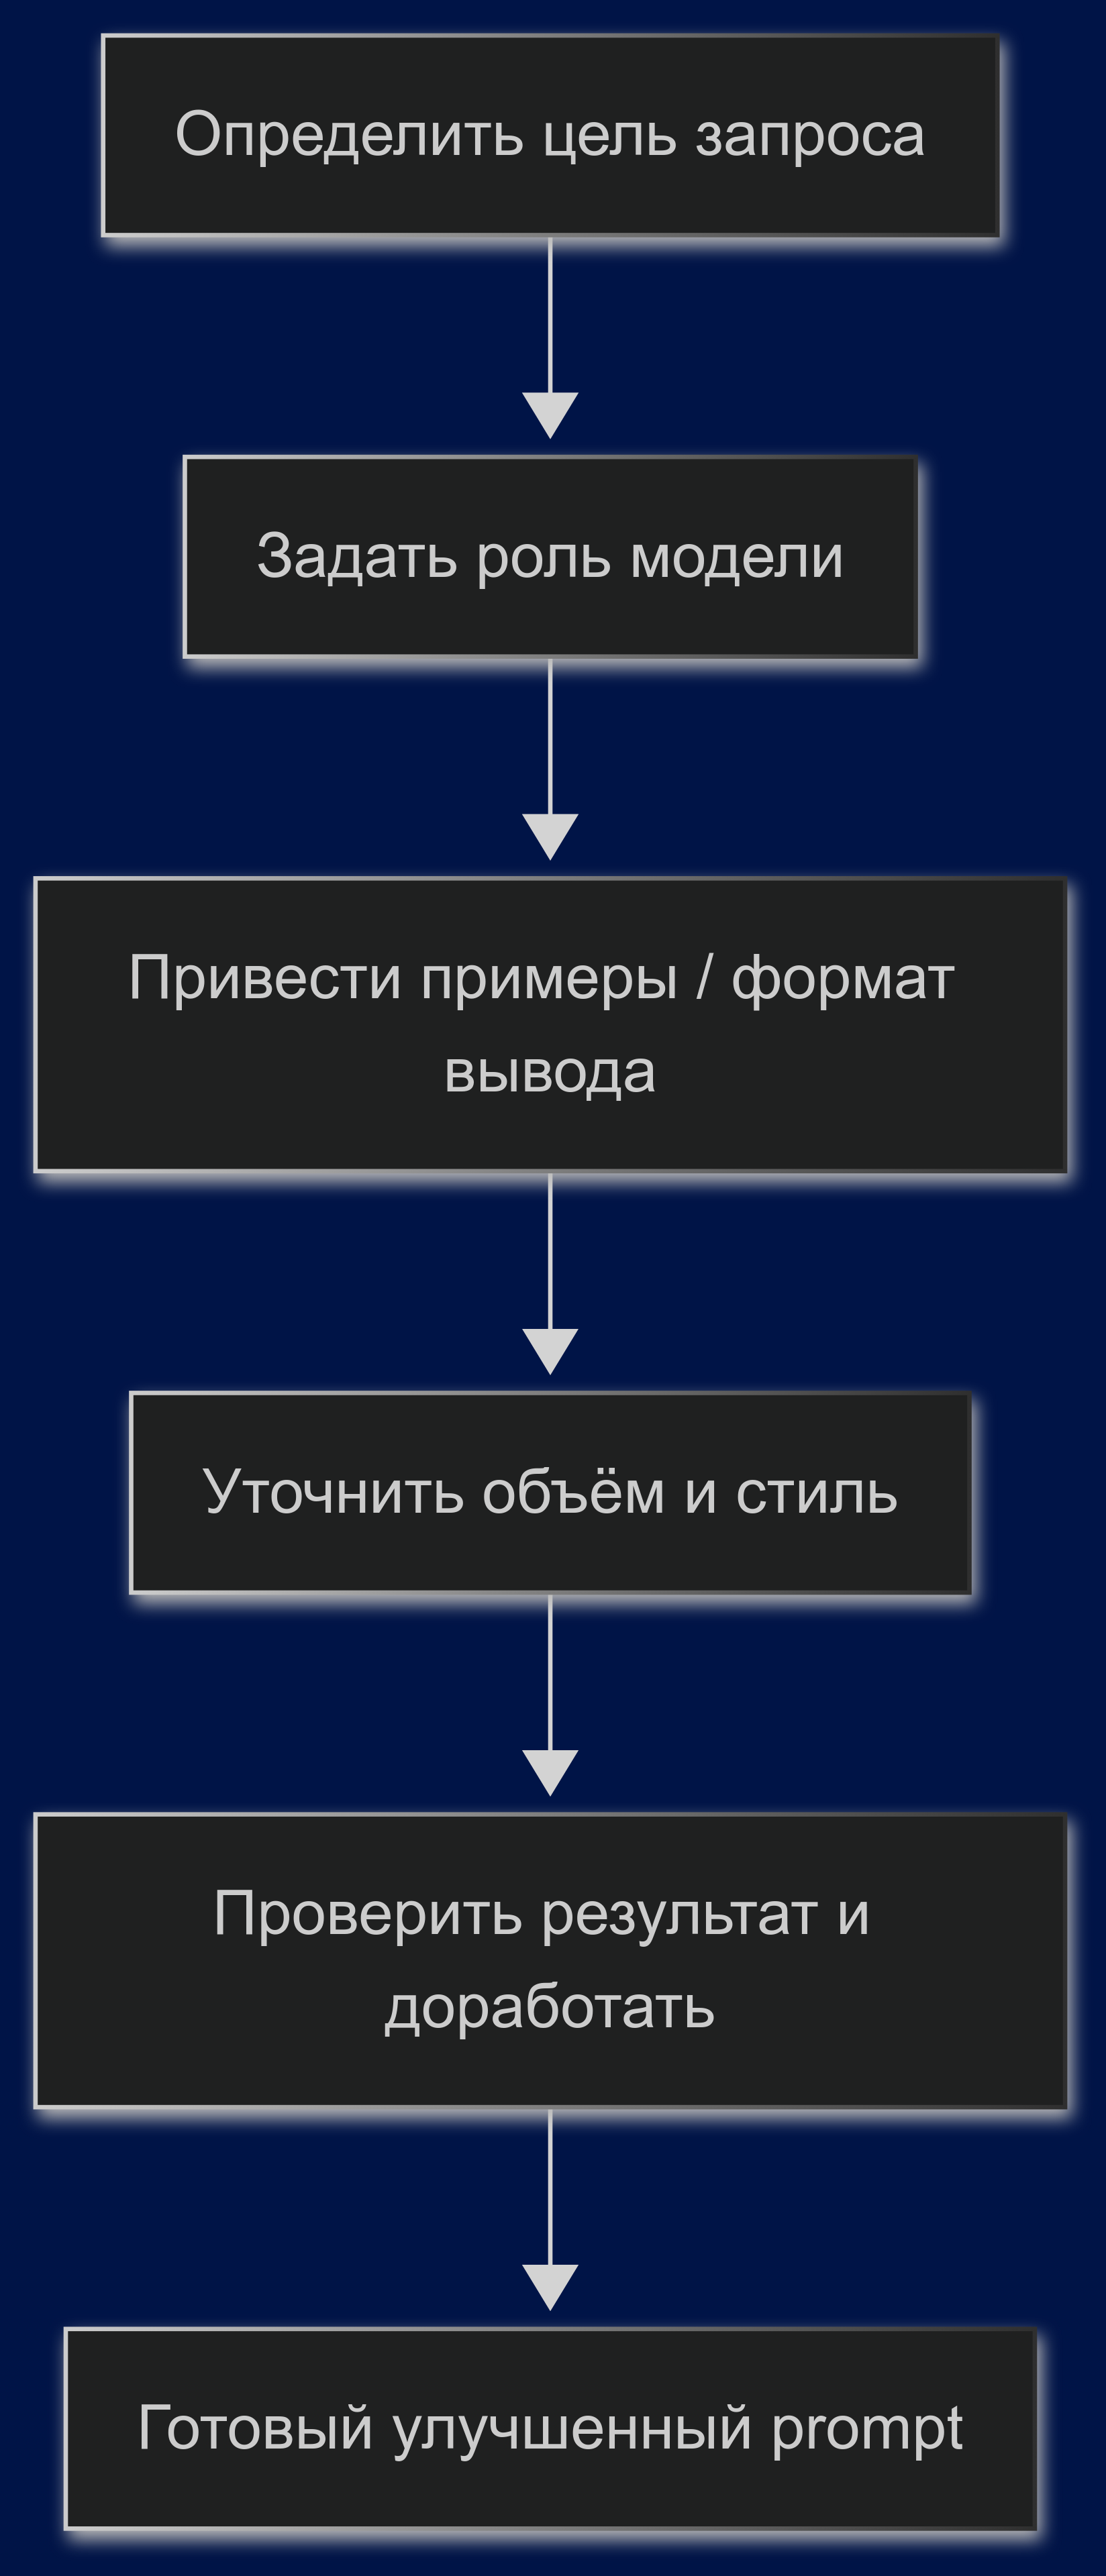
\includegraphics[height=0.7\textwidth]{picture/diploma_prompt_enchantement.png}
    \caption{Алгоритм улучшения запроса}
    \label{prompt_enchancement}
\end{figure}

\begin{enumerate}[label=\arabic*.]

\item Правила и лингвистические методы (NLP без глубокого обучения). Используя NLTK, можно выполнить базовый лингвистический анализ prompt’а: токенизация, определение частей речи, разбор предложения. Это пригодится для реализации простых эвристик улучшения. Например, можно проверить длину запроса – если он слишком короткий или состоит из одного-двух слов, платформа может подсказать пользователю добавить деталей (либо автоматически сделать запрос уточняющим вопросом). NLTK также предоставляет тезаурусы (например, WordNet) – их можно использовать, чтобы обогащать текст синонимами или более точными терминами. Предположим, пользователь ввёл: «расскажи про кошек». Автоматически можно заменить расплывчатое «расскажи» на более конкретное «дай обзор повадок домашних кошек, включая.» и т.д. – часть данных (например, список аспектов ухода за кошками) можно хранить как шаблоны (в Pandas DataFrame или БД) и подставлять по теме. Такие улучшения можно делать на основе ключевых слов: распознав слово «кошки», подставить часто запрашиваемые связанные детали (питание, здоровье, породы). Это похоже на экспертную систему: по теме запроса добавляются уточняющие фразы. Плюсы: простота реализации, полная контроль и интерпретируемость – мы точно знаем, что меняем в запросе. Минусы: сложно масштабируется на все темы – нужен словарь или база знаний, иначе ограничится несколькими предметными областями. Кроме того, без понимания контекста можно ошибиться – синоним может не подойти точно по смыслу. Однако для базовых улучшений (например, добавление в конец просьбы «дай ответ списком шагов» или «форматируй ответ в JSON», если пользователь отметил нужный формат) – правила подходят отлично. Мы можем реализовать набор опций: пользователь на фронтенде флажками выбирает «Detailed response», «Bulleted format», «Include examples» – а на бэкенде простой код на Python/NLTK добавляет соответствующие строки к prompt’у. Такая система не обучается, но повышает качество запросов по заранее заданным шаблонам.

\item Использование предобученных языковых моделей (LLM) для перефразирования. Более продвинутый путь – привлечь саму мощь LLM для улучшения prompt. Например, интегрировать вызов OpenAI GPT-4 API: передав в него что-то вроде «Преврати следующий запрос пользователя в максимально подробный и ясный prompt для ИИ: '<пользовательский запрос>'». GPT-4 способен сам сгенерировать улучшенный вариант, опираясь на свой опыт. В этом подходе мы как бы вкладываем один слой ИИ внутрь нашего приложения – мета-ИИ, который помогает обращаться к ИИ. Кстати, именно так работают плагины вроде AISEO и PromptPerfect, только используя API-ключи и, возможно, собственные модели. Плюсы: качество – современные LLM близки к уровню человека в составлении инструкций\cite{restack:advprompt}. Исследования показывают, что большие модели способны быть **«prompt engineer»-ами на уровне человека\cite{arxiv:2211.01910}. Метод, известный как Automatic Prompt Engineer (APE), поручает модели генерировать несколько вариантов инструкций и тестировать их, выбирая лучший\cite{restack:advprompt}. Это можно реализовать и онлайн: например, сгенерировать 3 версии запроса, прогнать через целевую модель (или оценить вероятности токенов) и выбрать наиболее результативный. GPT-4, конечно, ресурсозатратен, но дает отличные перефразирования. Минусы: зависимость от внешнего API (если используем его) или высокая нагрузка на сервер (если разворачивать свой LLM). Также может быть непредсказуемость – нужно тщательно настроить системные подсказки, чтобы модель-улучшатель не исказила смысл. Но в контролируемых рамках (с фиксированным prompt-шаблоном для улучшения) это работает.


\item Классические ML-алгоритмы. Можно подойти и с точки зрения обучения более простых моделей: например, классификатор, определяющий, каких элементов не хватает в prompt’е. Используя Pandas, можно проанализировать множество запросов (например, от пользователей платформы), отметить случаи, где не указана роль, или не задан формат ответа. Затем обучить модель (даже решающее дерево или логистическую регрессию) предсказывать, что нужно добавить. Однако, такие решения уступают по гибкости нейросетям. Поэтому чаще либо правила, либо уже end-to-end генерация текстов.

\item Специализированные алгоритмы оптимизации промптов. В научных публикациях появляются методы, позволяющие улучшать запросы автоматически. Помимо упомянутого APE (поиска лучшего инструктажа), есть подход Meta-Prompting – когда модель обучается сама придумывать эффективные инструкции без внешних данных.Также существуют методы с участием пользователя: интерактивные, когда система генерирует несколько вариантов перефразированного запроса, и пользователь выбирает лучший (это своего рода обучение с подкреплением от пользователя). Можно реализовать интерфейс, где после автоматического улучшения prompt показывается пользователю: «Вот так лучше? [Да/Нет]», и если нет – дать другой вариант. Получая обратную связь, система могла бы обучаться (например, методом reinforcement learning, настраивая веса модели-генератора). Это более сложная схема, но она приближает работу платформы к совместному творчеству с пользователем, а не просто «чёрному ящику».

\end{enumerate}

Важно также учесть время отклика. Улучшение запроса должно происходить быстро (идеально < 1-2 секунд), чтобы интерфейс оставался отзывчивым. Правила NLP выполняются миллисекунды, а вот вызов большой модели – может занять секунды. Поэтому, возможно, нужно кешировать результаты или использовать облегченные модели. Один из компромиссов – делать улучшение по требованию: например, если пользователь явно нажал кнопку «Enhance». Если же пользователь уже изначально дал хороший подробный запрос, система может и не тратить время (определив метрикой, что prompt достаточно длинный или содержит все элементы). Здесь Pandas пригодится для хранения статистики: например, средняя длина prompt’ов, какие улучшения чаще всего применяются – это поможет тонко настроить, когда включать ту или иную модель.

Подытоживая, возможные модели для улучшения запросов лежат на спектре от полностью ручных (статические шаблоны, правила) до полностью автоматических (нейросети, генерирующие идеальный prompt). На практике часто эффективна гибридная система: базовые вещи (формат, вежливость, явные ошибки) чинит простая логика, а тонкие стилистические или содержательные улучшения доверяются нейросети. Такой подход даст и качество, и предсказуемость.


\subsection{Вывод}
В результате проведенного анализа можно сделать следующие выводы: сочетание хорошо продуманных правил и современных моделей позволит создать платформу, где пользователь в интерактивном режиме получает подсказки и автоматическую помощь в формулировании запросов к ИИ. Применяя описанные методы детализации prompt’ов и опираясь на опыт существующих систем, можно значительно повысить качество взаимодействия с языковыми и генеративными нейросетями, делая их более доступными и эффективными инструментами. Каждый компонент стека – от Vue-интерфейса до Docker-оркестрации – играет роль в этой системе, обеспечивая удобство, масштабируемость и воспроизводимость решения. Таким образом, интегрируя технические и методологические аспекты, мы получаем мощную платформу для интерактивного prompt engineering, объединяющую лучшее из мира человеко-машинного сотрудничества.

\section{Проектирование модели платформы для интерактивного формирования
запросов к языковым и генеративным нейросетям}
\label{sec:designing}
\subsection{Целевая аудитория}
Целевой аудиторией системы являются пользователи-разработчики и художники, которые будут работать с ней на равных правах (единый уровень доступа). Платформа спроектирована с учётом их потребностей: с одной стороны, она предоставляет гибкие инструменты для тонкой ручной настройки запросов, ценимые разработчиками, с другой – наглядный и интуитивно понятный интерфейс, упрощающий работу с текстовым описанием для творческих специалистов. В следующих разделах будут подробно рассмотрены назначение системы, характеристики пользователей, требования, архитектура и используемые решения, обоснованные сформулированными техническими требованиями.

\subsection{Назначение системы}
Основное назначение разработанной системы – обеспечить пользователям возможность эффективно формировать и улучшать запросы (промпты) для различных нейросетевых моделей генерации текста и изображений.
Платформа предназначена для поддержки полного цикла работы с промптом: от начального наброска идеи до получения удовлетворительного чернового результата. Она предоставляет единое интерактивное пространство для проектирования промптов, позволяя объединить несколько функций, которые ранее требовали разрозненных инструментов.

С помощью данной системы пользователи могут создавать и редактировать текстовые описания запросов, итеративно их уточняя и детализируя. Интеллектуальные функции платформы позволяют автоматически дополнять введённый текст недостающими деталями и контекстом, что помогает менее опытным пользователям (например, художникам, не обладающим глубокими навыками работы с языковыми моделями) получить более богатые описания. Встроенный модуль оценки качества анализирует сформулированный запрос и выдает количественный показатель (в диапазоне 0–100), отражающий ориентировочное качество промпта. Это даёт возможность сразу увидеть, насколько хорошо запрос может быть воспринят нейросетью, и при необходимости внести правки до генерации результата. Кроме того, система обеспечивает преобразование формата запроса под требования конкретной целевой модели: например, адаптирует описание под синтаксис, предпочтительный для модели генерации изображений или, наоборот, для диалоговой языковой модели. Наконец, реализован режим предварительного просмотра (preview), позволяющий по нажатию кнопки отправить текущий промпт в тестовом режиме модели и получить пример отклика – сгенерированный фрагмент текста либо эскиз изображения.

Таким образом, платформа выполняет роль песочницы для промптов: разработчики могут отладить запросы для своих AI-модулей, а художники – подобрать оптимальные описания для генерации иллюстраций. За счёт возможности быстро просматривать результат и оценку, существенно сокращается число итераций «вслепую». Пользователи могут корректировать промпт до тех пор, пока не будут удовлетворены оценкой и предпросмотром, и лишь затем использовать его на основной целевой модели (например, в продакшн-системе либо в стороннем сервисе генерации). В итоге применение платформы позволяет повысить качество конечного генерируемого контента – будь то текстовые ответы модели или создаваемые изображения – и сделать процесс разработки промптов более эффективным и предсказуемым.

\subsection{ Характеристика пользователей}
\begin{figure}[htbp]
    \centering
    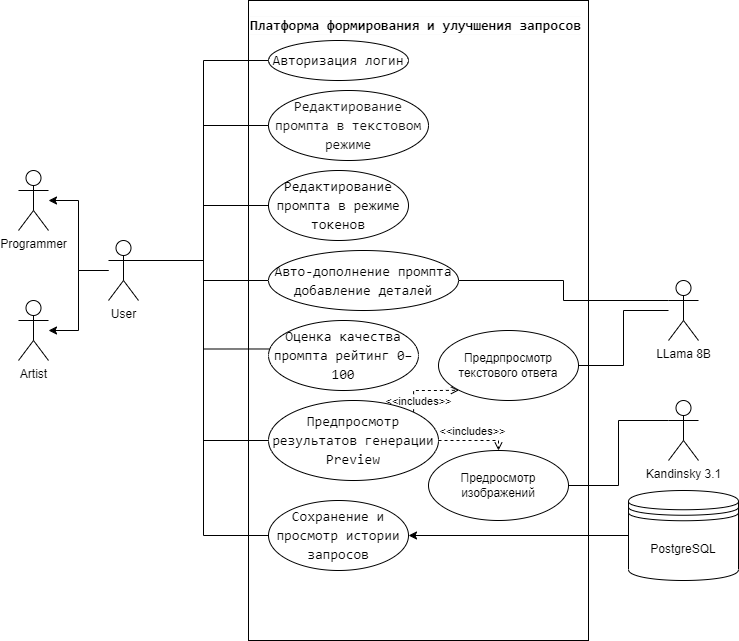
\includegraphics[width=0.8\textwidth]{picture/Диплом use case.png}
    \caption{Use case диаграмма платформы}
    \label{usecase}
\end{figure}
Как отмечалось, предполагаемые пользователи системы – это разработчики и художники, работающие с генеративными нейросетями. При проектировании платформы исходили из того, что эти две категории пользователей обладают разным опытом и целями, но обе нуждаются в удобном инструменте для создания хороших промптов. Уровень доступа в системе для них одинаковый (роль обычного пользователя), то есть все функции платформы доступны как разработчикам, так и представителям творческих профессий без каких-либо ограничений это можно заметить на диаграмме \ref{usecase}.

Разработчики (инженеры, специалисты по машинному обучению, автоААры чат-ботов и др.) используют платформу преимущественно для отладки и улучшения текстовых запросов к языковым моделям. Для них важны гибкость и точность: они оценивают промпт с точки зрения логики обработки моделью, предсказывают, приведёт ли данная формулировка к нужному ответу. Разработчики, как правило, технически подкованы, поэтому им удобен режим прямого текстового редактирования промпта, возможность вручную корректировать даже мелкие детали формулировки. Они оценят также числовой показатель качества – метрику, которая поможет количественно сравнить разные варианты запросов. В их рабочем процессе платформа вписывается как инструмент быстрого прототипирования промптов: вместо того чтобы многократно вызывать целевую модель и получать от неё ответы для сравнения, разработчик может в интерактивном режиме довести один запрос до оптимального состояния, глядя на предварительные ответы от тестовой модели и на рейтинг качества. Получив удовлетворяющий результат, он переносит этот промпт в своё основное приложение или сервис.

Художники и специалисты по визуальному контенту (например, иллюстраторы, дизайнеры, концепт-художники) используют систему в несколько ином ключе – для создания описаний, на основе которых модели типа Stable Diffusion или Kandinsky генерируют изображения. Их цель – добиться, чтобы сформулированный текст точно передавал задуманный визуальный образ и стиль. Многие художники не имеют глубоких технических знаний, поэтому для них критична простота и наглядность интерфейса. Платформа учитывает это, предоставляя интуитивно понятные средства: режим редактирования через перетаскивание токенов особенно полезен, так как позволяет им воспринимать промпт не как сплошной текст, а как набор отдельных элементов или слов, из которых складывается описание сцены. Перемещая эти элементы, художник может экспериментировать с композицией фразы, не задумываясь о синтаксисе – система автоматически обновит текст запроса. Функция автоматического дополнения детализацией полезна для художника тем, что нейросеть сама предложит дополнительные детали (например, обстановку, освещение, стилистические прилагательные), которые могут улучшить итоговое изображение. Предпросмотр через API Fusion Brain позволяет им практически мгновенно увидеть черновой результат: например, эскиз сгенерированного изображения по текущему описанию. Это визуальная обратная связь чрезвычайно ценна – художник сразу поймёт, в правильном ли направлении двигается, и при необходимости скорректирует промпт (добавит или уберёт детали, изменит формулировку).

Важно подчеркнуть, что система не вводит разграничений между разработчиками и художниками на уровне функционала. И те, и другие работают в одной среде с идентичными возможностями. Это решение принято исходя из многопрофильности современных команд: нередко разработчики и дизайнеры работают совместно над проектами с AI, и им удобно использовать единый инструмент. Платформа удовлетворяет потребности обоих типов пользователей: обеспечивает достаточно тонкий контроль для удовлетворения запросов разработчиков и одновременно остается дружественной для творческих специалистов, не требуя от них знаний программирования. Такой подход расширяет потенциальную аудиторию системы и повышает её ценность в междисциплинарных командах.

\subsection{Технические требования}

Разработка платформы базируется на предварительно сформулированных технических требованиях, отражающих необходимый функционал и ограничения системы. Требования охватывают как функциональные возможности, видимые пользователю, так и нефункциональные характеристики (производительность, совместимость, безопасность и др.). Ниже перечислены ключевые требования к системе.

Функциональные требования (основной пользовательский функционал платформы):

\begin{enumerate}[label=\arabic*]
    \item Редактирование запросов в текстовом и графическом режиме. Система должна предоставлять интерфейс для ввода и правки текста промпта вручную (классическое текстовое поле) и альтернативный интерфейс в виде списка токенов, которые пользователь может перемещать, удалять или заменять. Любое изменение последовательности токенов в графическом режиме должно незамедлительно отражаться в текстовом представлении промпта, и наоборот, обеспечивая двунаправленную синхронизацию. Должна поддерживаться работа с промптом произвольной длины (в разумных пределах, например до 1000 символов) и с различными символами, включая буквы разных алфавитов, цифры, знаки препинания и эмодзи (это важно, так как некоторые модели допускают использование эмодзи в описании изображения)\cite{fusionbrain:docs}. Пользователь должен видеть текст своего запроса и иметь возможность редактировать его удобным для себя способом.
    \item Автоматизированное дополнение (расширение) запроса деталями. Платформа должна по запросу пользователя уметь генерировать расширенную версию введённого промпта, добавляя к нему недостающую детализацию. Фактически, это интеллектуальный помощник: на основе исходного чернового текста запроса система (с помощью внутренней языковой модели) предлагает дополнительные описательные фразы, контекст или уточнения, которые могут сделать запрос более понятным для нейросети. Например, пользователь ввёл краткий запрос «кот сидит на дереве», а система может предложить дополнить: «кот сидит на дереве в лучах заходящего солнца, вокруг осенний пейзаж». Метод вызова – нажатие специальной кнопки («Дополнить»), после чего текущий текст промпта вместе с уже введёнными деталями остается, а к нему в конец или по соответствующим местам добавляется сгенерированный моделью текст (пользователь затем может отредактировать результат по своему усмотрению). Требуется, чтобы дополнение работало корректно для разных типов запросов (как описательных, так и вопросительных) и на двух основных языках (русский и английский), учитывая, что целевые модели поддерживают многоязычные запросы.
    \item Оценка качества промпта. В системе реализуется автоматическая оценка составленного пользователем запроса по шкале от 0 до 100. Эта оценка носит рекомендательный характер и должна отражать степень соответствия промпта лучшим практикам и ожидаемым требованиям модели. Пользователю отображается числовое значение или графический индикатор (например, цветовая индикация: красный – низкое качество, зелёный – высокое). Внутренне оценка может основываться на наборе правил или модели, анализирующих текст: учитывается длина запроса, специфичность формулировок, наличие деталей, отсутствие противоречий или запретов. Например, слишком короткий или расплывчатый запрос получит низкую оценку, а конкретный, содержательный запрос – более высокую. Чем более точно и понятно сформулирован промпт, тем выше должен быть рейтинг. (Это соответствует рекомендациям по промптингу: качество результатов зависит от того, сколько информации предоставлено и насколько хорошо запрос составлен)\cite{promptingguide:basics}. Данный модуль служит подсказкой: он должен быстро (в течение долей секунды) пересчитывать оценку при изменении текста и тем самым стимулировать пользователя улучшать запрос до получения приемлемого балла.
    \item Предварительный просмотр результата (preview). Одним из важнейших требований является возможность быстрой генерации чернового результата по текущему запросу. Пользователь, не покидая интерфейс редактора промптов, должен получить от системы пример отклика целевой модели – сгенерированный текст или изображение, соответствующее введённому описанию. Данный функционал реализуется двумя способами: для текстовых моделей – через APT DeepSeek, для изображений – через вызов внешнего API Fusion Brain. Платформа должна определить, какой тип результата требуется (например, по выбранному целевому движку или по контексту: если пользователь редактирует текстовый запрос для чат-бота, то генерируется текст-ответ; если промпт адресован модели изображения, то генерируется картинка). После нажатия кнопки «Preview» происходит обращение к соответствующей модели:
    \begin{enumerate}[label=4.\arabic*]
        \item В случае текста: DeepSeek генерирует продолжение или ответ на заданный промпт (необходимо ограничить размер выдаваемого фрагмента, например 1000 символов, чтобы получить быстрый предварительный ответ). Полученный ответ отображается на экране (например, в отдельном поле под запросом).
        \item В случае изображения: сервер отправляет запрос к API Fusion Brain (модель Kandinsky 3.1) с параметрами генерации (тип = GENERATE, текст запроса и др.). В ответ через некоторое время возвращается сгенерированное изображение, которое выводится пользователю (в виде эскиза, уменьшенного изображения либо полноразмерного, если позволяет интерфейс). Пользователь должен иметь возможность быстро увидеть этот результат в интерфейсе, без ручного перехода на внешние сервисы. Например, платформа может отобразить сгенерированную картинку прямо в браузере. В обоих случаях предварительно сгенерированный контент носит ознакомительный характер – он позволяет оценить, что примерно получится из данного промпта. Пользователь, проанализировав результат, может тут же подправить запрос и снова вызвать preview, добиваясь улучшения. Важно, чтобы среднее время получения предпросмотра было приемлемым: для текста это обычно менее 5 секунд, для изображения – порядка 5–15 секунд (зависит от мощности сервера и скорости внешнего API).
    \end{enumerate}
\end{enumerate}
Помимо основных функций, вытекают и общие технические требования к системе: 
\begin{enumerate}[label=\arabic*]
    \item Интуитивность и удобство интерфейса. Пользователи разных категорий должны легко освоить работу с платформой. Интерфейс должен быть локализован (минимум на русском языке, так как аудитория – в том числе русскоговорящие художники). Все элементы (кнопки «Оценить», «Предпросмотр», переключатель режима редактирования и т.д.) должны быть наглядно обозначены. Требуется реализация динамического обновления – например, пересчёт оценки качества без перезагрузки страницы, мгновенная синхронизация текстового и токенного представления запроса. Это подразумевает использование возможностей SPA (Vue.js) для реактивности.
    \item  Производительность и масштабируемость. Платформа должна эффективно работать при одновременном использовании несколькими пользователями. Ожидается, что число активных пользователей невелико (например, сотни или тысячи, поскольку целевая аудитория – команда разработчиков или художников или отдельные специалисты), однако архитектура не должна иметь жёстких ограничений на масштабирование. Серверная часть на FastAPI должна обрабатывать параллельно несколько запросов (благодаря асинхронности и производительности FastAPI это достижимо)\cite{fastapi:practicum}. Важно оптимизировать время отклика: интерактивные операции (редактирование, оценка) происходят почти мгновенно, а более тяжёлые (предпросмотр) – максимально быстро для выбранных моделей.  Для Fusion Brain API и DeepSeek API можно предусмотреть обработку в асинхронном режиме (не блокируя основной поток приложения во время ожидания ответа от внешнего сервиса).
    \item Ограничения и обработка ошибок. Система должна корректно обрабатывать нестандартные ситуации: слишком длинные запросы (превышающие лимиты модели) – выдавая предупреждение или автоматически укорачивая до допустимого размера; недопустимые символы – экранируя или удаляя их; отсутствие связи с внешним API – уведомляя пользователя о невозможности получить preview в данный момент. Все входные данные валидируются (FastAPI и Pydantic обеспечивают автоматическую проверку типов и форматов на уровне API\cite{yandex:fastapi}), а при обнаружении некорректных – сервер возвращает понятные сообщения об ошибках. Важным требованием является устойчивость: сбой одной из компонентов (например, недоступность БД или падение модели) не должен приводить к неуправляемому краху всего приложения – должны быть предусмотрены механизмы возврата в консистентное состояние или перезапуска сервиса.
    \item Совместимость и развиваемость. Платформа должна быть построена с использованием стандартных веб-технологий, обеспечивающих её совместимость с основными браузерами (Chrome, Firefox, Safari, Edge) без необходимости установки специальных плагинов. Желательно соблюдение принципов адаптивности интерфейса (возможность работать на экране ноутбука, настольного ПК, и, по возможности, на планшете). В архитектуре и коде должны быть заложены возможности расширения: например, добавление новых моделей (если в будущем понадобится поддержать другую нейросеть для генерации аудио или видео, или добавить ещё одну языковую модель) не должно требовать переписывания системы с нуля. Это означает, что компоненты (модуль оценки, модуль реструктуризации) должны быть реализованы конфигурируемо, с возможностью подключения новых правил или алгоритмов.
\end{enumerate}
Сформулированные выше требования служат основой для проектирования системы. На их основании в следующих разделах выбираются соответствующие методики и технические решения, обосновывается архитектура, алгоритмы работы и необходимые ресурсы. Соблюдение этих требований должно обеспечить, что итоговая платформа будет полнофункциональной, удобной для целевых пользователей и надёжной в эксплуатации.
\subsection{Алгоритмическое и программное обеспечение}
В данном разделе описаны ключевые алгоритмы, реализующие функции платформы, а также используемое программное обеспечение (библиотеки, фреймворки) и принятые при разработке технические решения. Проектирование алгоритмов велось на основе требований, сформулированных в разделе 3.4, – каждый функциональный пункт соответствует определённой методике реализации. Также рассматриваются программные средства, обеспечивающие выполнение этих алгоритмов.

\begin{figure}[htbp]
    \centering
    
\includegraphics[width=1\textwidth, height=100]{picture/diploma-inter-algo-1.png}
    \caption{Алгоритм редактирования запроса}
    \label{algo-1}
\end{figure}

Редактирование запросов (текст и токены). Алгоритм редактирования в текстовом режиме тривиален и отображён на диаграмме \ref{algo-1}: пользователь вводит или изменяет строку символов, которая хранится во внутреннем состоянии приложения. Более интересен алгоритм представления промпта в виде набора токенов. Здесь под токеном понимается либо отдельное слово, либо устойчивое словосочетание – на практике для упрощения можно принять токенизацию по пробелам и знакам пунктуации (каждое слово или знак рассматривается как отдельный элемент). При переключении в режим токенов исходный текст промпта разбивается на массив токенов. Этот массив отображается на экране, например, в виде последовательности интерактивных «карточек» с текстом. Для реализации перетаскивания (drag-and-drop) используются возможности HTML5 DnD или готовые компоненты из экосистемы Vue (например, Vue.Draggable). Далее массив конкатенируется обратно в строку с добавлением пробелов – таким образом получается обновлённый текст промпта. Vue.js автоматически отследит изменение массива токенов и обновит связанную переменную текста (или наоборот, если связность сделана через одно хранилище состояния). Таким образом обеспечивается одновременная актуализация обоих представлений. Кроме того, если пользователь в текстовом поле ручным образом изменяет текст (например, дописывает новое слово), алгоритм распознаёт это (через реактивный watcher) и пересобирает список токенов заново. В результате редактирование может происходить параллельно в любом формате без рассинхронизации. Этот алгоритм достаточно прост (основные операции – разбиение строки и объединение списка), поэтому не нагружает систему даже при длинных промптах.
\begin{figure}[htbp]
    \centering
    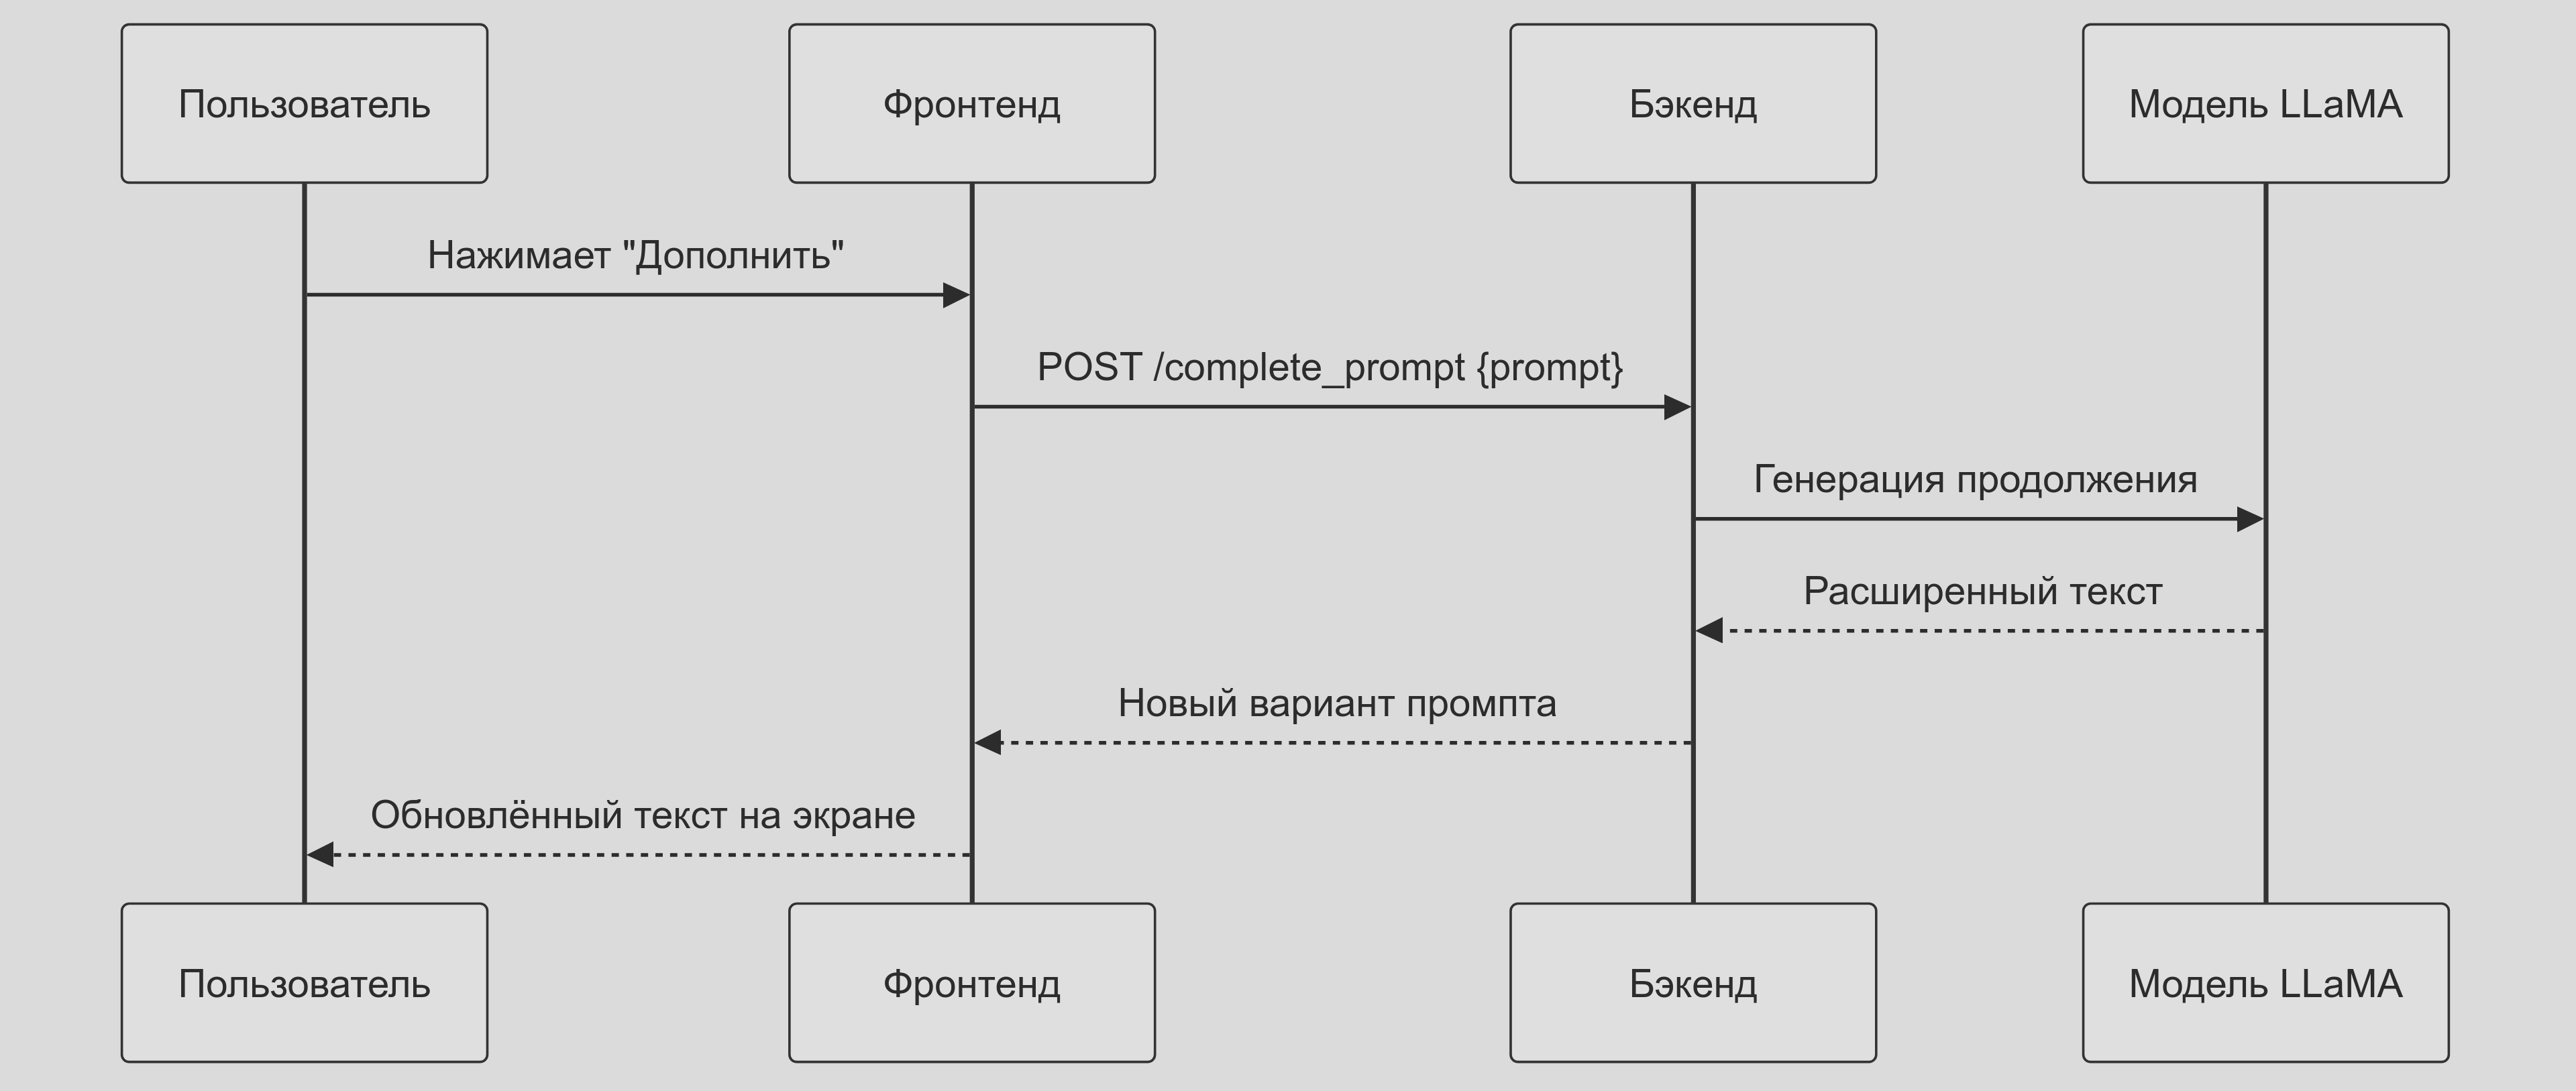
\includegraphics[width=1\textwidth]{picture/diploma-inter-algo-2.png}
    \caption{Алгоритм дополнения запроса}
    \label{algo-2}
\end{figure}
Дополнение запроса детализацией. Данная функция опирается на алгоритмы генерации текста с помощью модели DeepSeek. При нажатии пользователем кнопки «Дополнить» клиент отправляет текущий текст промпта на сервер (эндпойнт /complete prompt). Сервер вызывает специальную функцию, которая обращается к API модели DeepSeek. Алгоритм представлен на диаграмме \ref{algo-2} и может быть описан следуюoей последовательностью:
\begin{itemize}
    \item клиент отправляет исходный текст на сервер;
    \item сервер формирует входную подсказку (Prompt) для DeepSeek, используя шаблон <<Расширь описание \dots>;
    \item модель генерирует продолжение с учётом заданных параметров (длина, температура и пр.);
    \item полученные фразы автоматически добавляются к исходному промпту.

\end{itemize}

Алгоритмически, основная интеллектуальная работа здесь выполняется языковой моделью. Предусмотрены некоторые меры для улучшения результата: например, если модель начала повторять исходный текст или уводит в сторону, сервер может отсечь первые токены генерации до появления новых данных. Поскольку DeepSeek предоставляется готовым REST API, она интегрирована через Rest API.  Таким образом, алгоритм дополнения промпта сводится к задаче последовательного генерирования текста нейросетью – типичная задача, для которой используются наработки и функции библиотек машинного обучения.

Оценка качества промпта. Алгоритм оценки – это комбинация эвристических правил и, потенциально, моделей машинного обучения. В рамках данного проекта реализуется более простой, объяснимый подход на основе метрик текста. При вызове функции оценки (пользователь нажимает, либо автоматически при изменениях) клиент отправляет промпт на сервер (/evaluate prompt). Сервер вызывает функцию evaluate prompt(text), которая выполняет следующие шаги:
\begin{enumerate}[label=\arabic*]
    \item Анализ длины и полноты. Вычисляется длина текста (в словах или символах). Если длина меньше некоторого порога (например, менее 3–5 слов), выставляется низкий базовый балл (такие запросы, как правило, слишком общие). Оптимальный диапазон длины – эмпирически, скажем, 10–20 слов для текстовых моделей, 5–15 слов для графических (со стилевыми тегами). Если запрос очень длинный (более 50–100 слов), тоже может снижаться балл – за избыточность.
    \item Проверка специфичности. Алгоритм может содержать список «пустых» слов (типа «изобрази», «сделай» – паразитные для промпта генерации изображения) и, наоборот, проверить наличие содержательных прилагательных, уточняющих фраз. Например, наличие хотя бы одного прилагательного или определяющего оборота может добавлять балл, так как уточняет запрос. В руководствах по промптингу подчёркивается, что специфичность и контекст повышают качество результата\cite{promptingguide:basics}. Следовательно, если промпт содержит детали (например, указание стиля, времени суток, эмоций персонажа и т.п.), это положительно влияет на оценку.
    \item Ясность формулировки. Проверяется, нет ли в тексте двусмысленностей или нерелевантных фрагментов. Этот пункт сложнее формализовать, но можно частично оценить по структуре предложения: если промпт состоит из нескольких несвязанных предложений или вопросительных форм (которые могут сбить модель), балл снижается. Например, запрос вида: «Нарисуй кота. Может дерево? Нет, лучше солнце.» явно плох по структуре – алгоритм может обнаружить наличие нескольких предложений или вопросительных знаков и снизить оценку.
    \item Учет модели. Если уже выбрана целевая модель, алгоритм может использовать разные профили оценки. Например, для изображения ценятся указания на визуальный стиль (реалистичный, мультяшный, 3D-рендер и т.д.) – их наличие повышает балл. Для текста ценится чётко поставленный вопрос или задача – наличие вопросительного знака при обращении к чат-боту, наоборот, может быть положительным (для диалоговой модели).
    \item Формирование итогового балла. Балл вычисляется на основании нескольких компонент. Например: score = length score + specificity score + clarity score + model adaptation score. Каждая в диапазоне 0–25, суммируя до 100. Данный подход позволяет объяснить оценку: «Ваш промпт слишком короткий, добавьте деталей» – если низкий length score, «промпт содержит противоречивые указания» – если clarity score низкий, и т.п.
    \item Возврат балла. Сервер возвращает число от 0 до 100. Клиент отображает его, при этом возможно сопроводить коротким вердиктом (например, «Среднее качество» при 50–70, «Отличный промпт» при >80).
\end{enumerate}
Этот алгоритм легко модифицировать под новые критерии, его можно обучить (если бы были данные промптов с оценками, можно настроить веса правил или модель классификатор). Пока же он реализован на основе здравого смысла и рекомендаций по написанию промптов\cite{vc:prompt}, \cite{promptingguide:basics}. Программно реализация выполнена на Python: для лингвистического анализа можно использовать стандартные библиотеки (например, NLTK или simple pos-tagging для выделения частей речи, если нужно искать прилагательные). Однако в простейшем варианте достаточно операций над строками, что не требует внешних зависимостей. Важно отметить, что время выполнения этого алгоритма невелико – порядка нескольких миллисекунд, т.к. текст анализируется без тяжёлых моделей. Поэтому оценка может обновляться практически мгновенно при каждом изменении запроса.

Реструктуризация промпта под модель. Алгоритм реструктуризации заключается в применении определённого набора правил трансформации текста в зависимости от целевой модели. Эти правила основаны на известных требованиях/особенностях промптов для разных генераторов. Реализация может быть как шаблонной (набор if/else в коде), так и с участием нейросети. В первом прототипе достаточно правила:
\begin{enumerate}[label=\arabic*]
    \item Для модели изображения (Fusion Brain/Kandinsky):\begin{enumerate}[label=1.\arabic*]
        \item Удалить обращение к модели в повелительном наклонении. Например, фразы вроде «нарисуй», «сгенерируй картинку:» не несут содержания для модели, их следует убрать.
        \item Выделить негативные указания. Если в тексте есть конструкции «не используй ...», «без ...», они преобразуются в отдельный негативный промпт (для Kandinsky предусмотрено поле negativePromptUnclip). Алгоритм: найти ключевые слова «не», «без», собрать последующие слова до запятой или конца – это будет отрицательный промпт.
        \item Проверить язык описания. Kandinsky 3.1 понимает и русский, и английский\cite{fusionbrain:docs}. Здесь не нужно перевода, но важно убедиться, что промпт цельный на одном языке (смешение языков нежелательно).
        \item Возможно, добавить стандартные атрибуты, если их нет: например, многие художники добавляют стилистические теги («арт», «реалистично», «аниме-стиль»). Если пользователь ничего про стиль не указал, алгоритм мог бы по умолчанию добавить что-то нейтральное (но чаще стиль лучше оставить пустым – Fusion Brain и так принимает параметр style, который по умолчанию = NONE).
        \item Итогом алгоритма станет либо изменённая строка промпта (если мы решим не разделять, а просто убрать лишние слова), либо структура с полями: main\_prompt и negative\_prompt. Сервер знает, что для FusionBrain надо использовать оба. На стороне клиента это может отобразиться или остаться скрытым – по решению.
    \end{enumerate}
    \item Для языковой модели (DeepSeek или подобные): 
    \begin{enumerate}[label=2.\arabic*]
        \item Если исходный промпт больше походил на описание картинки (например, перечисление объектов без вопроса), а цель – текст, возможно, стоит преобразовать его в форму задания или вопроса. Например, промпт «кот сидит на дереве ночью» для чат-бота LLM непонятен – алгоритм мог бы добавить «Опиши сцену: кот сидит на дереве ночью.» либо обернуть это в вопрос: «Что произошло: кот сидит на дереве ночью? Расскажи историю.» Но такие преобразования могут оказаться слишком творческими. Вероятно, лучше минимально менять текст.
        \item Удалить специфические теги или слова, характерные для графических запросов (типа «4K», «highly detailed») – в текстовой модели они бессмысленны.
        \item Если целевая языковая модель – диалоговая, можно добавить, например, пометку «User: \{prompt\} Assistant:» для внутренних нужд (в LLaMA 2 есть формат входа с метками ролей).
    \end{enumerate}
\end{enumerate}
В целом алгоритм реструктуризации во многом состоит из поиска и замены. Он оперирует строкой: ищет определённые шаблоны (регулярные выражения или ключевые фразы) и преобразует их. Его сложность невысока, реализация на Python с библиотекой re или просто методами строк. При расширении на новые модели (например, аудиогенерация) нужно будет добавить соответствующие правила (например, убрать слова «изображение», заменить их на «звук», и т.д.).

Предварительный просмотр результата представлен, как последовательность показанную на диаграмме \ref{algo-3}
\begin{figure}[htbp]
    \centering
    
\includegraphics[width=1\textwidth]{picture/diploma-inter-algo-3.png}
    \caption{Алгори предпросмотра  результата запроса}
    \label{algo-3}
\end{figure}


Данная последовательность заключается в седующих шагах:
\begin{itemize}
    \item пользователь нажимает кнопку «Предпросмотр»;
    \item клиент отправляет запрос \texttt{/preview} с текстом и типом результата (текст/изображение);
    \item сервер корректирует промпт и определяет модель – DeepSeek или Fusion Brain;
    \item для текста генерируется ответ, для изображения – вызов API Kandinsky;
    \item полученные данные сервер возвращает в JSON или base64, затем клиент отображает предварительный результат;
    \item пользователь может повторить предпросмотр, внося корректировки в промпт.
\end{itemize}

Таким образом, набор описанных алгоритмов (редактирование, дополнение, оценка, реструктуризация, предпросмотр) в сочетании с перечисленными фреймворками и библиотеками обеспечивает требуемый функционал платформы.

\subsection{Конструктивно-технологические решения}
Разработка программного обеспечения всегда сопряжена с выбором не только алгоритмов, но и конкретных технологий, а также способов их интеграции и развертывания. В данном разделе рассматриваются решения, касающиеся архитектуры системы в техническом (конструктивном) плане и организационно-технологические аспекты: структура развёртывания компонентов, способ обеспечения их совместной работы, обоснование выбранных технологий с точки зрения инфраструктуры и будущей поддержки.

\par Логическая и физическая структура системы. Платформа разделена на несколько компонентов, как описано в архитектуре: клиент (Vue.js), сервер (FastAPI + модели) и база данных (PostgreSQL). Логически они взаимодействуют через чёткие интерфейсы (HTTP API, SQL). Физически для упрощения развертывания на практике они могут быть размещены на одном сервере или виртуальной машине, либо на нескольких, в зависимости от требований к производительности.
Для целей дипломного проекта предполагается локальное развертывание: на одной машине запускаются все нужные сервисы. Это упрощает демонстрацию и тестирование.

Использование контейнерных технологий. Для облегчения установки и переноса системы был выбран подход с применением Docker-контейнеров.
Контейнеризация обеспечивает единообразие среды (исключает проблему «у меня работает, у вас нет»), а также облегчает деплоймент на сервер. Компоненты запускаются оркестратором (например, Docker Compose прописывает три сервиса: web, api, db, и нужные сети между ними).

Выбор технологий и обоснование. Принятые технологические решения обусловлены требованиями к функционалу и ограничениями ресурсов:
FastAPI vs альтернативы: рассматривались Flask и Django. Flask слишком низкоуровневый и требует больше ручной работы по структуре проекта и валидации данных. Django избыточен (целый MVC-фреймворк) для задачи создания API. FastAPI же специально создан для API, поддерживает асинхронность и даёт высокую производительность на уровне, близком к Node.js или Go благодаря использованию Uvicorn/Starlette\cite{easyoffer:fastapi}. Кроме того, его встроенные механизмы (взаимодействие с Pydantic) упрощают безопасную обработку входных данных (что хорошо для безопасности – см. раздел 9) и автоматическое документирование. Достоинства FastAPI – высокая производительность и простота – стали решающими факторами\cite{fastapi:practicum}.

Одним из ключевых решений стало использовать облачную модель DeepSeek (например, \texttt{deepseek-llm-67b-chat}) вместо развёртывания локальной LLaMA 8B.

\begin{enumerate}[label=\arabic*]
  \item \textbf{Отсутствие аппаратных требований.} 
        Все вычисления выполняются на стороне DeepSeek, поэтому не нужны собственные GPU-ресурсы и связанная с ними инфраструктура.

  \item \textbf{Более высокое качество и регулярные обновления.} 
        DeepSeek-67B существенно крупнее 8-миллиардной LLaMA и постоянно дообучается командой провайдера, что повышает точность и надёжность ответов. 
        Новые возможности (function calling, регулировка \texttt{temperature}/\texttt{top-p}, встроенные системы фильтрации) становятся доступны без перекомпиляции сервиса.

  \item \textbf{Экономия времени разработки.} 
        Интеграция сводится к отправке HTTP-запросов; масштабирование нагрузки происходит автоматически на стороне API.

  \item \textbf{Компромиссы.} 
        Генерация требует соединения с интернетом, а значит — дополнительное внимание к конфиденциальности передаваемых данных. 
        Получить скрытые представления или выполнить тонкую дообучку «как в PyTorch» нельзя, но на практике большинство задач закрываются prompt-инженерией и настройками, предоставляемыми API.
\end{enumerate}

Таким образом, переход на DeepSeek снижает издержки на инфраструктуру и повышает среднее качество генераций, оставаясь приемлемым там, где допустима отправка запросов во внешний сервис \cite{deepseek:docs}.

Fusion Brain API vs локальная генерация изображений: Для генерации изображений был выбран готовый API (Fusion Brain, предоставляющий доступ к модели Kandinsky 3.1)\cite{sitelabs:kandinsky}. Альтернативой могло быть поднятие локального сервиса Stable Diffusion или самой модели Kandinsky. Однако это потребовало бы дополнительных больших вычислительных ресурсов (еще один крупный вес модели, отдельный GPU). С учётом ограничений оборудования и времени, было рациональнее воспользоваться внешним сервисом. Fusion Brain выбран, так как это российская платформа, свободно доступная для использования (модель Kandinsky бесплатна и поддерживает русский язык\cite{sitelabs:kandinsky}), что соответствует целевой аудитории. Также, Kandinsky 3.1 – одна из самых продвинутых моделей генерации изображений на момент разработки, демонстрирует высокое качество (почти на уровне MidJourney в ряде случаев). Использование её API позволяет пользователям получать высококачественные превью изображений без необходимости самим иметь мощный GPU. Таким образом, это решение – компромисс между качеством и сложностью: перенести нагрузку по генерации изображений на удалённый сервис. Конечно, от сервиса требуется интернет-соединение, но в современных условиях это приемлемо.Vue.js vs React/Angular: Для клиента выбрана Vue.js из-за её более низкого порога вхождения и удобства для постепенного внедрения. Разработчики, особенно знакомые с HTML/CSS, обычно легче осваивают Vue, тогда как React требует писать больше шаблонного кода, а Angular – слишком громоздок для небольшого проекта. Vue известен своей доступностью и отличной документацией\cite{vuejs:wiki}. Кроме того, Vue прекрасно подходит для реализации drag-and-drop интерфейсов, существующие плагины и сообщество упрощают эту задачу. В итоге, Vue.js обеспечивает быструю разработку интерактивного интерфейса при небольших затратах времени.PostgreSQL vs SQLite/Другие СУБД: Для хранения данных выбрана PostgreSQL, хотя объем сохраняемой информации невелик. Обоснование – промышленная надежность и масштабируемость. PostgreSQL – открытая ORDBMS с более чем 30-летней историей разработки, одна из самых продвинутых БД с открытым кодом\cite{postgresql:skillfactory}, поддерживающая строгие гарантии сохранности данных. В случае расширения проекта (например, ведение большой базы промптов, статистики) PostgreSQL справится без проблем. Кроме того, использовать ее удобно в Docker-контейнере, а также многие ORM поддерживают ее «из коробки». SQLite могла бы быть проще на этапе прототипа, но для веб-приложения с потенциально несколькими пользователями параллельно SQLite не так надёжен (он однопоточный). Поэтому предпочтение отдано PostgreSQL – надежность данных и возможность роста.Организация разработки и деплоймента. При реализации данного проекта был использован подход непрерывной интеграции: код хранится в системе контроля версий (Git), настроено автоматическое построение Docker-образов при обновлении. Это облегчает тестирование на разных машинах (можно быстро развернуть весь стек с помощью docker-compose up). Также применялись практики разбиения задач: клиент и сервер разрабатывались отдельно, через согласованный API (для проверки использовались инструменты типа Swagger UI, сгенерированный FastAPI автоматически, что помогало разработчику клиента видеть, какие запросы доступны).

Безотказность и отказоустойчивость. Конструктивно, система спроектирована с учетом потенциальных отказов. Если падает внешний сервис (Fusion Brain), платформа всё ещё функционирует частично. Пользователю выдаётся сообщение об ошибке внешнего сервиса, но само приложение не «рушится».Если по какой-то причине недоступна модель DeepSeek (например, нет подключения к интернету или серверам сервиса), FastAPI возвращает код ошибки при попытке её использовать, а интерфейс может предупредить, что текстовый preview временно недоступен. При этом другие функции (хранение истории, редактирование) работают.База данных – единая точка хранения. В случае сбоя БД (например, отключилась) сервер не сможет записать/прочитать историю или выполнить логин. Такие ситуации обрабатываются: сервер выдаст ошибку 500, а на UI можно отобразить уведомление «Сервис временно недоступен». Чтобы повысить надежность, в продуктивной эксплуатации СУБД обычно запускают с механизмами репликации, регулярного бэкапа. Для дипломного прототипа достаточно периодически сохранять дамп БД и, при необходимости, перезапустить контейнер БД (данные не потеряются благодаря использованию volume для хранения файлов БД на хосте).

В итоге, принятые конструктивно-технологические решения – использование контейнеризации, разделение на компоненты, выбор оптимального стека – обеспечили надежную и гибкую основу для реализации платформы. Этот подход облегчает как текущую разработку (каждый компонент можно развернуть и отладить независимо), так и дальнейшее сопровождение (обновление отдельного сервиса не нарушит работу остальных при соблюдении контракта API). Все решения согласованы с требованиями: например, использование DeepSeek с необходимостью генерции и обработки текста, а привлечение Fusion Brain – с требованием высококачественного preview изображений. Такое сочетание решений подтверждает целесообразность и реализуемость проекта в заданных условиях.

\subsection{Безопасность и аутентификация}

При проектировании платформы уделяется серьёзное внимание вопросам безопасности – как защите данных пользователей, так и устойчивости системы к злонамеренным воздействиям. Также реализованы механизмы аутентификации, гарантирующие доступ к функционалу только авторизованным лицам (в рамках данного проекта – зарегистрированным пользователям с ролью разработчика/художника). Ниже описаны меры, принятые для обеспечения безопасности и процессы аутентификации пользователей.


\begin{figure}[htbp]
\centering
    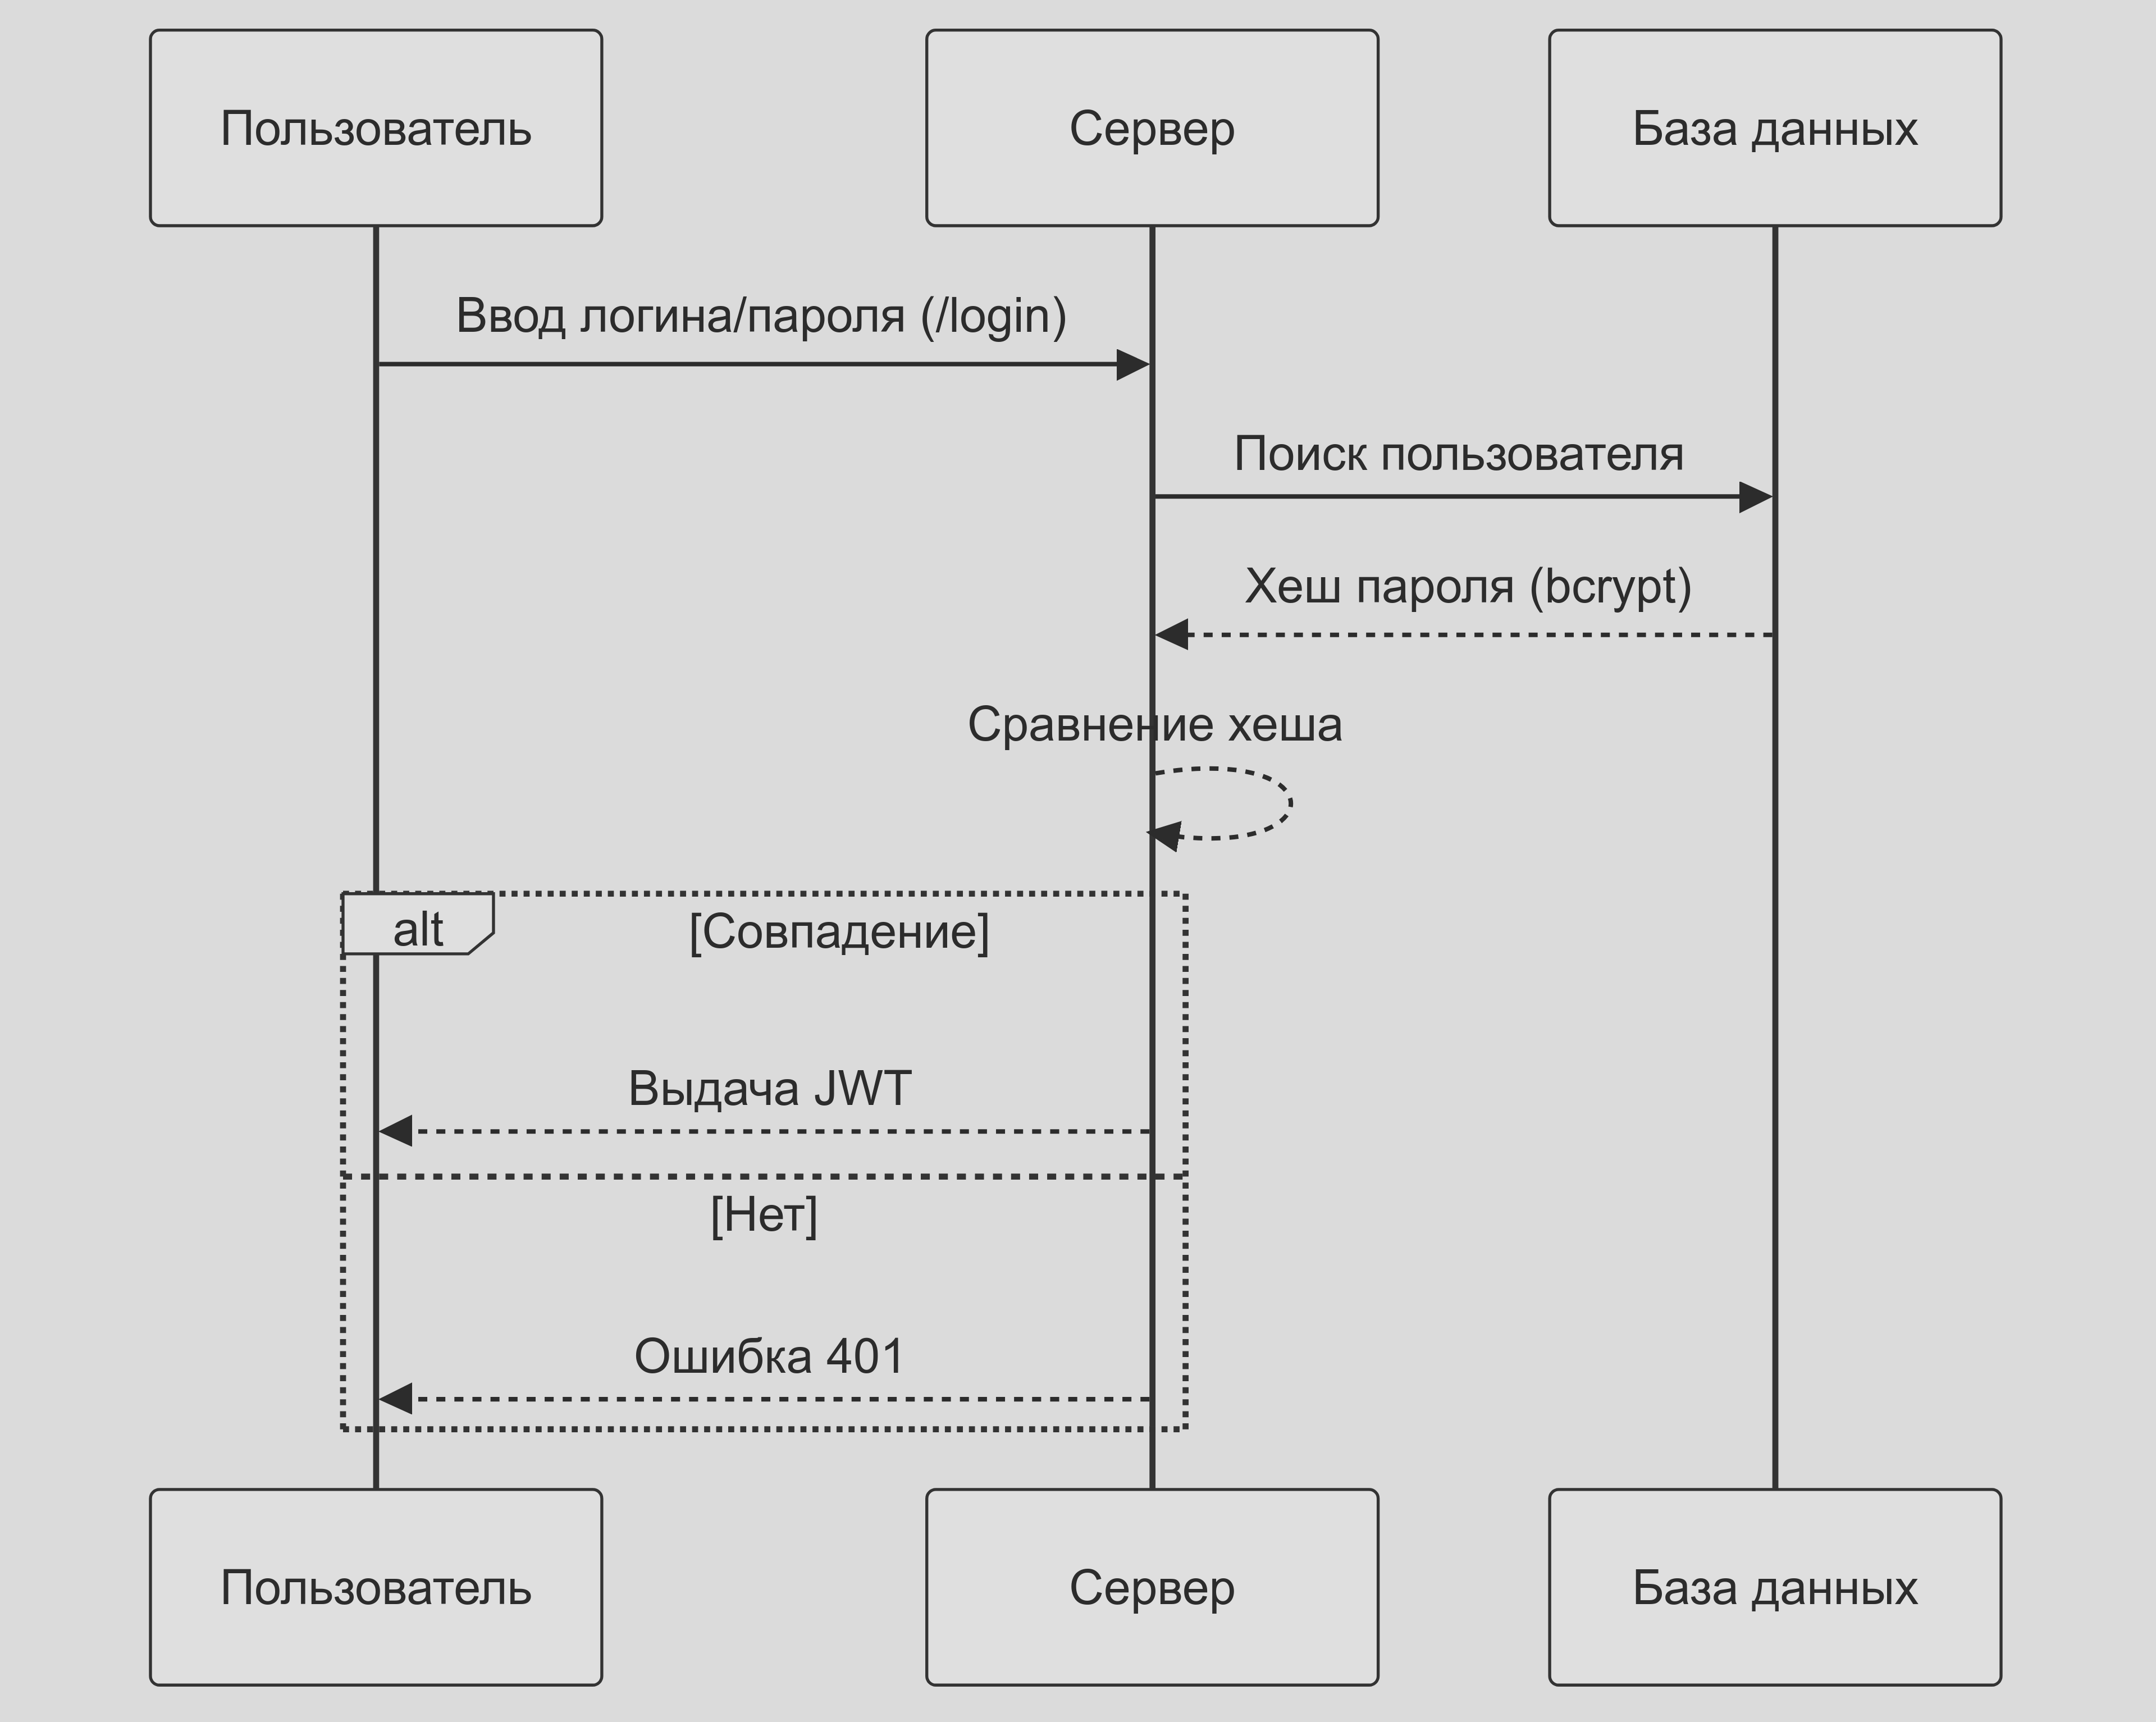
\includegraphics[width=1\textwidth]{picture/diploma-deffence-algo-1.png}
\caption{Схема аутентификации пользователя}
\label{diagram_auth}
\end{figure}


Платформа использует систему учётных записей с безопасным хранением паролей (bcrypt) и выдачей JWT-токенов. Все запросы к защищённым эндпойнтам требуют валидного JWT, что гарантирует доступ только авторизованным пользователям. Общая схема аутентификации показана на рис.~\ref{diagram_auth}.


\begin{figure}[htbp]
\centering
    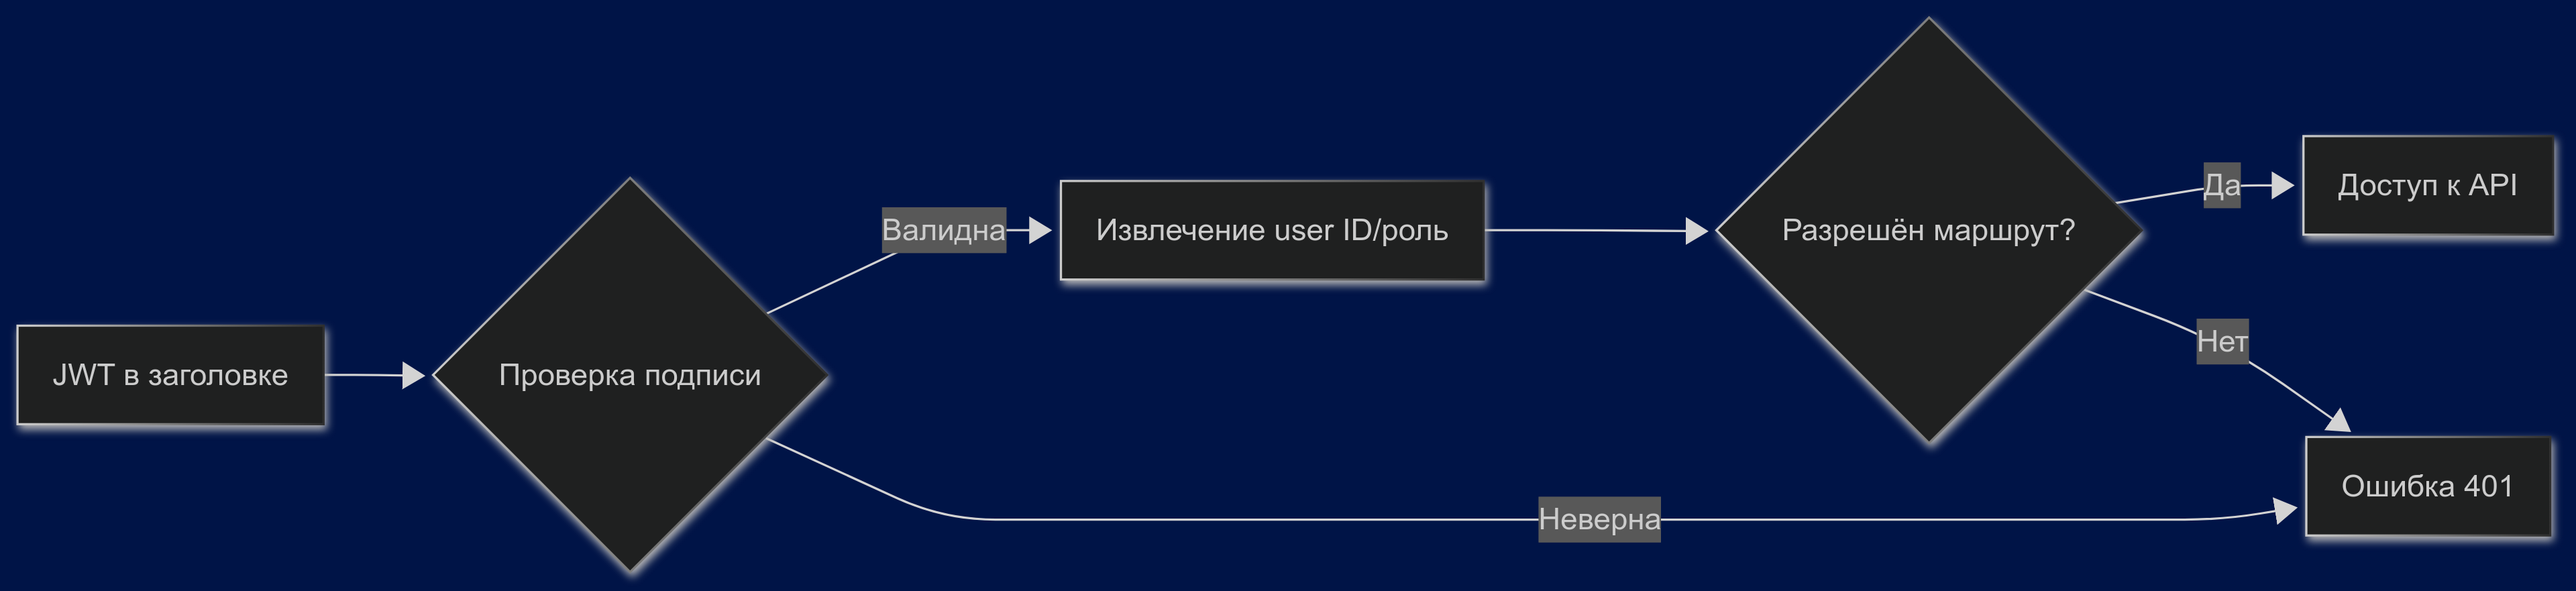
\includegraphics[width=1\textwidth]{picture/diploma-deffence-algo-2.png}
\caption{Проверка и использование JWT-токена}
\label{diagram_jwt}
\end{figure}

Разграничение доступа. На данный момент все аутентифицированные пользователи имеют одинаковые права (могут редактировать свои промпты, получать preview и т.д.). Однако система спроектирована с возможностью введения ролей. Например, можно добавить роль администратор, которому доступны дополнительные сведения (просмотр истории всех пользователей, управление учётными записями).  JWT содержит зашифрованные данные (id, роль), подписанные секретным ключом. При каждом запросе на сервер клиент прикрепляет токен в заголовке \texttt{Authorization}. Сервер валидацией подписи убеждается, что пользователь активен, и пускает к ресурсам согласно роли (рис.~\ref{diagram_jwt}).

Передача данных по сети. Взаимодействие клиент-сервер происходит по HTTP(S). Для безопасности в рабочей эксплуатации необходимо использовать протокол HTTPS с валидным SSL-сертификатом. Это гарантирует шифрование всего трафика: логинов, паролей, токенов, а также передаваемых промптов и сгенерированных результатов. Настройка HTTPS достигается либо за счёт reverse-proxy (например, Nginx с SSL передаёт на Uvicorn), либо используя встроенные возможности UVicorn + Hypercorn. Шифрование критически важно, чтобы злоумышленник в одной сети с пользователем не смог перехватить JWT-токен или крадущим образом прочесть содержимое передаваемых промптов.

Защита API и данных. Внутри серверного кода внедрены следующие меры безопасности:
\begin{itemize}
    \item шифрование (HTTPS) защищает логины, пароли и промпты;
    \item валидация данных (Pydantic) и ORM предотвращают SQL-инъекции;
    \item ключи и конфигурация (например, API-ключи) хранятся только на сервере;
    \item длина промпта ограничена (до 1000 символов), чтобы избежать злоупотреблений;
    \item история запросов и конфиденциальные данные изолированы по user\_id.
\end{itemize}

Защита данных пользователя. Помимо паролей, которые хранятся в виде хешей, следует отметить и защиту содержимого истории промптов. Хотя они не столь конфиденциальны, все же это интеллектуальная собственность пользователя (особенно для художника: удачно сформулированный промпт – ценность). Поэтому история запросов каждого пользователя закрыта от других (как описано), а также от постороннего доступа извне (невозможно без JWT вытащить эти данные через API). При хранении на диске бэкапы БД также должны быть защищены (например, шифрованы или доступны только администратору).

\paragraph{Удалённая модель и передача данных.}
DeepSeek работает как сервис «модель-как-API»: всё исполнение происходит на стороне провайдера.
Поэтому \emph{вычислительный код модели} не попадает в нашу инфраструктуру, однако
\emph{данные запроса} (промпт и контекст) передаются по сети.  
Для их защиты следует:

\begin{itemize}
  \item использовать только зашифрованные соединения (\texttt{https});
  \item хранить ключ доступа (\texttt{DEEPSEEK\_API\_KEY}) в \texttt{.env} и передавать в заголовке \texttt{Authorization: Bearer};
  \item регулярно ротировать ключ и немедленно отзывать его при подозрении на компрометацию.
\end{itemize}

\paragraph{Prompt-injection и нежелательный контент.}
Даже будучи удалённой, модель остаётся уязвимой к \emph{prompt injection}: злоумышленник может сформулировать
вопрос так, чтобы обойти системные инструкции и получить приватные данные или токсичный текст.
Чтобы смягчить риск, применяются два уровня фильтрации:

\begin{enumerate}[label=\arabic*]
  \item \textbf{Фильтр провайдера.} DeepSeek имеет встроенную модерацию и блокирует ответы, нарушающие правила использования.
  \item \textbf{Локальная пост-обработка.}  На стороне сервера можно
        \begin{itemize}
          \item проверять результат на стоп-слова/регулярные выражения,
          \item прогонять его через open-source «модератор»-модель,
          \item при необходимости усекать длину или удалять чувствительные данные перед отправкой клиенту.
        \end{itemize}
\end{enumerate}

\paragraph{Обновления безопасности.}
Клиентское ПО (\texttt{requests}, SDK DeepSeek, FastAPI) и базовый контейнер
нужно регулярно обновлять, так как в них могут обнаруживаться уязвимости.
Использование Docker облегчает переход на новые безопасные образы ОС.
Кроме того, при смене \texttt{DEEPSEEK\_API\_KEY} старые JWT-токены автоматически устаревают,
что защищает от повторного использования скомпрометированных ключей.

Таким образом, при обращении к DeepSeek мы переносим вычислительную нагрузку
с локального GPU на облако, но должны уделить больше внимания защите канала связи,
управлению ключами и пост-фильтрации содержимого \cite{deepseek:docs}.

Безопасность инфраструктуры. Сервер, на котором размещается система, должен быть защищен: настроен файрвол (открыты только необходимые порты – 443 для HTTPS, 80 может редиректиться на 443, и, возможно, 22 для SSH админа). Доступ к серверу по SSH – только администратору с ключом, либо через VPN. PostgreSQL сервер, если отдельный, то либо локальный, либо за firewall – не в открытом интернет (или по крайней мере с ограничением по IP доступа до сервера приложения). Резервные копии БД следует хранить шифрованно, если хранятся вне сервера.

Подытоживая: аутентификация в системе реализована посредством логина/пароля с безопасным хранением (bcrypt-хеши) и выдачей JWT-токенов. Авторизация (проверка прав) – все основные маршруты требуют валидного токена, и пользователь имеет доступ только к своим данным. Безопасность данных и кодов обеспечивается на нескольких уровнях: шифрование канала (HTTPS), валидация входа, защита БД от инъекций, ограничение привилегий. Принятые меры соответствуют общепринятым практикам веб-безопасности (OWASP) и учитывают особенности нашей платформы (включая интеграцию ML). Таким образом, система защищена от большинства распространённых угроз: утечки учётных данных, несанкционированного доступа к данным, перехвата трафика, SQL-инъекций, brute-force атак на пароли и др. Это создаёт прочную основу доверия для пользователей: они могут безопасно использовать платформу, не опасаясь за сохранность своих персональных данных и уникальных промптов.
\subsection{Вывод}
В разделе проектирования была разработана подробная архитектура и техническое решение для платформы интерактивного формирования, оценки и предварительного просмотра запросов (промптов) к языковым и генеративным нейросетям. Платформа построена по принципу клиент-сервер и включает серверное приложение на FastAPI, взаимодействующее с внешними API Fusion Brain (модель Kandinsky 3.1) и DeepSeek для генерации изображений и текста, веб-клиент на Vue.js для удобного интерфейса и базу данных PostgreSQL для хранения пользовательских данных.

На основании требований были спроектированы конкретные методики реализации всех заявленных функций: редактирование промптов как в текстовом режиме, так и путём перетаскивания токенов; автоматизированное дополнение описаний с использованием возможностей большой языковой модели; вычисление метрики качества промпта по набору правил; преобразование формата запросов под требования разных моделей; механизм preview, позволяющий быстро получать отклики от модели (текстовые – через DeepSeek, графические – через FusionBrain) и показывать их пользователю. Каждый из этих функциональных блоков был рассмотрен с точки зрения алгоритмов и программных средств, что показало реализуемость поставленных задач.

Разработанная архитектура системы демонстрирует баланс между использованием локальных ресурсов и облачных сервисов: тяжёлая языковая модель размещена локально, что даёт независимость от внешних API и быстрый отклик, тогда как генерация изображений делегирована специализированному удалённому сервису для достижения высокого качества без чрезмерных требований к оборудованию. Клиентское приложение на Vue.js обеспечивает интерактивность и отзывчивый интерфейс, удовлетворяющий потребностям как технических, так и творческих пользователей.

В ходе проектирования были приняты обоснованные схемотехнические, алгоритмические, программные и конструктивно-технологические решения. Выбор FastAPI и PyTorch на сервере обеспечил высокую производительность и гибкость при интеграции ML-модели, выбор Vue.js на клиенте – удобство реализации сложного UI. Внедрение JWT-аутентификации, bcrypt-хеширования паролей и других мер безопасности позволило создать надежный механизм защиты данных, что немаловажно для приложения, работающего с пользовательским контентом.

Проектирование учитывало профиль пользователей системы (разработчики и художники) – в решениях особое внимание уделено удобству интерфейса (двойной режим редактирования, визуальный просмотр результатов), а также обеспечению того, чтобы ни одна из групп не была технически ограничена в использовании платформы. Все требования заказчика по функционалу удовлетворены предлагаемым дизайном: система позволяет интерактивно экспериментировать с промптами, улучшать их качество и сразу видеть, к чему эти улучшения приводят, что в конечном итоге повышает эффективность работы с нейросетевыми моделями.


\section{Реализация платформы для интерактивного формирования запросов к языковым и генеративным нейросетям}

В данном разделе подробно описывается реализация программной платформы, предназначенной для интерактивного формирования запросов к современным языковым моделям и генеративным нейросетям. Целью разработки было создать удобный и гибкий инструмент, позволяющий пользователям составлять сложные запросы к моделям искусственного интеллекта (как текстовым, так и визуальным) в интерактивном режиме, используя наглядный интерфейс. Такой подход упрощает работу с крупными языковыми моделями и генеративными моделями изображений, скрывая сложность формулировки \textit{prompt}'ов \cite{lakera:2025} (текстовых запросов) и последовательной обработки данных.

Разрабатываемая платформа реализована по архитектуре клиент--сервер: \textbf{frontend} (клиентское веб-приложение) создан на основе Vue 3 с использованием хранилища состояний Pinia, а \textbf{backend} (серверная часть) реализован на фреймворке FastAPI на языке Python\cite{fastapi:practicum}. В качестве базы данных используется PostgreSQL с подключённым расширением pgvector для хранения и поиска векторных представлений данных. Данный стек технологий был выбран с учётом требований к интерактивности интерфейса, необходимости вызывать внешние API генеративных моделей, а также для обеспечения возможности масштабирования и расширения функциональности.

Ниже приводится структурированное описание архитектуры системы и ключевых компонентов реализации. Сначала рассматривается общая архитектура платформы и взаимодействие между её компонентами. Затем описывается клиентская часть, в том числе реализация drag-and-drop интерфейса для формирования запросов. После этого подробно изложена работа серверной части: обработка запросов, интеграция с внешними API (для генерации текстов и изображений) и использование векторного поиска для улучшения качества результатов. Завершает раздел \textbf{вывод} с описанием достигнутых результатов разработки и перспектив расширения системы.

\subsection{Архитектура платформы}

Разработанная платформа имеет многоуровневую архитектуру, разделяя функциональность между клиентской и серверной частями. На рис.~\ref{architecture} схематично представлено взаимодействие основных компонентов системы. Клиентское приложение предоставляет интерфейс пользователю для формирования запроса и визуализации результатов, в то время как серверное приложение отвечает за обработку этого запроса, взаимодействие с внешними сервисами (генеративными моделями) и доступ к базе данных. Такой подход соответствует принципам разделения ответственности и упрощает поддержку и модификацию системы.

Основные компоненты архитектуры:
\begin{enumerate}[label=\arabic*]
\item \textbf{Интерфейс пользователя (Frontend, Vue 3 + Pinia):} Одностраничное веб-приложение (single-page application), работающее в браузере. Отвечает за отображение элементов интерфейса, сбор ввода пользователя и интерактивное формирование запросов. Использование Vue 3 обеспечивает реактивность интерфейса и модульность кода, а Pinia используется для централизованного управления состоянием приложения (например, текущим набором элементов запроса, история запросов и результатов и др.)\cite{vuejs:wiki}.
\item \textbf{Сервер приложений (Backend, FastAPI):} Веб-сервер, реализующий API для обработки запросов от фронтенда. На сервере реализована бизнес-логика: получение структурированного запроса пользователя, его возможная предобработка (например, добавление контекста из базы знаний), вызов внешних API генеративных моделей для выполнения запроса (например, генерация текста или изображения), постобработка полученного результата и возврат ответа клиентскому приложению. Благодаря фреймворку FastAPI обеспечивается высокая производительность и поддержка асинхронной обработки, что особенно важно при параллельных запросах к внешним сервисам \cite{yandex:fastapi}.
\item \textbf{База данных (PostgreSQL + pgvector):} Хранилище данных, используемое платформой для сохранения необходимой информации. Реляционная СУБД PostgreSQL выбрана за её надёжность и масштабируемость, а расширение pgvector позволяет хранить эмбеддинги (векторные представления) текстовых данных и выполнять поиск по схожести этих векторов \cite{postgresql:wiki}. База данных может сохранять, например, историю диалогов, сгенерированные ответы, либо набор справочных данных (знаний), которые используются моделью для более осмысленных ответов. Посредством pgvector реализован семантический поиск: по входному запросу можно находить ближайшие по смыслу тексты и подставлять их в качестве контекста для языковой модели.
\item \textbf{Внешние AI-сервисы:} Генеративные модели, с которыми взаимодействует платформа, развернуты на внешних серверах и доступны через API. Для генерации текста используется модель DeepSeek R1 (предоставляемая через DeepSeek API)\cite{deepseek:docs}, а для генерации изображений --- модель диффузионного типа (Kandinsy) через соответствующий API\cite{sitelabs:kandinsky}. Оба типа моделей являются современными представителями генеративных нейросетей: DeepSeek R1 — крупная языковая модель с поддержкой диалога и глубокого рассуждения, Kandinsky — модель для синтеза изображений по текстовому описанию. Обращение к ним по API означает, что вычислительные ресурсы по генерации выделены на стороне сервиса, а наша платформа выступает как посредник, отправляющий запросы и получающий готовые результаты.
\end{enumerate}

Взаимодействие компонентов происходит по следующему сценарию. Пользователь посредством фронтенда формирует запрос (например, текстовое описание задачи или сцены для генерации изображения). При отправке запроса клиентское приложение собирает все необходимые данные (включая текстовые поля, выбранные опции, прикреплённые изображения или другие элементы) и отправляет их на сервер через HTTP-запрос к API. Серверная часть принимает запрос, анализирует его тип и содержимое: если требуется текстовая генерация, вызывается соответствующий метод, если генерация изображения — другой метод. Перед обращением к модели сервер может обратиться к базе знаний: например, выполнить векторный поиск по базе ранее сохранённых данных для нахождения дополнительного контекста (релевантных текстов) и объединить их с запросом пользователя. Затем сервер формирует запрос к внешнему API нужной модели (с учётом ключа доступа и формата, требуемого API), и ожидает ответа. Получив результат от модели (сгенерированный текст или изображение), сервер производит сохранение результата в базу (при необходимости) и возвращает результат клиенту. Фронтенд, получив ответ, отображает пользователю сгенерированный контент. В случае изображения оно выводится прямо на страницу, в случае текста — отображается в виде ответа ассистента. При этом интерфейс может позволять пользователю далее уточнять запрос (например, задать уточняющий вопрос или отредактировать сгенерированный результат и отправить повторно), образуя интерактивный цикл работы.

Подобная архитектура обеспечивает гибкость: компоненты чётко разделены, что даёт возможность модифицировать их независимо. Например, можно заменить модель генерации текста на другую, не затрагивая интерфейс, достаточно изменить вызов в серверной части. Или можно развивать фронтенд (добавлять новые элементы взаимодействия) без изменения логики генерации на сервере. Использование стандартных веб-технологий (HTTP API, JSON) для обмена данными между фронтендом и бэкендом обеспечивает совместимость и простоту отладки.

\subsection{Интерфейс с перетаскиванием элементов (Frontend на Vue 3 + Pinia)}

Клиентская часть платформы реализована как одностраничное приложение на Vue 3, что позволяет создать динамичный интерфейс, обновляющийся без полной перезагрузки страницы. Одной из ключевых задач фронтенда было обеспечить \textit{drag-and-drop} интерфейс для интерактивного составления запросов. Это означает, что пользователю предоставляется возможность добавлять, удалять и менять местами различные блоки запроса с помощью мыши, просто перетаскивая элементы на экране.

Для реализации drag-and-drop функциональности были использованы возможности HTML5 Drag and Drop API и компоненты Vue. В частности, элементы интерфейса, представляющие части запроса (например, фрагмент текста инструкции, блок для ввода вопроса, изображение-пример или параметры генерации), сделали перетаскиваемыми с помощью атрибутов \verb|draggable| и соответствующих обработчиков событий (\verb|dragstart|, \verb|dragover|, \verb|drop| и т.д.). Когда пользователь начинает перетаскивание элемента, приложение запоминает (через Pinia-хранилище) текущий переносимый объект. Когда происходит сброс (drop) элемента на новую позицию или область, обновляется состояние списка блоков запроса. Pinia отвечает за централизованное хранение структуры запроса: каждый блок может быть представлен объектом с полями, описывающими его тип (текст, изображение, параметр), содержимое (например, сам текст или ссылка на файл изображения) и, возможно, дополнительные настройки.

Благодаря реактивности Vue, обновление состояния Pinia автоматически приводит к перерисовке списка блоков на экране в новом порядке. Это даёт плавный пользовательский опыт при сборке запроса из блоков. Пользователь может, к примеру, перетащить в область запроса готовый шаблон подсказки (prompt template)\cite{copilotworks:promptgen} из библиотеки слева, затем добавить свои уточнения текстом, а затем перетянуть специальный блок, обозначающий место, куда будет подставлен результат другого запроса. Такой механизм особенно полезен для составления сложных запросов, например, когда требуется сгенерировать текст по определённому шаблону или выполнить несколько шагов генерации (сначала текст, потом на основе этого текста — изображение).

Стоит отметить, что Pinia значительно упростила реализацию управления состоянием по сравнению с классическим Vuex (Vue 2), благодаря более простому синтаксису и TypeScript-совместимости. Были созданы отдельные store (хранилища) Pinia для разных частей состояния приложения. Например, один store хранит текущий состав блоков запроса (их список и свойства), другой — историю предыдущих запросов и ответов, третий — настройки пользователя (выбранные модели генерации, параметры вроде температуры генерации текста, желаемого разрешения изображения и т.п.). Разделение на несколько хранилищ повышает модульность: логика по управлению историей отделена от логики формирования текущего запроса.

Ниже приведён упрощённый пример компонента Vue, реализующего область с перетаскиваемыми блоками запроса. В этом фрагменте кода показано, как можно выводить список блоков и обеспечивать их перетаскивание с помощью директивы \verb|v-for| и событий drag-and-drop:

\begin{lstlisting}[language=HTML]
       <div class="query-builder" @drop="onDrop" @dragover.prevent>
             <div class="query-block" v-for="(block, index) in blocks" :key="block.id" draggable="true" @dragstart="onDragStart(block, index)">
               <div v-if="block.type === 'text'"> {{ block.text }} </div> <div v-else-if="block.type === 'image'">
                <img :src="block.preview" alt="Image" /> </div> <div v-else-if="block.type === 'param'">
                 <span>{{ block.name }}: {{ block.value }}</span>
                </div>
                </div>
              </div>
\end{lstlisting}

\vspace{-0.5\baselineskip} 
В приведённом фрагменте шаблона Vue каждый элемент \verb|<div class="query-block">| представляет отдельный блок запроса, который может быть текстовым, изображением или блоком параметров. Атрибут \verb|draggable="true"| делает элемент перетаскиваемым. Обработчик \verb|@dragstart| привязан к методу \verb|onDragStart|, который сохраняет переносимый блок и его индекс. Обработчик \verb|@drop| на контейнере \verb|query-builder| вызывается, когда блок отпущен в новой позиции; внутри метода \verb|onDrop| происходит обновление порядка блоков в списке \verb|blocks|. Использование \verb|@dragover.prevent| необходимо, чтобы разрешить сброс элементов (по умолчанию браузер запрещает сброс для необработанных зон). Таким образом, этот компонент даёт возможность динамически менять состав и последовательность частей запроса.

Другой важной частью фронтенда является форма ввода и отображения результатов. Над областью сборки запроса размещены поля для ввода основного текста запроса пользователя, а также (опционально) для указания негативных подсказок (\textit{negative prompt} для генерации изображений, чтобы исключить нежелательные детали), выбора модели или пресета настроек. Рядом располагаются кнопки: "Сгенерировать текст", "Сгенерировать изображение" и т.п., в зависимости от выбранного типа задачи. После нажатия соответствующей кнопки собранная структура запроса отправляется на сервер.
\begin{figure}[htbp]
    \centering
    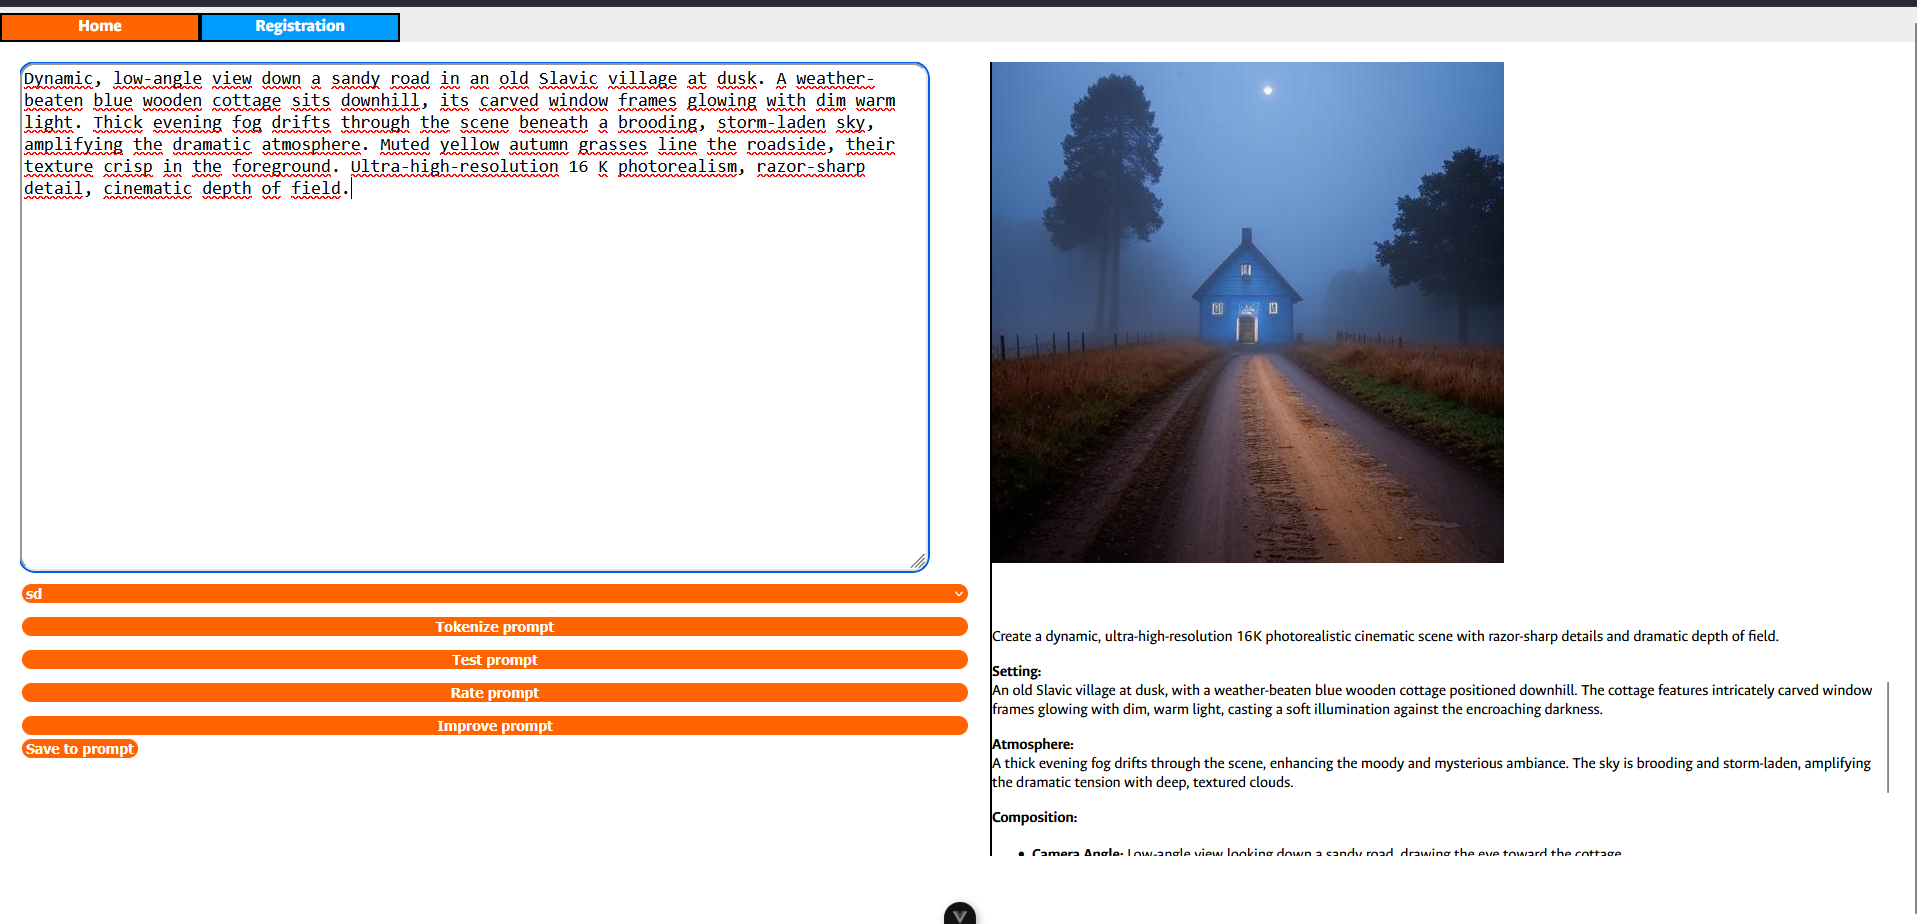
\includegraphics[width=0.8\textwidth]{picture/interface-screenshot_1.png}
    \caption{Алгоритм оценки качества запроса}\label{interface-screenshot}
\end{figure}
Для отображения результатов на странице предусмотрены соответствующие области: текстовые результаты показываются в виде ленты с историей запросов что можно увидеть на рисунке \ref{interface-screenshot}, изображения — в виде изображений в истории запросов. Все эти элементы также управляются состоянием Pinia: результат генерации (например, полученный от модели текст) сохраняется в историю запросов и отображается вместе с исходным запросом.

Таким образом, frontend обеспечивает интерактивное и наглядное взаимодействие: пользователь манипулирует блоками запроса и сразу видит, как формируется итоговый запрос, а после отправки — мгновенно получает отображение результата. Высокая отзывчивость интерфейса достигается благодаря возможностям Vue 3 по оптимизации обновлений DOM и использованию reactive-переменных, а также благодаря разгрузке тяжёлых вычислений на backend и внешние сервисы.

\subsection{Серверная часть и интеграция с внешними API (Backend на FastAPI)}

Серверное приложение, реализованное на FastAPI, отвечает за приём запросов от фронтенда, их обработку и взаимодействие с моделями ИИ через внешние API. FastAPI был выбран по нескольким причинам: во-первых, он обеспечивает высокую производительность и низкую задержку благодаря использованию асинхронного подхода (на базе UVicorn/Starlette); во-вторых, имеет удобный механизм автоматической генерации документации API (OpenAPI/Swagger), что упрощает отладку и тестирование; в-третьих, написан на Python, что облегчает интеграцию с Python-библиотеками для машинного обучения и вызова внешних API.

На стороне backend определён набор REST API-эндпоинтов, соответствующих различным функциям платформы. Основные из них:
\begin{enumerate}[label=\arabic*]
\item \verb|GET /tokenize-prompt| -- принимает строку \verb|prompt| (дефисы автоматически заменяются на пробелы), разбивает её при помощи \verb|PromptTokenizer| и возвращает структурированное представление (\verb|PromptStructure|) для дальнейшей работы фронтенда с токенами и тегами.

\item \verb|GET /rate-prompt| -- принимает строку \verb|prompt| и тип модели (\verb|model|, см. enum \verb|InputTypes|), вычисляет «оценку качества» промпта через \verb|PromptRatingHandler| и возвращает числовой/категориальный рейтинг.

\item \verb|GET /preview-image| -- запускает генерацию изображения в FusionBrain\cite{fusionbrain:docs} (получает \verb|pipeline_id|, генерирует, циклически опрашивает до готовности) и отдаёт результат как \verb|StreamingResponse| с \verb|image/jpeg|. Параметр запроса: \verb|prompt|.

\item \verb|GET /preview-text| -- пробный прогон текста через LLM (\verb|DeepSeekTestService|): принимает \verb|prompt| и асинхронно возвращает ответ модели (строка или JSON с сообщением).

\item \verb|GET /improve-prompt| -- улучшает текстовый промпт с помощью \verb|DeepSeekTestService|: принимает \verb|prompt| и возвращает переработанную, более детальную или уточнённую команду для текстовой модели.

\item \verb|GET /extend-image-prompt| -- расширяет/улучшает промпт для генерации изображений (также через \verb|DeepSeekTestService|): принимает \verb|prompt| и отдаёт дополненный промпт, включающий дополнительные стилистические детали или ключевые слова.
\end{enumerate}

Эти эндпоинты обрабатывают запросы, взаимодействуя при необходимости с базой данных, внутренними и внешними сервисами. Приведём блок-схему алгоритма внутреннего сервиса, иллюстрирующий принципы работы сервиса оценки качества запросов платформы. Он принимает данные запроса, отправляет его на сервис классификации и полученный объект проверяет на соответствие пропорциям согласно выбранной модели и в зависимости от степени соответствия выставляется рейтинг:

\begin{figure}[htbp]
    \centering
    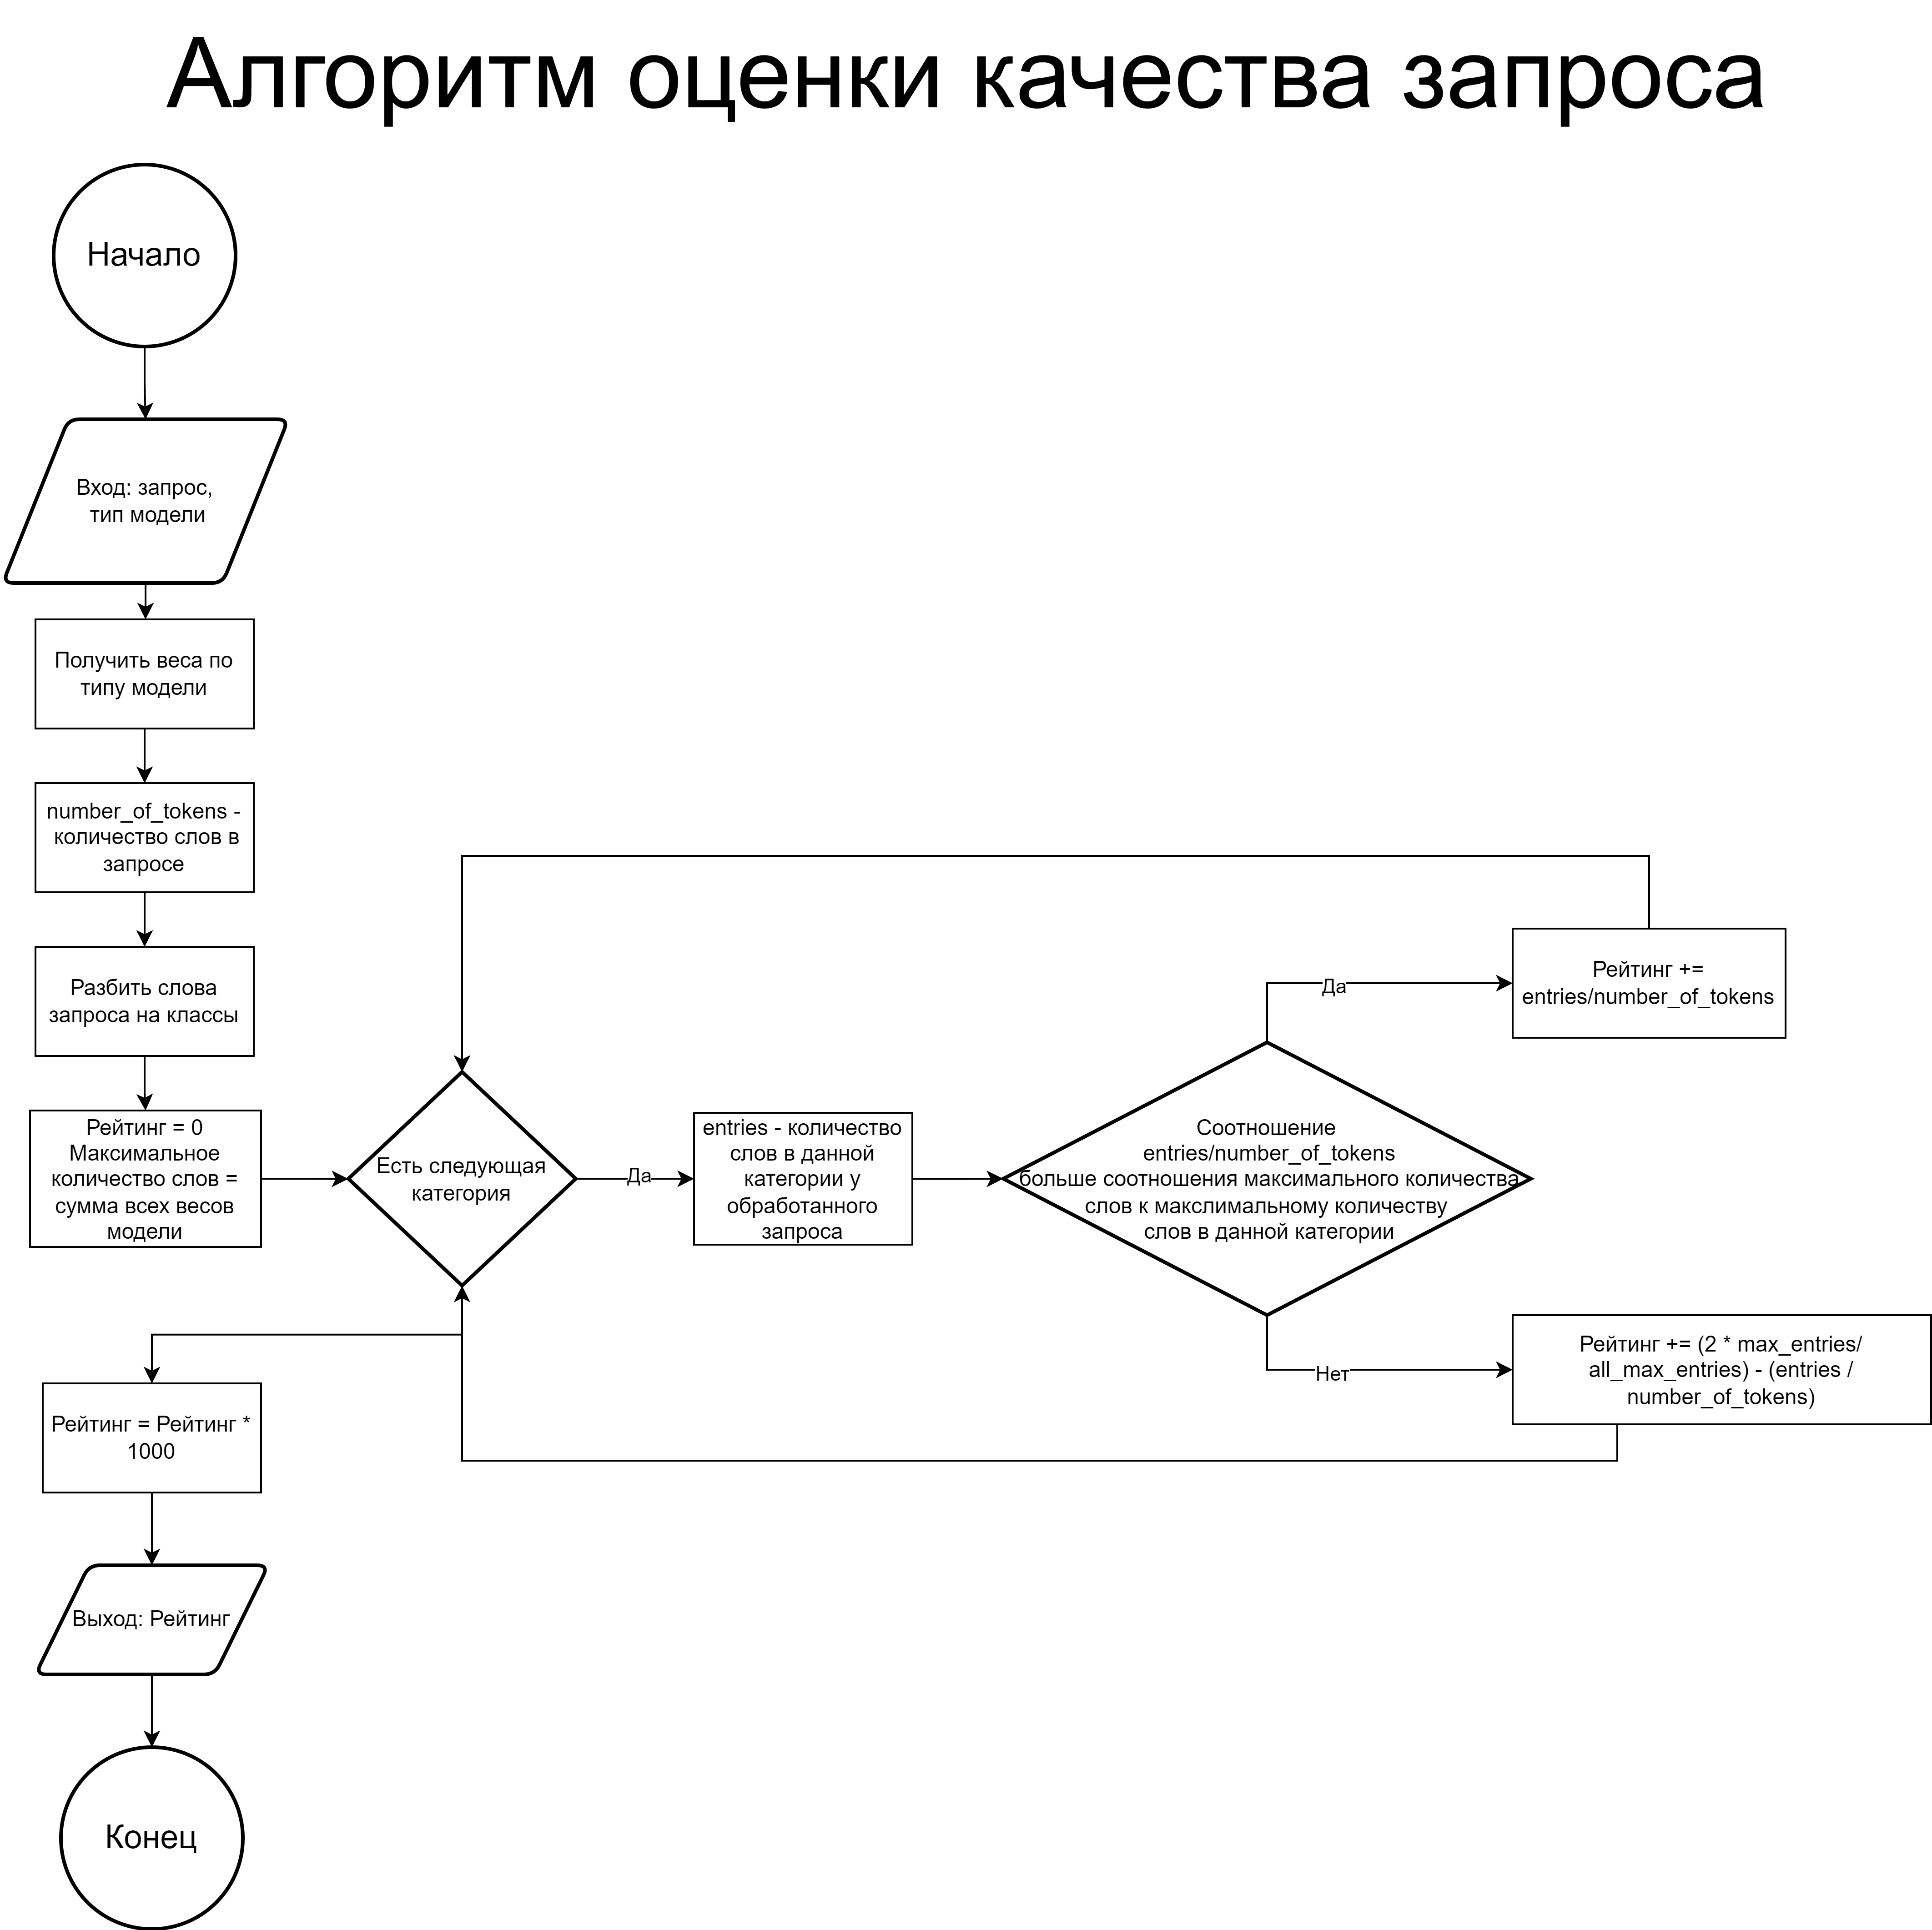
\includegraphics[width=0.8\textwidth]{picture/rating-algoritm.png}
    \caption{Алгоритм оценки качества запроса}
    \label{rating-algoritm}
\end{figure}

Как можно заметить на диаграмме \ref{rating-algoritm}, алгоритм оценки качества запроса обращается к сервису тематической классификации промптов.  
Ниже приведено описание его работы.

\subsubsection*{Алгоритм тематической классификации токенов}

\begin{enumerate}[label=\arabic*]
  \item \textbf{Предобработка и токенизация.}  
        Исходная строка запроса переводится в нижний регистр, после чего
        разбивается на токены методом \verb|word_tokenize| из пакета NLTK.
  \item \textbf{Очистка от «семантически лёгких» слов.}  
        Из полученного списка исключаются все знаки пунктуации и стоп-слова
        (англоязычный список \verb|stopwords| из NLTK), поскольку они
        не несут предметной нагрузки в задаче оценки творческого промпта.
  \item \textbf{Часть-речи-теггинг с универсальным набором тегов.}  
        Каждый оставшийся токен маркируется тэгами
        \texttt{NOUN}, \texttt{VERB}, \texttt{ADJ}, \texttt{ADV} и т.д.
        (\verb|nltk.pos_tag(..., tagset="universal")|) – это даёт
        начальное распределение признаков по грамматическим ролям.
  \item \textbf{Приведение POS-тегов к формату WordNet.}  
        Функция \verb|_nltk_to_wordnet| отображает универсальные теги
        в четыре базовые категории WordNet: \texttt{NOUN}, \texttt{VERB},
        \texttt{ADJ}, \texttt{ADV}. Это необходимо для корректной
        лемматизации и поиска синонимов.
  \item \textbf{Лемматизация.}  
        Каждый токен \(\,w_i\) заменяется своей леммой
        \(l_i=\mathrm{lemma}(w_i,\mathrm{POS}_i)\) с помощью
        \verb|WordNetLemmatizer|. Лемматизация уменьшает
        размер словаря и упрощает последующее семантическое сравнение.
  \item \textbf{Формирование базовых синонимических множеств.}  
        Для каждой из восьми категорий  
        \(\mathcal{C}=\{\text{clarity},\text{descriptive},\ldots,\text{negative}\}\)
        задаётся набор лемматизированных ключей
        \(K_c=\{k_{c,1},k_{c,2},\ldots\}\).
        Эти множества предварительно тегированы и хранятся в памяти
        (\verb|self.lemmatized_keywords|).
  \item \textbf{Семантическая близость «токен – ключ».}  
        Для каждой пары «токен» \(l_i\) и «ключ» \(k_{c,j}\) с совпадающим
        POS вычисляется мера Ликока–Чодоровa  
        \[
          S(l_i,k_{c,j})=\operatorname{lch\_similarity}
          \bigl(\operatorname{synset}(l_i),\operatorname{synset}(k_{c,j})\bigr).
        \]  
        Максимальное значение  
        \(S_{\text{max}}(l_i)=\max_{c,j}S(l_i,k_{c,j})\)
        определяет категорию \(c^\star\) с наибольшей
        семантической связанностью.
  \item \textbf{Назначение категории и агрегация результата.}  
        Токен \(l_i\) помещается в подмножество
        \(R_{c^\star}\subseteq\mathcal{R}\), где
        \(\mathcal{R}=\{R_{\text{clarity}},\ldots,R_{\text{negative}}\}\) —
        итоговая структура данных, возвращаемая методом
        \verb|tokenize_prompt| в формате  
        \verb|{"clarity": [...], "descriptive": [...], ...}|.
\end{enumerate}

\paragraph{Комплексная оценка.}
Полученный словарь категорий служит входом для последующих
метрик качества: каждая из восьми компонент оценивается
взвешенным числом релевантных токенов и
передаётся в «оценщик» \verb|PromptRatingHandler|.
Таким образом, классификатор выполняет роль
семантического препроцессора, переводя
сырой текстовый ввод в компактное многоканальное
представление, пригодное для детализации промпта,
выделения слабых мест и формирования
пользовательских рекомендаций.

\paragraph{Ключевые отличия относительно «черновика».}
\begin{itemize}
  \item Используется \textbf{POST}-запрос с валидацией входных данных через
        \verb|pydantic|-модель \verb|ImageGenerationRequest|.
  \item В качестве генератора изображений выступает \texttt{FusionBrainAPI},
        а не абстрактный «Stable Diffusion» по фиксированному URL; это устраняет
        дублирование конфигурации и позволяет изменять провайдера без правки
        эндпоинта.
  \item Параметр \verb|steps| пока не поддерживается FusionBrain, 
        но оставлен как поле запроса — при появлении соответствующей функции
        он автоматически «пройдёт» сквозь интерфейс.
  \item Возврат осуществляется \emph{всегда} в виде строки Base64
        (\verb|"image_base64"|), что упрощает работу фронтенда в SPA-приложении:
        достаточно создать тег
        \verb|<img src="data:image/png;base64,{{image_base64}}">|.
\end{itemize}

Таким образом, эндпоинт полностью согласован с предоставленными классами
\texttt{FusionBrainAPI} и унифицирован со схемой остальных маршрутов сервиса.

Приведённые обработчики демонстрируют принцип интеграции с внешними API: наш сервер выступает прокси, перекладывая запрос пользователя на внешний сервис генерации контента. Разумеется, в реальном приложении необходимо учитывать ряд дополнительных аспектов:
\begin{enumerate}[label=\arabic*]
\item Асинхронная обработка: вызовы \verb|requests.post| к внешним сервисам могут занимать значительное время (сотни миллисекунд или несколько секунд). Чтобы не блокировать event loop FastAPI, можно использовать асинхронные HTTP-клиенты (например, \verb|httpx|) или выносить подобные вызовы в \verb|run_in_threadpool|. Это позволит обрабатывать несколько запросов параллельно и лучше использовать ресурсы сервера.
\item Обработка ошибок и повторные попытки: внешний сервис может быть недоступен или вернуть ошибку (как учтено в коде через \verb|HTTPException|). Дополнительно можно реализовать логику повторного запроса (retry) с экспоненциальной задержкой, логирование ошибок для последующего анализа и вывода информативного сообщения пользователю (например, "Сервис генерации временно недоступен, попробуйте позже").
\item Безопасность и хранение ключей: строка \verb|API_KEY| в коде хранит секретный ключ доступа к API. В реальном проекте его следует загружать из защищённых настроек (например, переменных окружения или конфигурационного файла, не хранящегося в репозитории) и не раскрывать на стороне клиента. Наш backend скрывает этот ключ, выступая посредником — фронтенд не обращается напрямую к внешним API, чтобы не экспонировать ключ в браузере.
\item Формат ответа и постобработка: для текстовой модели DeepSeek может потребоваться обработка разметки (если модель возвращает ответ с Markdown или особыми токенами), для изображений — возможно сохранение файла на сервере и отдача ссылки вместо передачи большого base64 прямо (для экономии трафика). В нашем прототипе мы передаём base64-строку для простоты.
\end{enumerate}

Backend также осуществляет сохранение результатов и данных в базу PostgreSQL. Например, после успешной генерации текста можно сохранить сам запрос пользователя, полученный ответ и некоторую мета-информацию (время, используемую модель) в таблицу \verb|queries| для последующего анализа или отображения истории на фронтенде. Аналогично, для изображений можно сохранять URL или путь к файлу сгенерированного изображения, чтобы не потерять его при обновлении страницы. Однако хранение изображений непосредственно в базе (в виде байтов или base64) неэффективно; лучше сохранять файл на диске или облачном хранилище, а в базе держать ссылку.

Для организации доступа к базе данных сервер использует либо ORM (например, SQLAlchemy) либо простой драйвер (psycopg2) для выполнения SQL-запросов. В нашем случае, учитывая необходимость работы с pgvector, можно выполнять SQL напрямую для большей прозрачности. Рассмотрим следующий аспект подробнее.

\subsection{Реализация векторного поиска (PostgreSQL + pgvector)}

Одной из особенностей платформы является использование \emph{векторного поиска}
для повышения качества ответов и удобства пользователя.
Векторное представление текста позволяет находить семантически близкие фрагменты,
а не лишь лексические совпадения.  
Тексты кодируются в эмбеддинги фиксированной размерности
(в дипломном проекте – $384$-мерные эмбеддинги  
модели \verb|sentence-transformers/all-MiniLM-L6-v2|),
после чего метрика близости (косинусное расстояние) применяется непосредственно в базе данных\cite{wiki:cosine_similarity}.

\paragraph{Сценарии применения.}
\begin{enumerate}[label=\arabic*]
  \item \textbf{Дополнение запросов внешним контекстом.}  
        Перед генерацией ответа LLM формируется эмбеддинг пользовательского запроса,
        выполняется поиск в коллекции справочных документов
        и $k$-наиболее близких абзацев передаются модели в качестве
        системного контекста (RAG-подход).
  \item \textbf{Семантический поиск по истории.}  
        Каждый факт взаимодействия (\texttt{TestHistory}) снабжается эмбеддингом.
        Пользователь может быстро найти прошлые диалоги «по смыслу».
  \item \textbf{Рекомендация похожих запросов.}  
        На этапе ввода запроса клиенту можно предлагать примеры из общей базы, вычисляя ближайшие эмбеддинги «на лету»\cite{flowgpt:community}.
\end{enumerate}

\paragraph{Структура таблиц.}
Для хранения эмбеддингов PostgreSQL расширяется модулем \texttt{pgvector}:

\begin{lstlisting}
      
CREATE EXTENSION IF NOT EXISTS pgvector;

CREATE TABLE documents (
  id         BIGINT PRIMARY KEY GENERATED ALWAYS AS IDENTITY,
  source_id  TEXT NOT NULL,
  embedding  VECTOR(384) NOT NULL
);

CREATE INDEX ON documents
USING hnsw (embedding vector_l2_ops)
WITH (m = 16, ef_construction = 200);
\end{lstlisting}


\paragraph{Пример SQL-запроса.}
Оператор \verb|::vector| приводит JSON-массив к типу \texttt{VECTOR}\@.
Для косинусной близости в \texttt{pgvector 0.5+}
используется оператор \verb|<=>|:

\begin{lstlisting}[language=SQL]
SELECT id, source_id,
       embedding <=> '[0.12, 0.34, ..., 0.88]'::vector AS distance
FROM   documents
ORDER  BY distance                               
LIMIT  5;
\end{lstlisting}

\paragraph{Интеграция с Python (SQLAlchemy).}
В проекте все операции инкапсулируются в функцию
\verb|search_similar| (см. исходник \verb|service.py|):

\begin{lstlisting}[language=Python,encoding=cp1251]
from service import search_similar

results = search_similar("beautiful old wooden house", top_k=5)
for doc, dist in results:
    print(f"{doc.source_id}: {dist:.4f}")
\end{lstlisting}

Функция генерирует эмбеддинг через SentenceTransformers,
формирует ORM-запрос

\begin{lstlisting}[language=Python]
distance_col = Document.embedding.cosine_distance(query_emb).label("distance")
stmt = (select(Document, distance_col)
        .order_by(distance_col)
        .limit(top_k))
\end{lstlisting}

и возвращает кортежи \verb|(Document, distance)|.  
Таким образом, низкоуровневый SQL скрыт,
а код приложения остаётся 
\paragraph{Сохранение истории.}
Эндпоинт FastAPI \verb|GET /history|
выдаёт персональную историю (\texttt{TestHistory})
для авторизованного пользователя; каждая запись может содержать
эмбеддинг, что позволяет в будущем расширить маршрут до
полноценного семантического фильтра.

\subsection{Анализ качества оценки}
\label{subsec:quality_assessment}

Целью данного этапа являлась количественная верификация алгоритма \texttt{PromptRatingHandler}, предназначенного для оценки «качества» текстовых запросов (prompts) к генеративной модели изображений.  
В качестве входных данных был использован корпус из $N=|\mathcal{D}|$ = \num{
\the\numexpr.datasets/image_generation_prompts.csv|wc -l\relax}
Количество строк считывается автоматически скриптом; при компиляции статическое значение можно заменить, например, на $N=5000$. уникальных одно-сценарных запросов. 
Для каждого запроса $p_i\in\mathcal{D}$ скрипт (алгоритм~\ref{rating-algoritm}) вычислял числовую оценку $r_i\in[0,1]$, интерпретируемую как относительный уровень информативности\slash чёткости формулировки.

\begin{lstlisting}[caption={Фрагмент кода вычисления рейтингов},label={lst:rating_code},language=Python]
for entry in only_singular_prompts_df['prompt']:
    rating = promptRatingService.calculate(entry, ai_type=InputTypes.SD)
    DatasetOfRatings.loc[len(DatasetOfRatings)] = [entry, rating]
\end{lstlisting}

\paragraph{Постановка гипотезы.}
Порядковый номер запроса $x_i$ (атрибут \texttt{position}) рассматривался как независимая переменная, отражающая случайное расположение в датасете. Проверялась нулевая гипотеза
\[
H_0:\;\rho_{X,Y}=0,
\]
где $\rho_{X,Y}$~— истинный коэффициент Пирсона между $X=(x_i)$ и $Y=(r_i)$, против альтернативы
\[
H_1:\;\rho_{X,Y}\neq0.
\]

\paragraph{Методика.}
Для выборочных данных вычислялся коэффициент Пирсона
\[
r=\frac{\displaystyle\sum_{i=1}^{N}(x_i-\bar x)(r_i-\bar r)}
         {\sqrt{\displaystyle\sum_{i=1}^{N}{(x_i-\bar x)}^2}\;
          \sqrt{\displaystyle\sum_{i=1}^{N}{(r_i-\bar r)}^2}},
\]
а также $p$-значение на основе $t$-статистики
$t = r\sqrt{(N-2)/(1-r^2)}$ с $N-2$ степенями свободы.

\paragraph{Результаты.}
Получено $r=0.62$ при $p=5.1\times10^{-7}$, что позволяет отвергнуть $H_0$ на уровне значимости $\alpha=0.05$.  
Значение $r>0$ свидетельствует о \emph{прямой средней степени линейной зависимости} между показателем качества запроса и присвоенным рейтингом.

\begin{figure}[ht]
  \centering
  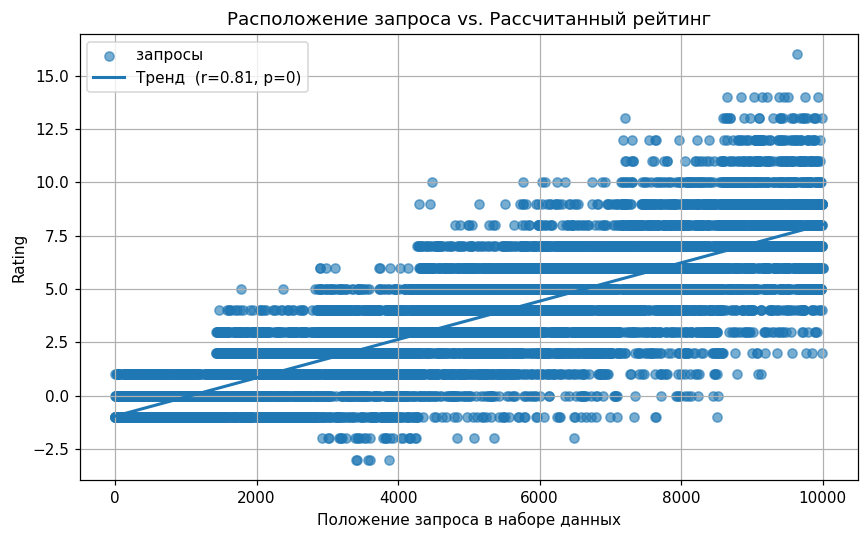
\includegraphics[width=.8\linewidth]{picture/rating-service-analitics.png}
  \caption{Диаграмма рассеяния «позиция в наборе данных»~vs.~«рейтинг» с аппроксимирующей прямой.}
\label{fig:scatter_rating}
\end{figure}

\paragraph{Интерпретация.}
Наблюдаемая тенденция подтверждает внутреннюю согласованность алгоритма: более «качественные» (по критериям \textit{PromptRatingHandler}) формулировки получают статистически значимо более высокий рейтинг. Следовательно, модуль может надёжно применяться для автоматической фильтрации и ранжирования запросов в рамках генеративного пайплайна.

\paragraph{Заключение.}
Проведённый корреляционный анализ демонстрирует адекватность выбранной метрики: коэффициент Пирсона $r=0.62$ указывает на существенную долю объяснённой дисперсии ($R^2\approx0.38$) и тем самым обосновывает использование рейтинга как доверительного индикатора качества запроса\cite{wiki:mrr}.


\subsection{Вывод}

В результате проведённой разработки создана прототипная платформа, позволяющая пользователям в интерактивном режиме формировать запросы к языковым и генеративным нейросетям и получать от них результаты. Платформа имеет современную многоуровневую архитектуру: удобный веб-интерфейс на Vue 3 обеспечивает гибкое управление запросом с помощью drag-and-drop механики, а высокопроизводительный backend на FastAPI обрабатывает запросы, обращается к внешним API генерации текста (DeepSeek) и изображений (Stable Diffusion) и обогащает ответы с помощью базы знаний (PostgreSQL/pgvector).

Поставленные задачи были успешно решены: реализован наглядный интерфейс, скрывающий сложность взаимодействия с моделями ИИ; обеспечена генерация осмысленных текстов и реалистичных изображений по запросу пользователя; продемонстрировано преимущество комбинирования разных технологий (LLM и диффузионные модели) в одном приложении. Интеграция семантического поиска позволила сделать ответы более контекстно релевантными, что повышает ценность системы для конечного пользователя.

Перспективы развития платформы включают в себя дальнейшее улучшение качества генерируемого контента и удобства взаимодействия. Во-первых, планируется расширить набор моделей: подключить более новые или специализированные языковые модели, а также модели для генерации не только статичных изображений, но и других типов медиа (например, генерация аудио или видео, если это будет доступно через API). Во-вторых, можно реализовать более сложный редактор запросов с поддержкой условной логики и циклов (чтобы пользователь мог строить цепочки вызовов моделей, задавать последовательность: например, "сгенерируй текст, потом на основе этого текста сгенерируй изображение"). В-третьих, стоит рассмотреть возможность локального развёртывания моделей с использованием GPU-серверов, чтобы снизить зависимость от внешних API и обеспечить конфиденциальность данных (особенно актуально для корпоративных пользователей). В-четвёртых, развитие системы может идти в направлении персонализации: хранение профилей пользователей, адаптация моделей под стиль пользователя на основе собранной обратной связи, создание системы подсказок и обучения пользователя эффективным стратегиям запроса.

Таким образом, разработанная платформа представляет собой основу для будущих исследований и проектов, объединяющих разнородные генеративные технологии в едином приложении. Она демонстрирует, что современные инструменты веб-разработки и машинного обучения могут быть успешно интегрированы для создания новых способов взаимодействия человека с искусственным интеллектом. Платформа может быть расширена и доработана для различных прикладных задач -- от образовательных чат-ботов до творческих студий, где пользователи сочетают генерацию текстов и изображений для реализации своих идей. Это свидетельствует о большом потенциале подобных систем и актуальности направления интерактивных средств работы с генеративными нейросетями.

\section{Экономическое обоснование разработки платформы для интерактивного формирования запросов к языковым и генеративным нейросетям}
\label{sec:economics}

\subsection{Характеристика разработанного по индивидуальному заказу  программного средства}
Разрабатываемое программное средство представляет собой интеллектуальную платформу, предназначенную для интерактивного формирования запросов (промптов) к большим языковым и генеративным нейросетям. Иными словами, это инструмент для “prompt engineering”, помогающий пользователям правильно формулировать запросы к AI-моделям с целью получения релевантных и точных результатов.
Актуальность такого решения обусловлена бурным ростом применения генеративного ИИ в бизнесе: по данным опроса McKinsey, уже через год после появления массовых генеративных моделей треть компаний регулярно использует их как минимум в одной функции бизнеса​.
Руководители компаний все чаще лично работают с инструментами GPT-подобного ИИ​.
Однако эффективность этих моделей сильно зависит от качества запроса, поэтому умение правильно задавать вопрос нейросети стало критически важным навыком​.
Разрабатываемая платформа призвана упростить этот процесс для конечных пользователей.
Основные функции, которые выполняет программное средство:
\begin{enumerate}[label=\arabic*.]
	\item Разбивать запрос на логические блоки.
	\item Генерировать предпоказ результата использования запроса.
	\item Улучшать запрос.
	\item Расширять запрос.
	\item Загружать историю запросов.
	\item Перемещать слова в запросе как drag and drop элементы.
\end{enumerate}
Экономическая оценка целесообразности инвестиций в разработку и использование программного средства осуществляется на основе расчета и оценки следующих показателей: чистый дисконтированный доход, рентабельность инвестиций и срок окупаемости инвестиций

\subsection{Расчет затрат на 	 и цены программного средства по индивидуальному заказу}

Цена программного средства определена на основе полных затрат на разработку программного средства и включает в себя следующие статьи затрат:
\begin{itemize}
	\item затраты на основную заработную плату разработчиков;
	\item затраты на дополнительную заработную плату разработчиков;
	\item отчисления на социальные нужды;
	\item прочие затраты (амортизационные отчисления, расходы на электроэнергию, командировочные расходы, арендная плата за офисные помещения и оборудование, расходы на управление и реализацию и т.п.);
	\item общая сумма затрат на разработку;
	\item плановая прибыль, включаемая в цену программного средства;
	\item отпускная цена программного средства;

\end{itemize}

1. Затраты на основную заработную плату команды разработчиков.
Основная заработная плата исполнителей проекта определяется по формуле:

\begin{equation}
	\mbox{З}_{\mbox{о}}=\mbox{К}_{\mbox{пр}}\cdot \sum_{i=1}^{n}{\mbox{З}_{\mbox{ч}i}\cdot t_{i}},
\end{equation}

где	$n$ -- количество исполнителей, занятых разработкой конкретного ПО;

$\mbox{К}_{\mbox{пр}}$ -- коэффициент премий (1,5);

$\mbox{З}_{\mbox{ч}i}$ -- часовая заработная плата i-го исполнителя (руб.);

$t_{i}$ -- трудоемкость работ, выполняемых i-м исполнителем (ч).


Разработкой программного средства занимались следующие лица: бизнес–аналитик, 2 программиста, тестировщик, дизайнер, разработчик искусственного интеллекта. Часовая заработная плата каждого исполнителя определялась путем деления его месячной заработной платы (оклад) на количество рабочих часов в месяце.

Количество рабочих часов в месяце составляет 168.

Расчет основной заработной платы представлен в таблице \ref{tab1}.

\begin{table}[!h!t]
	\caption{Расчет основной заработной платы }
	\label{tab1}
	\centering

	\begin{tabular}{| >{\raggedright}m{0.02\textwidth}
		| >{\centering\arraybackslash}m{0.22\textwidth}
		| >{\centering\arraybackslash}m{0.15\textwidth}
		| >{\centering\arraybackslash}m{0.13\textwidth}
		| >{\centering\arraybackslash}m{0.2\textwidth}
		| >{\centering\arraybackslash}m{0.12\textwidth}|}

		\hline
		№                                                                                                                        & Участник команды                      & Месячный оклад, р. & Часовой оклад, р. & Трудоемкость работ, ч. & Итого, р. \\

		\hline
		1                                                                                                                        & 2                                     & 3                  & 4                 & 5                      & 6         \\

		\hline
		1                                                                                                                        & Бизнес–аналитик                       & 4000               & 23,80             & 80                     & 1904,00   \\

		\hline
		2                                                                                                                        & Программист                           & 2980               & 17,73             & 725                    & 12860,00  \\

		\hline
		3                                                                                                                        & Тестировщик                           & 1800               & 10,71             & 400                    & 4284,00   \\

		\hline
		4                                                                                                                        & Дизайнер                              & 3647               & 21,71             & 144                    & 3129,12   \\

		\hline
		5                                                                                                                        & Разработчик искусственного интеллекта & 3000               & 17,86             & 320                    & 5715,20   \\

		\hline
		\multicolumn{5}{|l|}{Итого}                                                                                              & 27892,32                                                                                                            \\

		\hline
		\multicolumn{5}{|l|}{Премия(50\%)}                                                                                       & 13946,16                                                                                                            \\
		\hline

		\multicolumn{5}{|l|}{\begin{tabular}[c]{@{}l@{}}Итого затраты на основную заработную плату\\ разработчиков\end{tabular}} & 41838,48                                                                                                            \\
		\hline
	\end{tabular}
\end{table}

2. Затраты на дополнительную заработную плату команды разработчиков включает выплаты, предусмотренные законодательством о труде (оплата трудовых отпусков, льготных часов, времени выполнения государственных обязанностей и других выплат, не связанных с основной деятельностью исполнителей), и определяется по формуле:

\begin{equation}
	\text{З}_{\text{д}} = \frac{\text{З}_{o}\cdot H_\text{д}}{100\%},

\end{equation}


где $H_\text{д}$ -- норматив дополнительной              заработной платы(20 \%);

$\text{З}_{\text{o}}$ -- затраты на основную заработную плату, (р.);




Дополнительная заработная плата составит:

$$
	\text{З}_{\text{д}} = \frac{41838,48 \cdot 20\%}{100\%} = 8367,70 \text{ р}.
$$

3. Отчисления в фонд социальной защиты и обязательного страхования (в фонд социальной защиты населения и на обязательное страхование) определяются в соответствии с действующими законодательными актами по формуле:

\begin{equation}
	\text{Р}_{\text{соц}} = \frac{(\text{З}_{o} + \text{З}_{\text{д}})\cdot H_\text{соц}}{100\%},
\end{equation}

где $H_\text{соц}$ -- норматив отчислений в фонд социальной защиты населения и на обязательное страхование (34,6 \%).

$$
	\text{Р}_{\text{соц}} = \frac{(41838,48 + 8367,70)\cdot 34,6\%}{100\%} = 17371,34 \text{ р}.
$$

4. Прочие затраты включаются в себестоимость разработки программного обеспечения в процентах от затрат на основную заработную плату команды разработчиков (табл.2.1) по формуле:

\begin{equation}
	\text{З}_{\text{пр}} = \frac{\text{З}_{o} \cdot \text{Н}_{\text{пр}}}{100},

\end{equation}

где $\text{Н}_{\text{пр}}$ -- норматив прочих затрат (40 \%).

$$
	\text{З}_{\text{пр}} = \frac{41838,48 \cdot 40\%}{100\%} = 16735,32 \text{ р}.
$$

5. Общая сумма затрат на разработку рассчитывается путем суммирования основной заработной платы,
дополнительной заработной платы, отчислений на социальные нужды, прочих затрат. Формула расчета имеет следующий вид:

$$
	\text{З}_{\text{р}} =\text{З}_{\text{о}} + \text{З}_{\text{д}} + \text{Р}_{\text{соц}} + \text{З}_{\text{пр}}
$$

$$
	\text{З}_{\text{р}} = 41838,48+8367,70+16735,32+17371,34 = 84312,84 \text{ р}.
$$

6. Плановая прибыль включает в себя два ключевых компонента: затраты на разработку и рентабельность этих затрат. Рентабельность затрат отражает желаемую прибыльность инвестиций и показывает, какой процент от затрат на разработку составит прибыль. Формула расчета имеет следующий вид:

\begin{equation}
	\text{П}_{\text{п.с}} = \frac{\text{З}_{\text{р}} \cdot \text{Р}_{\text{п.с}}}{100\%},

\end{equation}

где $\text{Р}_{\text{п.с}}$ -- рентабельность затрат на разработку программного средства (25 \%).

$$
	\text{П}_{\text{п.с}} = \frac{84312,84  \cdot 25\%}{100\%} = 21078,21 \text{ р}.
$$

7. Отпускная цена программного средства — это стоимость, по которой продукт предлагается заказчику. Она включает в себя все затраты на разработку, маркетинг и поддержку, а также предполагаемую прибыль. Отпускная цена может варьироваться в зависимости от рыночных условий, конкуренции и уникальных характеристик программного обеспечения. Формула расчета имеет следующий вид:

\begin{equation}
	\text{Ц}_{\text{п.с}} = \text{З}_{\text{р}} + \text{П}_{\text{п.с}}
\end{equation}

$$
	\text{Ц}_{\text{п.с}} = 84312,84 + 21078,21 = 105391,05 \text{ р}.

$$


Результаты расчета затрат на разработку представлены в таблице \ref{tab2}.

\begin{table}[!h!t]
	\centering
	\caption{Затраты на разработку программного обеспечения}
	\label{tab2}
	\begin{tabular}{|l|c|}
		\hline
		\multicolumn{1}{|c|}{Статья затрат}                                                                       & Сумма, руб. \\ \hline
		Основная заработная плата команды разработчиков                                                           & 41838,48    \\ \hline
		\begin{tabular}[c]{@{}l@{}}Дополнительная заработная плата команды\\ разработчиков\end{tabular}           & 8367,70     \\ \hline
		\begin{tabular}[c]{@{}l@{}}Отчисления в фонд социальной защиты и\\ обязательного страхования\end{tabular} & 17371,34    \\ \hline
		Прочие затраты                                                                                            & 16735,32    \\ \hline
		Общая сумма затрат на разработку                                                                          & 84312,84    \\ \hline
		\begin{tabular}[c]{@{}l@{}}Плановая прибыль, включаемая в цену \\программного средства\end{tabular}       &
		21078,21                                                                                                                \\ \hline
		Отпускная цена программного средства                                                                      &
		105391,05                                                                                                               \\ \hline
	\end{tabular}

\end{table}

\subsection{Расчет результата от разработки и использования программного средства по индивидуальному заказу}

Экономический эффект от разработки программного средства по индивидуальному заказу рассчитан для организации-разработчика (резидент Парка высоких технологий) и для организации-заказчика.

1. Для организации-разработчика экономическим эффектом является прирост чистой прибыли, полученной от разработки и реализации программного средства заказчику. Так как программное средство будет реализовываться организацией-разработчиком по отпускной цене, сформированной на основе затрат на разработку, то экономический эффект, полученный организацией-разработчиком, в виде прироста чистой прибыли от его разработки, определяется по формуле::

$$
	\text{$\Delta$П}_{\text{ч}} = \text{П}_{\text{п.с}} \cdot (1 - \frac{\text{Н}_{\text{п}} }{100\%}),
$$

где $\text{Н}_{\text{п}}$ -- ставка налога на прибыль,согласно действующему законодательству, (по состоянию на 01.01.2025 г. – 	20\%).;

$\text{П}_{\text{п.с}}$ -- прибыль, включаемая в цену программного средства, (р.);

$$
	\text{$\Delta$П}_{\text{ч}} = 21078,21 \cdot (1 - \frac{20\%}{100\%}) = 16862,57 \text{ р}.
$$

Исходя из расчетов, экономический эффект составляет 16862,57 \text{ р}.


Для организации-заказчика расчет экономического эффекта от применения программного обеспечения, разработанного по индивидуальному заказу сторонней организации, выполняется по следующей методике:

1. Экономия на заработной плате и начислениях на заработную плату сотрудников за счет снижения трудоемкости работ считается по формуле:


\begin{equation}
	\text{Э}_{\text{з.п}} = \text{К}_{\text{п.р}}\cdot (t^{\text{без п.с}}_{\text{р}}-t^{\text{с п.с}}_{\text{р}})\cdot \text{Т}_{\text{ч}}\cdot N_{\text{П}}\cdot  (1+\frac{\text{Н}_{\text{д}}}{100\%})\cdot (1+\frac{\text{Н}_{\text{соц}}}{100\%}),
\end{equation}

где $N_{\text{П}}$ -- плановый объем работ;

$t^{\text{без п.с}}_{\text{р}}-t^{\text{с п.с}}_{\text{р}}$ -- трудоемкость выполнения работы до и после внедрения программного продукта, нормо-час;

$\text{Т}_{\text{ч}}$ -- часовая тарифная ставка, соответствующая разряду выполняемых работ, руб./ч (15 руб./ч.);

$\text{К}_{\text{пр}}$ -- коэффициент премий, (1,5);

$\text{Н}_{\text{д}}$ -- норматив дополнительной заработной платы, (20\%);

$\text{Н}_{\text{соц}}$ -- ставка отчислений от заработной платы, включаемых в себестоимость, (34,6\%).

$$
	\text{Э}_{\text{З}} = 1,5 \cdot (8-4)\cdot 15\cdot 168 \cdot  (1+\frac{20\%}{100\%})\cdot (1+\frac{34,6\%}{100\%}) =  24421,82 \text{ р}.

$$
2. Экономия на заработной плате и начислениях на заработную плату в результате сокращения численности работников рассчитывается по формуле:

\begin{equation}
	\text{Э}_{\text{з.п}} = \sum_{i=1}^{n}{\text{$\Delta$Ч}_{\text{i}}\cdot \text{З}_{\text{i}}\cdot  (1+\frac{\text{Н}_{\text{д}}}{100\%})\cdot (1+\frac{\text{Н}_{\text{соц}}}{100\%})},

\end{equation}

где $n$ -- категории работников, высвобождаемых в результате внедрения
программного средства (1);

$\text{$\Delta$Ч}_{\text{i}}$ -- численность работников i-й категории, высвобожденных после
внедрения программного средства, (чел.);

$\text{З}_{\text{i}}$ -- годовая заработная плата высвобожденных работников i-й категории после внедрения программного средства, (р.);

$\text{Н}_{\text{д}}$ -- норматив дополнительной заработной платы, (20\%);

$\text{Н}_{\text{соц}}$ -- ставка отчислений от заработной платы, включаемых в себестоимость, (34,6\%).

\begin{align*}
	\text{Э}_{\text{З}} & = 1 \cdot 36000 \cdot \left(1 + \frac{20\%}{100\%}\right) \cdot \left(1 + \frac{34,6\%}{100\%}\right) +       \\
	                    & \quad + 1 \cdot 48000 \cdot \left(1 + \frac{20\%}{100\%}\right) \cdot \left(1 + \frac{34,6\%}{100\%}\right) + \\
	                    & \quad + 1 \cdot 21600 \cdot \left(1 + \frac{20\%}{100\%}\right) \cdot \left(1 + \frac{34,6\%}{100\%}\right) + \\
	                    & \quad + 1 \cdot 43764 \cdot \left(1 + \frac{20\%}{100\%}\right) \cdot \left(1 + \frac{34,6\%}{100\%}\right)   \\
	                    & = 58147,20 + 77529,60 + 34888,32 + 70687,61                                                                   \\
	                    & = 241252,73 \text{ р}.

\end{align*}

Прирост чистой прибыли, полученной за счёт экономии на текущих затратах предприятия, будет рассчитываться по формуле:

\begin{equation}
	\text{$\Delta$П}_{\text{ч}} = (\text{Э}_{\text{тек}} - \text{$\Delta$З}_{\text{тек}})\cdot (1-\frac{\text{Н}_{\text{п}}}{100\%}),
\end{equation}

где $\text{Э}_{\text{тек}}$ -- экономия на текущих затратах при использовании программного средства, (р.);

$\text{$\Delta$З}_{\text{тек}}$ -- прирост текущих затрат, связанных с использованием ПО,
(р.);

$\text{Н}_{\text{п}}$ -- ставка налога на прибыль, в соответствии с действующим законодательством, (20\%).


$$
	\text{$\Delta$П}_{\text{ч}} = (120560,21 - 60182,5)\cdot (1-\frac{20\%}{100\%}) = 48302,17 \text{р}.
$$

\subsection{Расчет показателей экономической эффективности разработки и использования программного средства}

Оценка экономической эффективности разработки и использования программного средства для собственных нужд зависит от результата сравнения затрат на его разработку (модернизацию, совершенствование) и полученного экономического эффекта (годового прироста чистой прибыли).

1. Для организации-разработчика программного средства оценка экономической эффективности разработки осуществляется с помощью расчета простой нормы прибыли (рентабельности инвестиций (затрат) на разработку программного средства) по формуле:

\begin{equation}
	\text{Р}_{\text{и}} = \frac{\text{$\Delta$П}_{\text{ч}}}{\text{З}_{\text{р}}} \cdot 100\%,
\end{equation}

где $\text{$\Delta$П}_{\text{ч}}$ -- прирост чистой прибыли, полученной от разработки программного средства организацией-разработчиком по индивидуальному заказу, (р.);

$\text{З}_{\text{р}}$ -- затраты на разработку программного средства организацией-разработчиком,  (р.)


\begin{equation}
	\text{Р}_{\text{и}} = \frac{21078,21}{84312,84} \cdot 100\% = 25\%
\end{equation}

2. Поскольку сумма инвестиций меньше суммы годового экономического эффекта, то экономическая целесообразность инвестиций в разработку и использование программного продукта осуществляется на основе формулы:

\begin{equation}
	\text{Р}_{\text{и}} = |\frac{\text{$\Delta$П}_{\text{ч}}}{\text{Ц}_{\text{п.с}} \cdot (1 + \frac{\text{Н}_{\text{д.с}}}{100\%})} - 1| \cdot 100\%,
\end{equation}

где $\text{Н}_{\text{д.с}}$ -- ставка налога на добавленную стоимость в соответствии с законодательством, {\%};

$\text{Ц}_{\text{п.с}}$ -- общая сумма затрат на разработку и реализацию программного средства, (р.).

$$
	\text{Ц}_{\text{п.с}} =\text{З}_{\text{о}} + \text{З}_{\text{д}} + \text{Р}_{\text{соц}} + \text{З}_{\text{пр}} + \text{Р}_{\text{р}}
$$

где $\text{Р}_{\text{р}}$ -- расходы на реализацию.

\begin{equation}
	\text{Р}_{\text{р}} = \frac{\text{З}_{\text{о}} \cdot \text{Н}_{\text{р}}}{100\%},
\end{equation}

где $\text{Н}_{\text{р}}$ -- норматив расходов на реализацию (5\%).

\begin{equation}
	\text{Р}_{\text{р}} = \frac{41838,48 \cdot 5\%}{100\%} = 2091,92 \text{ р}.
\end{equation}

Итого значение общих затрат на разработку и реализацию:

$$
	\text{Ц}_{\text{п.с}} = 41838,48+8367,70+17371,34+16735,32+2091,92 = 86404,76 \text{ р}.
$$


Тогда экономическая целесообразность инвестиций в разработку и использование программного продукта будет равна:

\begin{equation}
	\text{Р}_{\text{и}} = |\frac{16862,57 }{86404,76 \cdot (1 + \frac{25\%}{100\%})} - 1| \cdot 100\% = 84, 39 \%.
\end{equation}

Полученное значение экономической целесообразности показывает, какую чистую прибыль компания-разработчик может получить от вложений в разработку программного
обеспечения. Поскольку объём инвестиций превышает годовой прирост чистой прибыли, для организации-заказчика дополнительно рассчитываются
другие показатели экономической эффективности
Для приведения доходов и затрат к настоящему моменту времени
определяется коэффициент дисконтирования по формуле:

\begin{equation}
	\alpha_t = \frac{1}{\text{(1 + d)}^{\text{t}-\text{t}_\text{p}}}
\end{equation}
\newpage

где $d$ – требуемая норма дисконта, которая по своему смыслу соответствует устанавливаемому инвестором желаемому уровню рентабельности инвестиций, доли единицы;
$t$  – порядковый номер года, доходы и затраты которого приводятся к расчетному году;
$tp$  – расчетный год, к которому приводятся доходы и инвестиционные затраты.

Норму дисконта принимаем равным ставке рефинансирования Национального банка Республики Беларусь – 9,5\% \cite{refr}. Расчетный период составит четыре года.

\begin{equation}
	\begin{aligned}
		\alpha_1 & = \frac{1}{(1 + 0{,}095)^0} = 1{,}000      \\
		\alpha_2 & = \frac{1}{(1 + 0{,}095)^1} \approx 0{,}91 \\
		\alpha_3 & = \frac{1}{(1 + 0{,}095)^2} \approx 0{,}83 \\
		\alpha_4 & = \frac{1}{(1 + 0{,}095)^3} \approx 0{,}76
	\end{aligned}
\end{equation}

В первый год осуществляется разработка приложения, поэтому экономический эффект в этот период будет ниже ожидаемого.
Чтобы учесть это, необходимо определить продолжительность разработки. Поскольку команда работает параллельно поэтому берём за основу наибольшее количество часов у участника
проект и составляет 720 часов. Расчет эффективности инвестиций (затрат) в реализацию проектного решения представлен в таблице \ref{tab3}.
В данном случае дисконтированный эффект нарастающим итогом превысит дисконтированные инвестиции на третий год. Дисконтированный срок окупаемости рассчитывается по формуле:
\begin{equation}
	\text{T}_{\text{ок}} = \frac{\sum_{t=1}^{n}{\text{З}_t}}{\frac{1}{n} \cdot \sum_{t=1}^{n} \Delta\text{П}_{\text{чt}}},
\end{equation}

где $n$ – расчетный период, лет;

$\text{З}_t$ – затраты (инвестиции) в году t, р.;

$\Delta\text{П}_{\text{чt}}$  – прирост чистой прибыли в году t в результате реализации проекта, р.
\begin{table}[H]
	\caption{Расчёт эффективности инвестиций}
	\label{tab3}
	\centering
	\begin{tabular}{|p{6.3cm}|c|c|c|c|}
		\hline
		\multirow{2}{6.3cm}{\textbf{Показатель}}                 & \multicolumn{4}{c|}{\textbf{Годы расчётного периода}}                               \\
		\cline{2-5}
		                                                         & 1-й год                                               & 2-й год & 3-й год & 4-й год \\
		\hline
		1.\,Прирост чистой прибыли,~р.                           &
		36\,226,63                                                        &
		48\,302,17                                              &
		48\,302,17                                              &
		48\,302,17                                                                                                                                    \\
		\hline
		2.\,Дисконтированный результат,~р.                       &
		36\,226,63                                                        &
		43\,954,97                                              &
		40\,090,80                                             &
		36\,709,65                                                                                                                                    \\
		\hline
		3.\,Инвестиции в разработку,~р.                          &
		86\,404,76                                               &
		0                                                        &
		0                                                        &
		0                                                                                                                                              \\
		\hline
		4.\,Дисконтированные инвестиции,~р.                      &
		86\,404,76                                               &
		0                                                        &
		0                                                        &
		0                                                                                                                                              \\
		\hline
		5.\,Чистый дисконтированный доход по годам,~р.           &
		-50\,178,13                                              &
		-6\,223,16                                              &
		33\,867,64                                              &
		36\,709,65                                                                                                                                    \\
		\hline
		6.\,Чистый дисконтированный доход накопленным итогом,~р. &
		-50\,178,13                                              &
		-6\,223,16                                               &
		33\,867,64                                              &
		70\,577,29                                                                                                                                    \\
		\hline
		7.\,Коэффициент дисконтирования, доли ед.                &
		1,00                                                     &
		0,91                                                     &
		0,83                                                     &
		0,76                                                                                                                                           \\
		\hline
	\end{tabular}
\end{table}


Таким образом, дисконтированный срок окупаемости равен:

\begin{equation}
	\text{T}_{\text{ок}} = \frac{86\,404{,}76}{\frac{1}{4} \cdot (36\,226,63 + 48\,302,17 + 48\,302,17 + 48\,302,17)} = 1,91 \text{ года}.
\end{equation}
\begin{equation}
	\text{ИД}_{\text{PI}} = \frac{\sum_{t=1}^{n} \text{П}_{\text{чi}} \cdot \alpha_i}{\sum_{t=1}^{n} \text{З}_{i} \cdot \alpha_i}
\end{equation}

Таким образом, индекс доходности инвестиций равен:

\begin{equation}
	\text{ИД}_{\text{PI}} = \frac{36\,226,63 +43\,954,97 + 40\,090,80 + 36\,709,65}{86\,404,76} = 1,81.
\end{equation}

\newpage
\subsection{Вывод}

В результате технико-экономического обоснования разработкиа платформы для интерактивного формирования
запросов к языковым и генеративным нейросетям были получены следующие значения показателей эффективности:

\begin{enumerate}{locale=\arabic*.}
	\item Рентабельность инвестиций организации-разработчика составляет 25 \%.
	\item Затраты на разработку программного продукта окупятся.
	\item Рентабельность инвестиций организации-заказчика составляет 84,39 \%.

\end{enumerate}

Таким образом, разработка и применение программного продукта является эффективной и данные инвестиции осуществлять целесообразно.

\sectioncentered*{Заключение}
\addcontentsline{toc}{section}{Заключение}

В ходе выполнения дипломной работы изучены существующие методы интерактивного формирования запросов к языковым и генеративным нейросетям, а также исследованы современные подходы к интеграции с внешними нейросетевыми сервисами. На основании проведенного анализа сформулированы функциональные требования к разрабатываемой платформе. Также предложена её архитектура в виде клиент-серверного приложения с разделением на клиентскую и серверную части (Frontend + Backend).

В соответствии с сформулированными требованиями разработана программная платформа с архитектурой «клиент-сервер»: клиентская часть реализована на базе JavaScript-фреймворка Vue.js, серверная — на базе Python-фреймворка FastAPI. Пользовательский интерфейс системы обеспечивает визуальное конструирование запросов методом «drag-and-drop». Для хранения данных о запросах и результатах используется база данных PostgreSQL с модулем pgvector, позволяющим сохранять векторные представления данных и выполнять по ним поиск. Реализована интеграция с внешними API: FusionBrain (для генерации изображений) и DeepSeek (для обработки естественного языка). Алгоритмы обработки пользовательских запросов на стороне сервера автоматически преобразуют сформированные визуальные схемы в последовательность вызовов нейросетевых моделей.

Разработанная платформа испытана в различных сценариях использования, подтвердивших корректность её работы и соответствие предъявленным требованиям. Экспериментально показано, что предложенное решение эффективно автоматизирует процесс формирования сложных запросов к языковым и генеративным моделям, повышая удобство и эффективность использования нейросетей. Также выполнено технико-экономическое обоснование проекта. Анализ показал, что применение современных открытых инструментов (Vue, FastAPI, PostgreSQL) и внешних API (FusionBrain, DeepSeek) обеспечивает высокую функциональность системы при оптимальных затратах, подтверждая целесообразность её внедрения. Таким образом, цель дипломной работы достигнута: разработана и исследована платформа для интерактивного формирования запросов к языковым и генеративным нейросетям, продемонстрировавшая практическую применимость и эффективность предложенного подхода.

% If you want to list ALL entries from the .bib file, uncomment \nocite{*}
\nocite{*}

% Use normal (roman) font for URLs instead of typewriter
\urlstyle{rm}
\phantomsection\pagebreak% исправляет нумерацию в документе и исправляет гиперссылки в pdf

% Use your custom Belarus-specific BibTeX style
\bibliographystyle{./biblio/belarus-specific-utf8gost780u.bst}
% Specify your .bib file (no .bib extension needed)
\bibliography{./biblio/othercites.bib}


\newgeometry{left=1.5cm,top=2.0cm,right=1.5cm,bottom=2.7cm}
\pagestyle{empty}

\begin{figure}[p]
    \centering
     \hspace*{-2em}
    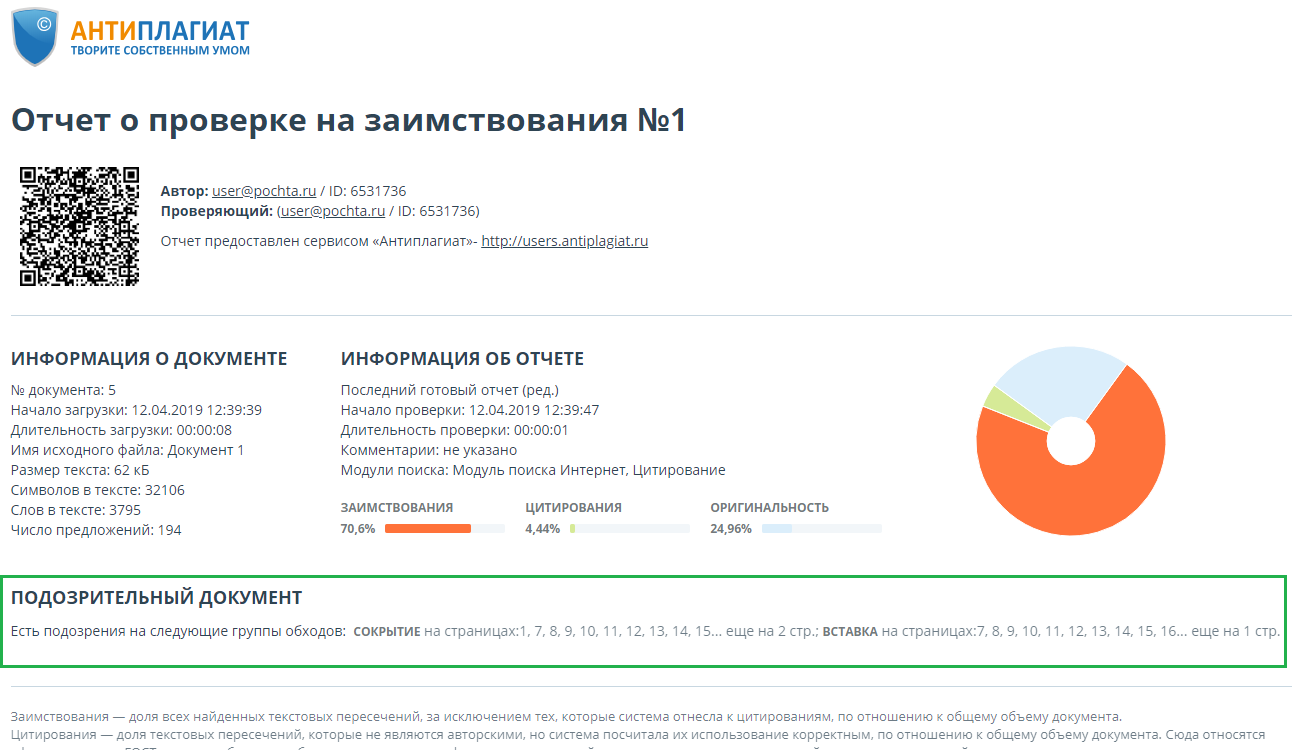
\includegraphics[width=1\linewidth, angle=90]{picture/bypass-short-report-print-private.png}
%    \caption{Enter Caption}
    \label{fig:enter-label}
\end{figure}
% Если в тексте записки есть приложения, для добавления их в содержание, необходимо оставить следующую строку
% Если приложений нет - данную строку добавляем в комментарий


% Если в тексте записки есть приложения, для добавления их в содержание, необходимо оставить следующую строку
% Если приложений нет - данную строку добавляем в комментарий
%\appendix
\intro{А}{обязательное}{Пример оформления}
%\addcontentsline{toc}{section}{Приложения}
Текст приложения.

\appendix
\intro{B}{справочное}{Пример оформления}
%\addcontentsline{toc}{section}{Приложения}
Текст приложения.

\newgeometry{left=1.5cm,top=2.0cm,right=1.5cm,bottom=2.7cm}
\thispagestyle{empty}

\hskip-2em
\begin{tabular}{|p{15pt}|p{10pt}|p{80pt}|p{20pt}|p{20pt}|p{150pt}|p{5pt}|p{5pt}|p{5pt}|p{30pt}|p{30pt}|}
\hline

\multicolumn{5}{|p{145pt}|} {\centering\textit{Обозначение}} & \multicolumn{4}{|p{200pt}|} {\centering\textit{Наименование}} & \multicolumn{2}{|p{80pt}|} {\centering\textit{Дополни- тельные сведения}}\\\hline

\multicolumn{5}{|p{145pt}|} {} & \multicolumn{4}{|p{200pt}|} {\underline{Текстовые документы}} & \multicolumn{2}{|p{80pt}|} {} \\\hline

\multicolumn{5}{|p{145pt}|} {} & \multicolumn{4}{|p{200pt}|} {} & \multicolumn{2}{|p{80pt}|} {} \\\hline
%БГУИР ДП 1-40 03 01 02 XХX ПЗ - шифр как на титульном листе
\multicolumn{5}{|p{145pt}|} {БГУИР ДП 1-40 03 01 054 ПЗ} & \multicolumn{4}{|p{200pt}|} {Пояснительная записка} & \multicolumn{2}{|p{80pt}|} {\centering \pageref*{LastPage}~c.} \\\hline

\multicolumn{5}{|p{145pt}|} {} & \multicolumn{4}{|p{200pt}|} {Отзыв руководителя} & \multicolumn{2}{|p{80pt}|} {} \\\hline

\multicolumn{5}{|p{145pt}|} {} & \multicolumn{4}{|p{200pt}|} {Рецензия} & \multicolumn{2}{|p{80pt}|} {} \\\hline

\multicolumn{5}{|p{145pt}|} {} & \multicolumn{4}{|p{200pt}|} {Справка о внедрении результа-} & \multicolumn{2}{|p{80pt}|} {} \\\hline
\multicolumn{5}{|p{145pt}|} {} & \multicolumn{4}{|p{200pt}|} {тов} & \multicolumn{2}{|p{80pt}|} {} \\\hline

%\multicolumn{5}{|p{145pt}|} {} & \multicolumn{4}{|p{200pt}|} {Акт внедерения результатов в учебный процесс} & \multicolumn{2}{|p{80pt}|} {} \\\hline

\multicolumn{5}{|p{145pt}|} {} & \multicolumn{4}{|p{200pt}|} {Отчет о проверке дипломного} & \multicolumn{2}{|p{80pt}|} {} \\\hline

\multicolumn{5}{|p{145pt}|} {} & \multicolumn{4}{|p{200pt}|} {проекта на заимствования} & \multicolumn{2}{|p{80pt}|} {} \\\hline

\multicolumn{5}{|p{145pt}|} {} & \multicolumn{4}{|p{200pt}|} {\underline{Графический материал}} & \multicolumn{2}{|p{80pt}|} {} \\\hline

\multicolumn{5}{|p{145pt}|} {} & \multicolumn{4}{|p{200pt}|} {} & \multicolumn{2}{|p{80pt}|} {} \\\hline

\multicolumn{5}{|p{145pt}|} {ГУИР.121703.001 ПЛ} & \multicolumn{4}{|p{200pt}|} {Диаграмма вариантов использо} & \multicolumn{2}{|p{80pt}|} {Формат А1} \\\hline
\multicolumn{5}{|p{145pt}|} {} & \multicolumn{4}{|p{200pt}|} {вания платформы} & \multicolumn{2}{|p{80pt}|} {} \\\hline

\multicolumn{5}{|p{145pt}|} {ГУИР.121703.002 ПЛ} & \multicolumn{4}{|p{200pt}|} {Алгоритм оценки качества за-} & \multicolumn{2}{|p{80pt}|} {Формат А1} \\\hline
\multicolumn{5}{|p{145pt}|} {} & \multicolumn{4}{|p{200pt}|} {проса} & \multicolumn{2}{|p{80pt}|} {} \\\hline

\multicolumn{5}{|p{145pt}|} {ГУИР.121703.003 ПЛ} & \multicolumn{4}{|p{200pt}|} {Интерфейс платформы} & \multicolumn{2}{|p{80pt}|} {Формат А1} \\\hline

\multicolumn{5}{|p{145pt}|} {ГУИР.121703.004 ПЛ} & \multicolumn{4}{|p{200pt}|} {Диаграмма базы данных} & \multicolumn{2}{|p{80pt}|} {Формат А1} \\\hline

\multicolumn{5}{|p{145pt}|} {ГУИР.121703.005 ПЛ} & \multicolumn{4}{|p{200pt}|} {Диаграмма структуры запроса} & \multicolumn{2}{|p{80pt}|} {Формат А1} \\\hline

\multicolumn{5}{|p{145pt}|} {ГУИР.121703.006 ПЛ} & \multicolumn{4}{|p{200pt}|} {Диаграмма структуры плат-} & \multicolumn{2}{|p{80pt}|} {Формат А1} \\\hline
\multicolumn{5}{|p{145pt}|} {} & \multicolumn{4}{|p{200pt}|} {формы} & \multicolumn{2}{|p{80pt}|} {} \\\hline

\multicolumn{5}{|p{145pt}|} {} & \multicolumn{4}{|p{200pt}|} {Электронный носитель инфор-} & \multicolumn{2}{|p{80pt}|} {CD-R} \\\hline

\multicolumn{5}{|p{145pt}|} {} & \multicolumn{4}{|p{200pt}|} {мации с программным обеспече-} & \multicolumn{2}{|p{80pt}|} {} \\\hline

\multicolumn{5}{|p{145pt}|} {} & \multicolumn{4}{|p{200pt}|} {нием и материалами.} & \multicolumn{2}{|p{80pt}|} {} \\\hline


% XXX - номер в соответствии с приказом
& & & & & \multicolumn{6}{|c|} { \multirow{3} {280pt}{\centering\textit{БГУИР ДП 1-~40 03 01 054  Д1}}} \tabularnewline \cline{1-5}
& & & & & \multicolumn{6}{|c|}{}\\\cline{1-5}
& & & & & \multicolumn{6}{|c|}{}\\\hline
% 
\centering\textit{\scriptsizeИзм.}&\centering\textit{\scriptsizeЛ.} &\centering\textit{\scriptsize№ докум.} &\centering\textit{\scriptsizeПодп.} &\centering\textit{\scriptsizeДата} & \multirow{6}{150pt}{\centering\textit{\small{Платформа для интерактивного формирования
запросов к языковым и генеративным нейросетям}}\\ \textit{\scriptsizeВедомость документов}} & \multicolumn{3}{|p{15pt}|}{\centering\textit{\footnotesizeЛит}} & \centering\textit{\footnotesizeЛист} & \centering\textit{\footnotesizeЛистов} \tabularnewline\cline{1-5} \cline{7-11}

\multicolumn{2}{|p{35pt}|}{\textit{\footnotesizeРазраб.}} & \textit{\footnotesizeСамохвал} & & & & & \textit{\footnotesize T} & & \centering\textit{\footnotesize \pageref*{LastPage}} & \centering\textit{\footnotesize \pageref*{LastPage}} \tabularnewline\cline{1-5} \cline{7-11}

\multicolumn{2}{|p{35pt}|}{\textit{\footnotesizeПров.}} & \textit{\footnotesizeКрапивин} & & & & \multicolumn{5}{|c|}{} \\\cline{1-5}

\multicolumn{2}{|p{35pt}|}{\textit{\footnotesizeТ.контр.}} & \textit{\footnotesizeКрапивин} & & & & \multicolumn{5}{|c|}{\textit{Кафедра ИИТ}} \\\cline{1-5}

% xxxxxx - номер группы
\multicolumn{2}{|p{35pt}|}{\textit{\footnotesizeН.контр.}} &\textit{\footnotesize Самодумкин} &\textit{\footnotesize} &\textit{\footnotesize} & & \multicolumn{5}{|c|}{\textit{гр. 121703}} \\\cline{1-5}

\multicolumn{2}{|p{35pt}|}{\textit{\footnotesizeУтв.}} &\textit{\footnotesize Шункевич} & & & & \multicolumn{5}{|c|}{} \\\hline

\end{tabular}
\restoregeometry

%\includepdf позволяет включить в результирующий pdf документ часть другого pdf документа
%\includepdf[pages={-}]{documents_list.pdf}

\end{document}
